\documentclass[aspectratio=1610,xcolor=svgnames]{beamer}

\usetheme{metropolis}


\usepackage{appendixnumberbeamer}
\usepackage{tikz}
\usepackage[absolute,overlay]{textpos}
\usepackage{pstricks}
%\usepackage[texcoord,grid,gridunit=mm,gridcolor=red!10,subgridcolor=green!10]{eso-pic}

\newcommand{\tikzdbg}{%
  \draw[step=1,color=lightgray] (-7,0) grid (7,7);%
  \fill[red] (0,0) circle (0.2);%
}

\title{Deadline scheduling in the Linux kernel}
\subtitle{Juri Lelli, Claudio Scordino, Luca Abeni and Dario Faggioli}
\date{July 8, 2019}
\author{Benno Fünfstück}

\begin{document}

\tikzset{
  onslide/.code args={<#1>#2}{%
    \only<#1>{\pgfkeysalso{#2}}% \pgfkeysalso doesn't change the path
  },
  temporal/.code args={<#1>#2#3#4}{%
    \temporal<#1>{\pgfkeysalso{#2}}{\pgfkeysalso{#3}}{\pgfkeysalso{#4}}%
  },
  hidden/.style = {opacity=0},
  uncover/.style = {temporal=#1{hidden}{}{}},
}

\maketitle

\section{Introduction}

\begin{frame}\frametitle{Story: A new coffee machine}
  \vspace{1cm}
  \begin{columns}
    \begin{column}{0.5\textwidth}
      
\includegraphics[width=0.95\textwidth]{coffee.pdf}
    \end{column}
    \begin{column}{0.5\textwidth}
      {\Large Components:}
      \begin{itemize}
      \item Brewing controller
      \item User interface controller
      \item Web interface
      \end{itemize}
      \vspace{1cm}
    \end{column}
  \end{columns}
\end{frame}

\begin{frame}\frametitle{Linux for real-time}
  First approach: run Linux as a task in real-time hypervisor
  \begin{itemize}
  \item examples: RTAI, RTLinux, Xenomai
  \item maintenance of HAL and microkernel for real-time
  \item custom tools and API necessary for real-time part 
  \end{itemize}

  \pause

  Second approach: make the Linux kernel itself suitable for real-time
  \begin{itemize}
  \item PREEMPT\_RT patchset
  \item<3-> \alert{real-time scheduler}
  \end{itemize}
\end{frame}

\section{Design of a realtime scheduler}

\begin{frame}\frametitle{Scheduler requirements}
  \textit{Predictability:} worst-case behaviour must be apparent
  \begin{itemize}
    \item 
  \end{itemize}

  \textit{Temporal isolation:} other tasks should not negatively affect our task
\end{frame}

\begin{frame}\frametitle{Two important properties}
  \begin{itemize}
    \item Predictability
    \item Temporal isolation
  \end{itemize}
\end{frame}

\begin{frame}
  \frametitle{Todo}
  
  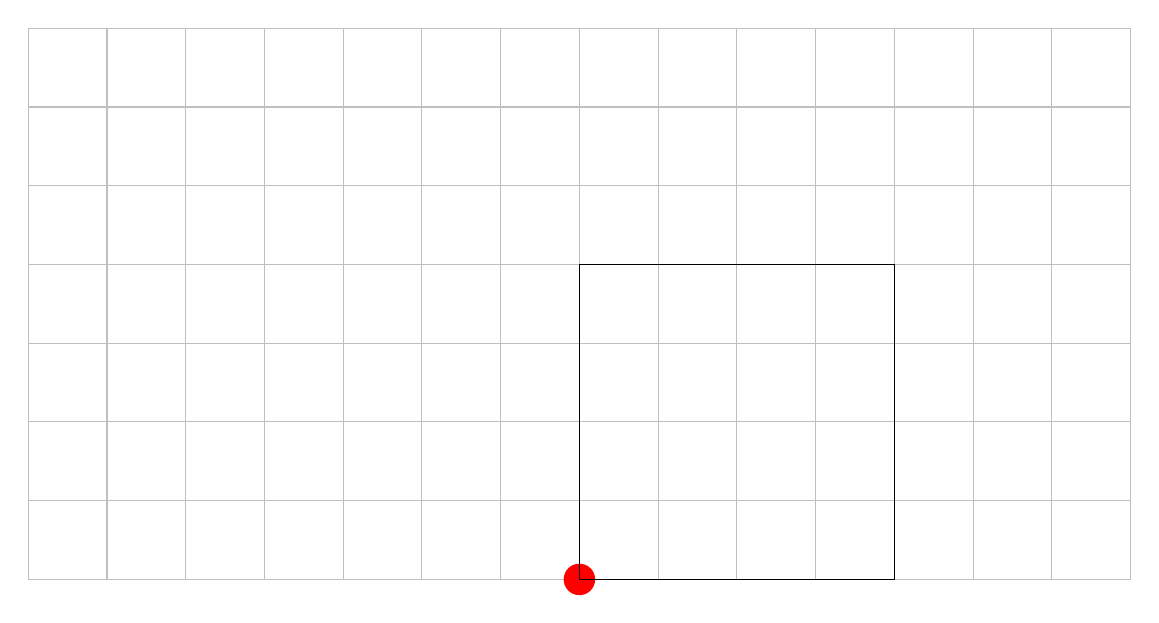
\begin{tikzpicture}
    \tikzdbg
    \draw (0,0) -- (4,0) -- (4,4) -- (0,4) -- (0,0);
  \end{tikzpicture}
\end{frame}

\section{Evaluation}

\begin{frame}\frametitle{Synthetic workload}
\end{frame}

\begin{frame}\frametitle{MPlayer on loaded system}
  \begin{center}
    %LaTeX with PSTricks extensions
%%Creator: inkscape 0.92.4
%%Please note this file requires PSTricks extensions
\psset{xunit=0.95pt,yunit=0.95pt,runit=0.95pt}
\begin{pspicture}(321.15466309,224.16531372)
{
\newrgbcolor{curcolor}{0.13725491 0.12156863 0.1254902}
\pscustom[linewidth=0.44666667,linecolor=curcolor]
{
\newpath
\moveto(28.37600244,23.46533088)
\lineto(31.19066904,23.46533088)
}
}
{
\newrgbcolor{curcolor}{0.13725491 0.12156863 0.1254902}
\pscustom[linewidth=0.44666667,linecolor=curcolor]
{
\newpath
\moveto(308.10799545,23.46533088)
\lineto(305.29199552,23.46533088)
}
}
{
\newrgbcolor{curcolor}{0.13725491 0.12156863 0.1254902}
\pscustom[linestyle=none,fillstyle=solid,fillcolor=curcolor]
{
\newpath
\moveto(22.42800259,25.93066415)
\curveto(21.61866928,25.93066415)(21.24933596,25.08266417)(21.24933596,23.67466421)
\curveto(21.24933596,22.26799758)(21.61866928,21.4199976)(22.42800259,21.4199976)
\curveto(23.23733591,21.4199976)(23.60666923,22.26799758)(23.60666923,23.67466421)
\curveto(23.60666923,25.08266417)(23.23733591,25.93066415)(22.42800259,25.93066415)
\closepath
\moveto(22.42800259,20.78799762)
\curveto(20.80933597,20.78799762)(20.49600264,22.50799757)(20.49600264,23.67466421)
\curveto(20.49600264,24.84266418)(20.80933597,26.5613308)(22.42800259,26.5613308)
\curveto(24.04666922,26.5613308)(24.36000254,24.84266418)(24.36000254,23.67466421)
\curveto(24.36000254,22.50799757)(24.04666922,20.78799762)(22.42800259,20.78799762)
}
}
{
\newrgbcolor{curcolor}{0.13725491 0.12156863 0.1254902}
\pscustom[linewidth=0.44666667,linecolor=curcolor]
{
\newpath
\moveto(28.37600244,43.21333039)
\lineto(31.19066904,43.21333039)
}
}
{
\newrgbcolor{curcolor}{0.13725491 0.12156863 0.1254902}
\pscustom[linewidth=0.44666667,linecolor=curcolor]
{
\newpath
\moveto(308.10799545,43.21333039)
\lineto(305.29199552,43.21333039)
}
}
{
\newrgbcolor{curcolor}{0.13725491 0.12156863 0.1254902}
\pscustom[linestyle=none,fillstyle=solid,fillcolor=curcolor]
{
\newpath
\moveto(15.74666943,45.69066366)
\curveto(14.93733611,45.69066366)(14.56800279,44.84266368)(14.56800279,43.43599705)
\curveto(14.56800279,42.02799708)(14.93733611,41.17999711)(15.74666943,41.17999711)
\curveto(16.55600274,41.17999711)(16.92533606,42.02799708)(16.92533606,43.43599705)
\curveto(16.92533606,44.84266368)(16.55600274,45.69066366)(15.74666943,45.69066366)
\closepath
\moveto(15.74666943,40.54933045)
\curveto(14.1280028,40.54933045)(13.81466947,42.26933041)(13.81466947,43.43599705)
\curveto(13.81466947,44.60399702)(14.1280028,46.32266364)(15.74666943,46.32266364)
\curveto(17.36533605,46.32266364)(17.67866938,44.60399702)(17.67866938,43.43599705)
\curveto(17.67866938,42.26933041)(17.36533605,40.54933045)(15.74666943,40.54933045)
}
}
{
\newrgbcolor{curcolor}{0.13725491 0.12156863 0.1254902}
\pscustom[linestyle=none,fillstyle=solid,fillcolor=curcolor]
{
\newpath
\moveto(18.67066935,40.70131712)
\lineto(19.504536,40.70131712)
\lineto(19.504536,41.54930376)
\lineto(18.67066935,41.54930376)
\closepath
}
}
{
\newrgbcolor{curcolor}{0.13725491 0.12156863 0.1254902}
\pscustom[linestyle=none,fillstyle=solid,fillcolor=curcolor]
{
\newpath
\moveto(23.07733591,40.70133045)
\lineto(22.32400259,40.70133045)
\lineto(22.32400259,44.69066368)
\lineto(21.00933596,44.69066368)
\lineto(21.00933596,45.25066367)
\curveto(21.92266927,45.31466367)(22.3000026,45.40266367)(22.52400259,46.32266364)
\lineto(23.07733591,46.32266364)
\lineto(23.07733591,40.70133045)
}
}
{
\newrgbcolor{curcolor}{0.13725491 0.12156863 0.1254902}
\pscustom[linewidth=0.44666667,linecolor=curcolor]
{
\newpath
\moveto(28.37600244,63.00532989)
\lineto(31.19066904,63.00532989)
}
}
{
\newrgbcolor{curcolor}{0.13725491 0.12156863 0.1254902}
\pscustom[linewidth=0.44666667,linecolor=curcolor]
{
\newpath
\moveto(308.10799545,63.00532989)
\lineto(305.29199552,63.00532989)
}
}
{
\newrgbcolor{curcolor}{0.13725491 0.12156863 0.1254902}
\pscustom[linestyle=none,fillstyle=solid,fillcolor=curcolor]
{
\newpath
\moveto(15.74666943,65.45066317)
\curveto(14.93733611,65.45066317)(14.56800279,64.60399652)(14.56800279,63.19599656)
\curveto(14.56800279,61.78799659)(14.93733611,60.94132995)(15.74666943,60.94132995)
\curveto(16.55600274,60.94132995)(16.92533606,61.78799659)(16.92533606,63.19599656)
\curveto(16.92533606,64.60399652)(16.55600274,65.45066317)(15.74666943,65.45066317)
\closepath
\moveto(15.74666943,60.30932996)
\curveto(14.1280028,60.30932996)(13.81466947,62.02932992)(13.81466947,63.19599656)
\curveto(13.81466947,64.36399653)(14.1280028,66.08266315)(15.74666943,66.08266315)
\curveto(17.36533605,66.08266315)(17.67866938,64.36399653)(17.67866938,63.19599656)
\curveto(17.67866938,62.02932992)(17.36533605,60.30932996)(15.74666943,60.30932996)
}
}
{
\newrgbcolor{curcolor}{0.13725491 0.12156863 0.1254902}
\pscustom[linestyle=none,fillstyle=solid,fillcolor=curcolor]
{
\newpath
\moveto(18.67066935,60.46131662)
\lineto(19.504536,60.46131662)
\lineto(19.504536,61.30938327)
\lineto(18.67066935,61.30938327)
\closepath
}
}
{
\newrgbcolor{curcolor}{0.13725491 0.12156863 0.1254902}
\pscustom[linestyle=none,fillstyle=solid,fillcolor=curcolor]
{
\newpath
\moveto(20.55333597,64.0666632)
\curveto(20.55333597,65.89866315)(21.89200261,66.08266315)(22.50133592,66.08266315)
\curveto(23.47866923,66.08266315)(24.26400255,65.45066317)(24.26400255,64.40266319)
\curveto(24.26400255,63.39599655)(23.59866923,62.97199656)(22.75733592,62.52399657)
\lineto(22.1720026,62.20532991)
\curveto(21.40266928,61.77999659)(21.23466929,61.3399966)(21.20266929,61.12532994)
\lineto(24.26400255,61.12532994)
\lineto(24.26400255,60.46132996)
\lineto(20.40933598,60.46132996)
\curveto(20.44933598,61.62932993)(20.97733596,62.25332991)(21.73200261,62.69199657)
\lineto(22.47733592,63.12399656)
\curveto(23.07866924,63.46799655)(23.51066923,63.69999654)(23.51066923,64.43599652)
\curveto(23.51066923,64.88399651)(23.22266924,65.45066317)(22.39733593,65.45066317)
\curveto(21.33066929,65.45066317)(21.28266929,64.45866319)(21.25866929,64.0666632)
\lineto(20.55333597,64.0666632)
}
}
{
\newrgbcolor{curcolor}{0.13725491 0.12156863 0.1254902}
\pscustom[linewidth=0.44666667,linecolor=curcolor]
{
\newpath
\moveto(28.37600244,82.7533294)
\lineto(31.19066904,82.7533294)
}
}
{
\newrgbcolor{curcolor}{0.13725491 0.12156863 0.1254902}
\pscustom[linewidth=0.44666667,linecolor=curcolor]
{
\newpath
\moveto(308.10799545,82.7533294)
\lineto(305.29199552,82.7533294)
}
}
{
\newrgbcolor{curcolor}{0.13725491 0.12156863 0.1254902}
\pscustom[linestyle=none,fillstyle=solid,fillcolor=curcolor]
{
\newpath
\moveto(15.74666943,85.21198267)
\curveto(14.93733611,85.21198267)(14.56800279,84.36398269)(14.56800279,82.95598273)
\curveto(14.56800279,81.5493161)(14.93733611,80.70131612)(15.74666943,80.70131612)
\curveto(16.55600274,80.70131612)(16.92533606,81.5493161)(16.92533606,82.95598273)
\curveto(16.92533606,84.36398269)(16.55600274,85.21198267)(15.74666943,85.21198267)
\closepath
\moveto(15.74666943,80.06931613)
\curveto(14.1280028,80.06931613)(13.81466947,81.78931609)(13.81466947,82.95598273)
\curveto(13.81466947,84.1239827)(14.1280028,85.84264932)(15.74666943,85.84264932)
\curveto(17.36533605,85.84264932)(17.67866938,84.1239827)(17.67866938,82.95598273)
\curveto(17.67866938,81.78931609)(17.36533605,80.06931613)(15.74666943,80.06931613)
}
}
{
\newrgbcolor{curcolor}{0.13725491 0.12156863 0.1254902}
\pscustom[linestyle=none,fillstyle=solid,fillcolor=curcolor]
{
\newpath
\moveto(18.67066935,80.22131613)
\lineto(19.504536,80.22131613)
\lineto(19.504536,81.06938278)
\lineto(18.67066935,81.06938278)
\closepath
}
}
{
\newrgbcolor{curcolor}{0.13725491 0.12156863 0.1254902}
\pscustom[linestyle=none,fillstyle=solid,fillcolor=curcolor]
{
\newpath
\moveto(21.9960026,83.41998272)
\curveto(22.1160026,83.41198272)(22.24533593,83.40398272)(22.36400259,83.40398272)
\curveto(22.91066925,83.40398272)(23.43866923,83.61998271)(23.43866923,84.32398269)
\curveto(23.43866923,84.65998269)(23.23866924,85.21198267)(22.39733593,85.21198267)
\curveto(21.39466928,85.21198267)(21.33066929,84.39464936)(21.29866929,84.0039827)
\lineto(20.60933597,84.0039827)
\curveto(20.60933597,84.82798268)(20.94533596,85.84264932)(22.42933593,85.84264932)
\curveto(23.51866923,85.84264932)(24.16800255,85.21998267)(24.16800255,84.36398269)
\curveto(24.16800255,83.64398271)(23.75066923,83.29998272)(23.44666923,83.20398272)
\lineto(23.44666923,83.18798272)
\curveto(23.99200255,83.01198273)(24.38533588,82.62798274)(24.38533588,81.87731609)
\curveto(24.38533588,80.95731611)(23.79200256,80.06931613)(22.35600259,80.06931613)
\curveto(21.9400026,80.06931613)(21.58666928,80.17331613)(21.31466929,80.31864946)
\curveto(20.68933597,80.64531612)(20.52133597,81.2933161)(20.47333597,81.94131609)
\lineto(21.20266929,81.94131609)
\curveto(21.22666929,81.4133161)(21.35466929,80.70131612)(22.40533593,80.70131612)
\curveto(23.12666924,80.70131612)(23.63200256,81.14131611)(23.63200256,81.78931609)
\curveto(23.63200256,82.73198273)(22.79733592,82.82131606)(22.3160026,82.82131606)
\curveto(22.2120026,82.82131606)(22.1000026,82.81331607)(21.9960026,82.81331607)
\lineto(21.9960026,83.41998272)
}
}
{
\newrgbcolor{curcolor}{0.13725491 0.12156863 0.1254902}
\pscustom[linewidth=0.44666667,linecolor=curcolor]
{
\newpath
\moveto(28.37600244,102.50132891)
\lineto(31.19066904,102.50132891)
}
}
{
\newrgbcolor{curcolor}{0.13725491 0.12156863 0.1254902}
\pscustom[linewidth=0.44666667,linecolor=curcolor]
{
\newpath
\moveto(308.10799545,102.50132891)
\lineto(305.29199552,102.50132891)
}
}
{
\newrgbcolor{curcolor}{0.13725491 0.12156863 0.1254902}
\pscustom[linestyle=none,fillstyle=solid,fillcolor=curcolor]
{
\newpath
\moveto(15.74666943,104.97198218)
\curveto(14.93733611,104.97198218)(14.56800279,104.1239822)(14.56800279,102.71731557)
\curveto(14.56800279,101.3093156)(14.93733611,100.46131562)(15.74666943,100.46131562)
\curveto(16.55600274,100.46131562)(16.92533606,101.3093156)(16.92533606,102.71731557)
\curveto(16.92533606,104.1239822)(16.55600274,104.97198218)(15.74666943,104.97198218)
\closepath
\moveto(15.74666943,99.83064897)
\curveto(14.1280028,99.83064897)(13.81466947,101.55064893)(13.81466947,102.71731557)
\curveto(13.81466947,103.88531554)(14.1280028,105.60398216)(15.74666943,105.60398216)
\curveto(17.36533605,105.60398216)(17.67866938,103.88531554)(17.67866938,102.71731557)
\curveto(17.67866938,101.55064893)(17.36533605,99.83064897)(15.74666943,99.83064897)
}
}
{
\newrgbcolor{curcolor}{0.13725491 0.12156863 0.1254902}
\pscustom[linestyle=none,fillstyle=solid,fillcolor=curcolor]
{
\newpath
\moveto(18.67066935,99.9826623)
\lineto(19.504536,99.9826623)
\lineto(19.504536,100.83030228)
\lineto(18.67066935,100.83030228)
\closepath
}
}
{
\newrgbcolor{curcolor}{0.13725491 0.12156863 0.1254902}
\pscustom[linestyle=none,fillstyle=solid,fillcolor=curcolor]
{
\newpath
\moveto(21.04933596,101.95732892)
\lineto(22.86133591,101.95732892)
\lineto(22.86133591,104.50799552)
\lineto(22.84533592,104.50799552)
\closepath
\moveto(23.56666923,101.34932893)
\lineto(23.56666923,99.9826623)
\lineto(22.86133591,99.9826623)
\lineto(22.86133591,101.34932893)
\lineto(20.40000264,101.34932893)
\lineto(20.40000264,102.03732892)
\lineto(22.98133591,105.60266216)
\lineto(23.56666923,105.60266216)
\lineto(23.56666923,101.95732892)
\lineto(24.39200254,101.95732892)
\lineto(24.39200254,101.34932893)
\lineto(23.56666923,101.34932893)
}
}
{
\newrgbcolor{curcolor}{0.13725491 0.12156863 0.1254902}
\pscustom[linewidth=0.44666667,linecolor=curcolor]
{
\newpath
\moveto(28.37600244,122.29466174)
\lineto(31.19066904,122.29466174)
}
}
{
\newrgbcolor{curcolor}{0.13725491 0.12156863 0.1254902}
\pscustom[linewidth=0.44666667,linecolor=curcolor]
{
\newpath
\moveto(308.10799545,122.29466174)
\lineto(305.29199552,122.29466174)
}
}
{
\newrgbcolor{curcolor}{0.13725491 0.12156863 0.1254902}
\pscustom[linestyle=none,fillstyle=solid,fillcolor=curcolor]
{
\newpath
\moveto(15.74666943,124.73198168)
\curveto(14.93733611,124.73198168)(14.56800279,123.8839817)(14.56800279,122.47731507)
\curveto(14.56800279,121.06931511)(14.93733611,120.22131513)(15.74666943,120.22131513)
\curveto(16.55600274,120.22131513)(16.92533606,121.06931511)(16.92533606,122.47731507)
\curveto(16.92533606,123.8839817)(16.55600274,124.73198168)(15.74666943,124.73198168)
\closepath
\moveto(15.74666943,119.59064848)
\curveto(14.1280028,119.59064848)(13.81466947,121.31064844)(13.81466947,122.47731507)
\curveto(13.81466947,123.64531504)(14.1280028,125.36398167)(15.74666943,125.36398167)
\curveto(17.36533605,125.36398167)(17.67866938,123.64531504)(17.67866938,122.47731507)
\curveto(17.67866938,121.31064844)(17.36533605,119.59064848)(15.74666943,119.59064848)
}
}
{
\newrgbcolor{curcolor}{0.13725491 0.12156863 0.1254902}
\pscustom[linestyle=none,fillstyle=solid,fillcolor=curcolor]
{
\newpath
\moveto(18.67066935,119.74266181)
\lineto(19.504536,119.74266181)
\lineto(19.504536,120.59039512)
\lineto(18.67066935,120.59039512)
\closepath
}
}
{
\newrgbcolor{curcolor}{0.13725491 0.12156863 0.1254902}
\pscustom[linestyle=none,fillstyle=solid,fillcolor=curcolor]
{
\newpath
\moveto(21.37866929,123.01332839)
\curveto(21.61866928,123.19732839)(21.9640026,123.36532838)(22.46800259,123.36532838)
\curveto(23.38266924,123.36532838)(24.32133588,122.72399507)(24.32133588,121.56532843)
\curveto(24.32133588,120.94132845)(24.04000255,119.59066181)(22.2760026,119.59066181)
\curveto(21.53866928,119.59066181)(20.59333597,119.8866618)(20.45733597,121.14266177)
\lineto(21.18533596,121.14266177)
\curveto(21.25866929,120.48532846)(21.74666928,120.1986618)(22.38133593,120.1986618)
\curveto(23.10933591,120.1986618)(23.56666923,120.78132845)(23.56666923,121.48532843)
\curveto(23.56666923,122.29332841)(23.01466924,122.7333284)(22.3160026,122.7333284)
\curveto(21.90800261,122.7333284)(21.53866928,122.54132841)(21.27466929,122.19732841)
\lineto(20.66533597,122.22932841)
\lineto(21.09066929,125.243995)
\lineto(24.00800255,125.243995)
\lineto(24.00800255,124.55599502)
\lineto(21.61866928,124.55599502)
\lineto(21.37866929,123.01332839)
}
}
{
\newrgbcolor{curcolor}{0.13725491 0.12156863 0.1254902}
\pscustom[linewidth=0.44666667,linecolor=curcolor]
{
\newpath
\moveto(28.37600244,142.04266125)
\lineto(31.19066904,142.04266125)
}
}
{
\newrgbcolor{curcolor}{0.13725491 0.12156863 0.1254902}
\pscustom[linewidth=0.44666667,linecolor=curcolor]
{
\newpath
\moveto(308.10799545,142.04266125)
\lineto(305.29199552,142.04266125)
}
}
{
\newrgbcolor{curcolor}{0.13725491 0.12156863 0.1254902}
\pscustom[linestyle=none,fillstyle=solid,fillcolor=curcolor]
{
\newpath
\moveto(15.74666943,144.49198119)
\curveto(14.93733611,144.49198119)(14.56800279,143.64398121)(14.56800279,142.23731458)
\curveto(14.56800279,140.82931461)(14.93733611,139.98131464)(15.74666943,139.98131464)
\curveto(16.55600274,139.98131464)(16.92533606,140.82931461)(16.92533606,142.23731458)
\curveto(16.92533606,143.64398121)(16.55600274,144.49198119)(15.74666943,144.49198119)
\closepath
\moveto(15.74666943,139.35064798)
\curveto(14.1280028,139.35064798)(13.81466947,141.07064794)(13.81466947,142.23731458)
\curveto(13.81466947,143.40531455)(14.1280028,145.12398117)(15.74666943,145.12398117)
\curveto(17.36533605,145.12398117)(17.67866938,143.40531455)(17.67866938,142.23731458)
\curveto(17.67866938,141.07064794)(17.36533605,139.35064798)(15.74666943,139.35064798)
}
}
{
\newrgbcolor{curcolor}{0.13725491 0.12156863 0.1254902}
\pscustom[linestyle=none,fillstyle=solid,fillcolor=curcolor]
{
\newpath
\moveto(18.67066935,139.50264798)
\lineto(19.504536,139.50264798)
\lineto(19.504536,140.35030129)
\lineto(18.67066935,140.35030129)
\closepath
}
}
{
\newrgbcolor{curcolor}{0.13725491 0.12156863 0.1254902}
\pscustom[linestyle=none,fillstyle=solid,fillcolor=curcolor]
{
\newpath
\moveto(22.51600259,139.98132797)
\curveto(23.18933591,139.98132797)(23.62266923,140.51066129)(23.62266923,141.26932794)
\curveto(23.62266923,141.76532792)(23.3573359,142.45332791)(22.48400259,142.45332791)
\curveto(21.70666928,142.45332791)(21.32933595,141.89332792)(21.32933595,141.22932794)
\curveto(21.32933595,140.62932795)(21.69066928,139.98132797)(22.51600259,139.98132797)
\closepath
\moveto(23.54266923,143.62799454)
\curveto(23.45466923,144.12399453)(23.18133591,144.49199452)(22.57200259,144.49199452)
\curveto(21.46533595,144.49199452)(21.23333596,143.00532789)(21.23333596,142.41199458)
\lineto(21.24933596,142.39732791)
\curveto(21.42666928,142.69999457)(21.81866927,143.08399456)(22.58800259,143.08399456)
\curveto(23.2773359,143.08399456)(24.35200254,142.64399457)(24.35200254,141.30132794)
\curveto(24.35200254,140.72666128)(24.20000255,140.30932796)(23.81466922,139.8946613)
\curveto(23.5173359,139.56532798)(23.18133591,139.34932798)(22.38800259,139.34932798)
\curveto(21.95466927,139.34932798)(21.33733595,139.54266131)(20.93733596,140.1666613)
\curveto(20.60000264,140.69332795)(20.50400264,141.38132793)(20.50400264,142.11732792)
\curveto(20.50400264,143.34799455)(20.90533596,145.12399451)(22.58800259,145.12399451)
\curveto(23.23733591,145.12399451)(24.15866922,144.77199452)(24.23200255,143.62799454)
\lineto(23.54266923,143.62799454)
}
}
{
\newrgbcolor{curcolor}{0.13725491 0.12156863 0.1254902}
\pscustom[linewidth=0.44666667,linecolor=curcolor]
{
\newpath
\moveto(28.37600244,161.79066076)
\lineto(31.19066904,161.79066076)
}
}
{
\newrgbcolor{curcolor}{0.13725491 0.12156863 0.1254902}
\pscustom[linewidth=0.44666667,linecolor=curcolor]
{
\newpath
\moveto(308.10799545,161.79066076)
\lineto(305.29199552,161.79066076)
}
}
{
\newrgbcolor{curcolor}{0.13725491 0.12156863 0.1254902}
\pscustom[linestyle=none,fillstyle=solid,fillcolor=curcolor]
{
\newpath
\moveto(15.74666943,164.2519807)
\curveto(14.93733611,164.2519807)(14.56800279,163.40398072)(14.56800279,161.99731409)
\curveto(14.56800279,160.58931412)(14.93733611,159.74131414)(15.74666943,159.74131414)
\curveto(16.55600274,159.74131414)(16.92533606,160.58931412)(16.92533606,161.99731409)
\curveto(16.92533606,163.40398072)(16.55600274,164.2519807)(15.74666943,164.2519807)
\closepath
\moveto(15.74666943,159.10931416)
\curveto(14.1280028,159.10931416)(13.81466947,160.83064745)(13.81466947,161.99731409)
\curveto(13.81466947,163.16531406)(14.1280028,164.88398068)(15.74666943,164.88398068)
\curveto(17.36533605,164.88398068)(17.67866938,163.16531406)(17.67866938,161.99731409)
\curveto(17.67866938,160.83064745)(17.36533605,159.10931416)(15.74666943,159.10931416)
}
}
{
\newrgbcolor{curcolor}{0.13725491 0.12156863 0.1254902}
\pscustom[linestyle=none,fillstyle=solid,fillcolor=curcolor]
{
\newpath
\moveto(18.67066935,159.26264749)
\lineto(19.504536,159.26264749)
\lineto(19.504536,160.1102208)
\lineto(18.67066935,160.1102208)
\closepath
}
}
{
\newrgbcolor{curcolor}{0.13725491 0.12156863 0.1254902}
\pscustom[linestyle=none,fillstyle=solid,fillcolor=curcolor]
{
\newpath
\moveto(20.49733597,164.76398068)
\lineto(24.39200254,164.76398068)
\lineto(24.39200254,164.1479807)
\curveto(23.83200256,163.56531405)(22.48533592,161.77331409)(22.0760026,159.26264749)
\lineto(21.29866929,159.26264749)
\curveto(21.49066928,160.80531412)(22.51733592,162.82131406)(23.59866923,164.0759807)
\lineto(20.49733597,164.0759807)
\lineto(20.49733597,164.76398068)
}
}
{
\newrgbcolor{curcolor}{0.13725491 0.12156863 0.1254902}
\pscustom[linewidth=0.44666667,linecolor=curcolor]
{
\newpath
\moveto(28.37600244,181.5373136)
\lineto(31.19066904,181.5373136)
}
}
{
\newrgbcolor{curcolor}{0.13725491 0.12156863 0.1254902}
\pscustom[linewidth=0.44666667,linecolor=curcolor]
{
\newpath
\moveto(308.10799545,181.5373136)
\lineto(305.29199552,181.5373136)
}
}
{
\newrgbcolor{curcolor}{0.13725491 0.12156863 0.1254902}
\pscustom[linestyle=none,fillstyle=solid,fillcolor=curcolor]
{
\newpath
\moveto(15.74666943,184.0119802)
\curveto(14.93733611,184.0119802)(14.56800279,183.16398022)(14.56800279,181.75731359)
\curveto(14.56800279,180.34931363)(14.93733611,179.50131365)(15.74666943,179.50131365)
\curveto(16.55600274,179.50131365)(16.92533606,180.34931363)(16.92533606,181.75731359)
\curveto(16.92533606,183.16398022)(16.55600274,184.0119802)(15.74666943,184.0119802)
\closepath
\moveto(15.74666943,178.870647)
\curveto(14.1280028,178.870647)(13.81466947,180.59064695)(13.81466947,181.75731359)
\curveto(13.81466947,182.92531356)(14.1280028,184.64398019)(15.74666943,184.64398019)
\curveto(17.36533605,184.64398019)(17.67866938,182.92531356)(17.67866938,181.75731359)
\curveto(17.67866938,180.59064695)(17.36533605,178.870647)(15.74666943,178.870647)
}
}
{
\newrgbcolor{curcolor}{0.13725491 0.12156863 0.1254902}
\pscustom[linestyle=none,fillstyle=solid,fillcolor=curcolor]
{
\newpath
\moveto(18.67066935,179.02264699)
\lineto(19.504536,179.02264699)
\lineto(19.504536,179.87030031)
\lineto(18.67066935,179.87030031)
\closepath
}
}
{
\newrgbcolor{curcolor}{0.13725491 0.12156863 0.1254902}
\pscustom[linestyle=none,fillstyle=solid,fillcolor=curcolor]
{
\newpath
\moveto(23.41466923,183.17198022)
\curveto(23.41466923,183.51598021)(23.19066924,184.0119802)(22.36400259,184.0119802)
\curveto(21.61066928,184.0119802)(21.42666928,183.49198021)(21.42666928,183.13198022)
\curveto(21.42666928,182.59598024)(21.90000261,182.26798025)(22.41200259,182.26798025)
\curveto(23.02133591,182.26798025)(23.41466923,182.65998024)(23.41466923,183.17198022)
\closepath
\moveto(21.25866929,180.62131362)
\curveto(21.25866929,180.17331363)(21.48266928,179.50131365)(22.46133592,179.50131365)
\curveto(22.97333591,179.50131365)(23.59066923,179.68664698)(23.59066923,180.56531362)
\curveto(23.59066923,181.3253136)(23.06266924,181.65998026)(22.42133593,181.65998026)
\curveto(21.62800261,181.65998026)(21.25866929,181.13998027)(21.25866929,180.62131362)
\closepath
\moveto(23.42266923,182.01331359)
\curveto(24.18400255,181.69331359)(24.34533588,181.06931361)(24.34533588,180.64531362)
\curveto(24.34533588,179.74264698)(23.76800256,178.86931366)(22.43733593,178.86931366)
\curveto(22.1240026,178.86931366)(21.53066928,178.95064699)(21.08133596,179.30264699)
\curveto(20.50533597,179.75731364)(20.50533597,180.36664696)(20.50533597,180.63731362)
\curveto(20.50533597,181.3253136)(20.86533596,181.76398026)(21.45866928,182.00398025)
\curveto(20.97733596,182.18931358)(20.69733597,182.57198024)(20.69733597,183.09998022)
\curveto(20.69733597,183.68398021)(21.05733596,184.64398019)(22.40533593,184.64398019)
\curveto(23.65600256,184.64398019)(24.14400255,183.85198021)(24.14400255,183.19598022)
\curveto(24.14400255,182.38798024)(23.67066923,182.13998025)(23.42266923,182.01331359)
}
}
{
\newrgbcolor{curcolor}{0.13725491 0.12156863 0.1254902}
\pscustom[linewidth=0.44666667,linecolor=curcolor]
{
\newpath
\moveto(28.37600244,201.33065977)
\lineto(31.19066904,201.33065977)
}
}
{
\newrgbcolor{curcolor}{0.13725491 0.12156863 0.1254902}
\pscustom[linewidth=0.44666667,linecolor=curcolor]
{
\newpath
\moveto(308.10799545,201.33065977)
\lineto(305.29199552,201.33065977)
}
}
{
\newrgbcolor{curcolor}{0.13725491 0.12156863 0.1254902}
\pscustom[linestyle=none,fillstyle=solid,fillcolor=curcolor]
{
\newpath
\moveto(15.74666943,203.77331304)
\curveto(14.93733611,203.77331304)(14.56800279,202.92531306)(14.56800279,201.51864643)
\curveto(14.56800279,200.11064647)(14.93733611,199.26264649)(15.74666943,199.26264649)
\curveto(16.55600274,199.26264649)(16.92533606,200.11064647)(16.92533606,201.51864643)
\curveto(16.92533606,202.92531306)(16.55600274,203.77331304)(15.74666943,203.77331304)
\closepath
\moveto(15.74666943,198.6306465)
\curveto(14.1280028,198.6306465)(13.81466947,200.35197979)(13.81466947,201.51864643)
\curveto(13.81466947,202.6866464)(14.1280028,204.40531303)(15.74666943,204.40531303)
\curveto(17.36533605,204.40531303)(17.67866938,202.6866464)(17.67866938,201.51864643)
\curveto(17.67866938,200.35197979)(17.36533605,198.6306465)(15.74666943,198.6306465)
}
}
{
\newrgbcolor{curcolor}{0.13725491 0.12156863 0.1254902}
\pscustom[linestyle=none,fillstyle=solid,fillcolor=curcolor]
{
\newpath
\moveto(18.67066935,198.7826465)
\lineto(19.504536,198.7826465)
\lineto(19.504536,199.63021981)
\lineto(18.67066935,199.63021981)
\closepath
}
}
{
\newrgbcolor{curcolor}{0.13725491 0.12156863 0.1254902}
\pscustom[linestyle=none,fillstyle=solid,fillcolor=curcolor]
{
\newpath
\moveto(23.49466923,202.57331307)
\curveto(23.49466923,203.21197972)(23.16666924,203.77197971)(22.35600259,203.77197971)
\curveto(21.69866928,203.77197971)(21.26666929,203.26131305)(21.26666929,202.50931307)
\curveto(21.26666929,201.4293131)(21.9400026,201.2933131)(22.41200259,201.2933131)
\curveto(22.78133592,201.2933131)(23.49466923,201.4613131)(23.49466923,202.57331307)
\closepath
\moveto(20.53733597,202.47731307)
\curveto(20.53733597,203.49997971)(21.16266929,204.40397969)(22.34933593,204.40397969)
\curveto(24.14400255,204.40397969)(24.32133588,202.70931307)(24.32133588,201.79731309)
\curveto(24.32133588,201.19731311)(24.21600255,198.6306465)(22.2760026,198.6306465)
\curveto(20.95333596,198.6306465)(20.60133597,199.59064648)(20.60133597,200.13464647)
\lineto(21.30666929,200.13464647)
\curveto(21.34666929,199.56664648)(21.68400261,199.21464649)(22.2600026,199.21464649)
\curveto(23.02933591,199.21464649)(23.43866923,199.86264647)(23.61466923,201.31864644)
\lineto(23.59866923,201.3333131)
\curveto(23.39066923,200.90131311)(22.82933592,200.66131312)(22.3080026,200.66131312)
\curveto(21.26666929,200.66131312)(20.53733597,201.3573131)(20.53733597,202.47731307)
}
}
{
\newrgbcolor{curcolor}{0.13725491 0.12156863 0.1254902}
\pscustom[linewidth=0.44666667,linecolor=curcolor]
{
\newpath
\moveto(28.37600244,221.07865928)
\lineto(31.19066904,221.07865928)
}
}
{
\newrgbcolor{curcolor}{0.13725491 0.12156863 0.1254902}
\pscustom[linewidth=0.44666667,linecolor=curcolor]
{
\newpath
\moveto(308.10799545,221.07865928)
\lineto(305.29199552,221.07865928)
}
}
{
\newrgbcolor{curcolor}{0.13725491 0.12156863 0.1254902}
\pscustom[linestyle=none,fillstyle=solid,fillcolor=curcolor]
{
\newpath
\moveto(23.07733591,218.54397934)
\lineto(22.32400259,218.54397934)
\lineto(22.32400259,222.53331257)
\lineto(21.00933596,222.53331257)
\lineto(21.00933596,223.09331256)
\curveto(21.92266927,223.15731256)(22.3000026,223.24531255)(22.52400259,224.16531253)
\lineto(23.07733591,224.16531253)
\lineto(23.07733591,218.54397934)
}
}
{
\newrgbcolor{curcolor}{0.13725491 0.12156863 0.1254902}
\pscustom[linewidth=0.44666667,linecolor=curcolor]
{
\newpath
\moveto(28.37600244,23.46533088)
\lineto(28.37600244,26.27999748)
}
}
{
\newrgbcolor{curcolor}{0.13725491 0.12156863 0.1254902}
\pscustom[linewidth=0.44666667,linecolor=curcolor]
{
\newpath
\moveto(28.37600244,221.07865928)
\lineto(28.37600244,218.26399268)
}
}
{
\newrgbcolor{curcolor}{0.13725491 0.12156863 0.1254902}
\pscustom[linestyle=none,fillstyle=solid,fillcolor=curcolor]
{
\newpath
\moveto(28.36533578,18.62398434)
\curveto(27.55600246,18.62398434)(27.18666914,17.77731769)(27.18666914,16.36931773)
\curveto(27.18666914,14.96131776)(27.55600246,14.11331778)(28.36533578,14.11331778)
\curveto(29.17466909,14.11331778)(29.54400241,14.96131776)(29.54400241,16.36931773)
\curveto(29.54400241,17.77731769)(29.17466909,18.62398434)(28.36533578,18.62398434)
\closepath
\moveto(28.36533578,13.48265113)
\curveto(26.74666915,13.48265113)(26.43333583,15.20265109)(26.43333583,16.36931773)
\curveto(26.43333583,17.5373177)(26.74666915,19.25598432)(28.36533578,19.25598432)
\curveto(29.9840024,19.25598432)(30.29733573,17.5373177)(30.29733573,16.36931773)
\curveto(30.29733573,15.20265109)(29.9840024,13.48265113)(28.36533578,13.48265113)
}
}
{
\newrgbcolor{curcolor}{0.13725491 0.12156863 0.1254902}
\pscustom[linewidth=0.44666667,linecolor=curcolor]
{
\newpath
\moveto(63.35866824,23.46533088)
\lineto(63.35866824,26.27999748)
}
}
{
\newrgbcolor{curcolor}{0.13725491 0.12156863 0.1254902}
\pscustom[linewidth=0.44666667,linecolor=curcolor]
{
\newpath
\moveto(63.35866824,221.07865928)
\lineto(63.35866824,218.26399268)
}
}
{
\newrgbcolor{curcolor}{0.13725491 0.12156863 0.1254902}
\pscustom[linestyle=none,fillstyle=solid,fillcolor=curcolor]
{
\newpath
\moveto(52.54666851,17.23998437)
\curveto(52.54666851,19.07198433)(53.88533514,19.25598432)(54.49466846,19.25598432)
\curveto(55.47200177,19.25598432)(56.25733508,18.62398434)(56.25733508,17.57598436)
\curveto(56.25733508,16.56931772)(55.59200176,16.14531773)(54.75066845,15.69731774)
\lineto(54.16533513,15.37865108)
\curveto(53.39600182,14.95331776)(53.22800182,14.51331777)(53.19600182,14.29865111)
\lineto(56.25733508,14.29865111)
\lineto(56.25733508,13.63465113)
\lineto(52.40266851,13.63465113)
\curveto(52.44266851,14.8026511)(52.9706685,15.42665108)(53.72533514,15.86531774)
\lineto(54.47066846,16.29731773)
\curveto(55.07066844,16.64131772)(55.50400177,16.87331771)(55.50400177,17.6093177)
\curveto(55.50400177,18.05598435)(55.21600177,18.62398434)(54.39066846,18.62398434)
\curveto(53.32400182,18.62398434)(53.27600182,17.63198436)(53.25200182,17.23998437)
\lineto(52.54666851,17.23998437)
}
}
{
\newrgbcolor{curcolor}{0.13725491 0.12156863 0.1254902}
\pscustom[linestyle=none,fillstyle=solid,fillcolor=curcolor]
{
\newpath
\moveto(58.87600168,18.62398434)
\curveto(58.06666837,18.62398434)(57.69733504,17.77731769)(57.69733504,16.36931773)
\curveto(57.69733504,14.96131776)(58.06666837,14.11331778)(58.87600168,14.11331778)
\curveto(59.68533499,14.11331778)(60.05466832,14.96131776)(60.05466832,16.36931773)
\curveto(60.05466832,17.77731769)(59.68533499,18.62398434)(58.87600168,18.62398434)
\closepath
\moveto(58.87600168,13.48265113)
\curveto(57.25733505,13.48265113)(56.94400173,15.20265109)(56.94400173,16.36931773)
\curveto(56.94400173,17.5373177)(57.25733505,19.25598432)(58.87600168,19.25598432)
\curveto(60.49466831,19.25598432)(60.80800163,17.5373177)(60.80800163,16.36931773)
\curveto(60.80800163,15.20265109)(60.49466831,13.48265113)(58.87600168,13.48265113)
}
}
{
\newrgbcolor{curcolor}{0.13725491 0.12156863 0.1254902}
\pscustom[linestyle=none,fillstyle=solid,fillcolor=curcolor]
{
\newpath
\moveto(63.33066824,18.62398434)
\curveto(62.52133492,18.62398434)(62.1520016,17.77731769)(62.1520016,16.36931773)
\curveto(62.1520016,14.96131776)(62.52133492,14.11331778)(63.33066824,14.11331778)
\curveto(64.14000155,14.11331778)(64.50933487,14.96131776)(64.50933487,16.36931773)
\curveto(64.50933487,17.77731769)(64.14000155,18.62398434)(63.33066824,18.62398434)
\closepath
\moveto(63.33066824,13.48265113)
\curveto(61.71200161,13.48265113)(61.39866828,15.20265109)(61.39866828,16.36931773)
\curveto(61.39866828,17.5373177)(61.71200161,19.25598432)(63.33066824,19.25598432)
\curveto(64.94933486,19.25598432)(65.26266819,17.5373177)(65.26266819,16.36931773)
\curveto(65.26266819,15.20265109)(64.94933486,13.48265113)(63.33066824,13.48265113)
}
}
{
\newrgbcolor{curcolor}{0.13725491 0.12156863 0.1254902}
\pscustom[linestyle=none,fillstyle=solid,fillcolor=curcolor]
{
\newpath
\moveto(67.78533479,18.62398434)
\curveto(66.97600148,18.62398434)(66.60666815,17.77731769)(66.60666815,16.36931773)
\curveto(66.60666815,14.96131776)(66.97600148,14.11331778)(67.78533479,14.11331778)
\curveto(68.5946681,14.11331778)(68.96400143,14.96131776)(68.96400143,16.36931773)
\curveto(68.96400143,17.77731769)(68.5946681,18.62398434)(67.78533479,18.62398434)
\closepath
\moveto(67.78533479,13.48265113)
\curveto(66.16666817,13.48265113)(65.85333484,15.20265109)(65.85333484,16.36931773)
\curveto(65.85333484,17.5373177)(66.16666817,19.25598432)(67.78533479,19.25598432)
\curveto(69.40400142,19.25598432)(69.71733474,17.5373177)(69.71733474,16.36931773)
\curveto(69.71733474,15.20265109)(69.40400142,13.48265113)(67.78533479,13.48265113)
}
}
{
\newrgbcolor{curcolor}{0.13725491 0.12156863 0.1254902}
\pscustom[linestyle=none,fillstyle=solid,fillcolor=curcolor]
{
\newpath
\moveto(72.24000135,18.62398434)
\curveto(71.43066803,18.62398434)(71.06133471,17.77731769)(71.06133471,16.36931773)
\curveto(71.06133471,14.96131776)(71.43066803,14.11331778)(72.24000135,14.11331778)
\curveto(73.04933466,14.11331778)(73.41866798,14.96131776)(73.41866798,16.36931773)
\curveto(73.41866798,17.77731769)(73.04933466,18.62398434)(72.24000135,18.62398434)
\closepath
\moveto(72.24000135,13.48265113)
\curveto(70.62133472,13.48265113)(70.3080014,15.20265109)(70.3080014,16.36931773)
\curveto(70.3080014,17.5373177)(70.62133472,19.25598432)(72.24000135,19.25598432)
\curveto(73.85866797,19.25598432)(74.1720013,17.5373177)(74.1720013,16.36931773)
\curveto(74.1720013,15.20265109)(73.85866797,13.48265113)(72.24000135,13.48265113)
}
}
{
\newrgbcolor{curcolor}{0.13725491 0.12156863 0.1254902}
\pscustom[linewidth=0.44666667,linecolor=curcolor]
{
\newpath
\moveto(98.29733403,23.46533088)
\lineto(98.29733403,26.27999748)
}
}
{
\newrgbcolor{curcolor}{0.13725491 0.12156863 0.1254902}
\pscustom[linewidth=0.44666667,linecolor=curcolor]
{
\newpath
\moveto(98.29733403,221.07865928)
\lineto(98.29733403,218.26399268)
}
}
{
\newrgbcolor{curcolor}{0.13725491 0.12156863 0.1254902}
\pscustom[linestyle=none,fillstyle=solid,fillcolor=curcolor]
{
\newpath
\moveto(88.00933429,15.61066441)
\lineto(89.82133424,15.61066441)
\lineto(89.82133424,18.16133101)
\lineto(89.80533424,18.16133101)
\closepath
\moveto(90.52666756,15.00133109)
\lineto(90.52666756,13.63466446)
\lineto(89.82133424,13.63466446)
\lineto(89.82133424,15.00133109)
\lineto(87.36000097,15.00133109)
\lineto(87.36000097,15.68933108)
\lineto(89.94133424,19.25599765)
\lineto(90.52666756,19.25599765)
\lineto(90.52666756,15.61066441)
\lineto(91.35200087,15.61066441)
\lineto(91.35200087,15.00133109)
\lineto(90.52666756,15.00133109)
}
}
{
\newrgbcolor{curcolor}{0.13725491 0.12156863 0.1254902}
\pscustom[linestyle=none,fillstyle=solid,fillcolor=curcolor]
{
\newpath
\moveto(93.84266747,18.62398434)
\curveto(93.03200083,18.62398434)(92.66400084,17.77731769)(92.66400084,16.36931773)
\curveto(92.66400084,14.96131776)(93.03200083,14.11331778)(93.84266747,14.11331778)
\curveto(94.65200079,14.11331778)(95.02133411,14.96131776)(95.02133411,16.36931773)
\curveto(95.02133411,17.77731769)(94.65200079,18.62398434)(93.84266747,18.62398434)
\closepath
\moveto(93.84266747,13.48265113)
\curveto(92.22400085,13.48265113)(91.91066752,15.20265109)(91.91066752,16.36931773)
\curveto(91.91066752,17.5373177)(92.22400085,19.25598432)(93.84266747,19.25598432)
\curveto(95.4613341,19.25598432)(95.77466743,17.5373177)(95.77466743,16.36931773)
\curveto(95.77466743,15.20265109)(95.4613341,13.48265113)(93.84266747,13.48265113)
}
}
{
\newrgbcolor{curcolor}{0.13725491 0.12156863 0.1254902}
\pscustom[linestyle=none,fillstyle=solid,fillcolor=curcolor]
{
\newpath
\moveto(98.2960007,18.62398434)
\curveto(97.48666738,18.62398434)(97.11733406,17.77731769)(97.11733406,16.36931773)
\curveto(97.11733406,14.96131776)(97.48666738,14.11331778)(98.2960007,14.11331778)
\curveto(99.10533401,14.11331778)(99.47466733,14.96131776)(99.47466733,16.36931773)
\curveto(99.47466733,17.77731769)(99.10533401,18.62398434)(98.2960007,18.62398434)
\closepath
\moveto(98.2960007,13.48265113)
\curveto(96.67733407,13.48265113)(96.36400074,15.20265109)(96.36400074,16.36931773)
\curveto(96.36400074,17.5373177)(96.67733407,19.25598432)(98.2960007,19.25598432)
\curveto(99.91466732,19.25598432)(100.22800065,17.5373177)(100.22800065,16.36931773)
\curveto(100.22800065,15.20265109)(99.91466732,13.48265113)(98.2960007,13.48265113)
}
}
{
\newrgbcolor{curcolor}{0.13725491 0.12156863 0.1254902}
\pscustom[linestyle=none,fillstyle=solid,fillcolor=curcolor]
{
\newpath
\moveto(102.75066725,18.62398434)
\curveto(101.94133394,18.62398434)(101.57200061,17.77731769)(101.57200061,16.36931773)
\curveto(101.57200061,14.96131776)(101.94133394,14.11331778)(102.75066725,14.11331778)
\curveto(103.56000056,14.11331778)(103.92933389,14.96131776)(103.92933389,16.36931773)
\curveto(103.92933389,17.77731769)(103.56000056,18.62398434)(102.75066725,18.62398434)
\closepath
\moveto(102.75066725,13.48265113)
\curveto(101.13200062,13.48265113)(100.8186673,15.20265109)(100.8186673,16.36931773)
\curveto(100.8186673,17.5373177)(101.13200062,19.25598432)(102.75066725,19.25598432)
\curveto(104.36933388,19.25598432)(104.6826672,17.5373177)(104.6826672,16.36931773)
\curveto(104.6826672,15.20265109)(104.36933388,13.48265113)(102.75066725,13.48265113)
}
}
{
\newrgbcolor{curcolor}{0.13725491 0.12156863 0.1254902}
\pscustom[linestyle=none,fillstyle=solid,fillcolor=curcolor]
{
\newpath
\moveto(107.20533381,18.62398434)
\curveto(106.39600049,18.62398434)(106.02666717,17.77731769)(106.02666717,16.36931773)
\curveto(106.02666717,14.96131776)(106.39600049,14.11331778)(107.20533381,14.11331778)
\curveto(108.01466712,14.11331778)(108.38400044,14.96131776)(108.38400044,16.36931773)
\curveto(108.38400044,17.77731769)(108.01466712,18.62398434)(107.20533381,18.62398434)
\closepath
\moveto(107.20533381,13.48265113)
\curveto(105.58666718,13.48265113)(105.27333385,15.20265109)(105.27333385,16.36931773)
\curveto(105.27333385,17.5373177)(105.58666718,19.25598432)(107.20533381,19.25598432)
\curveto(108.82400043,19.25598432)(109.13733376,17.5373177)(109.13733376,16.36931773)
\curveto(109.13733376,15.20265109)(108.82400043,13.48265113)(107.20533381,13.48265113)
}
}
{
\newrgbcolor{curcolor}{0.13725491 0.12156863 0.1254902}
\pscustom[linewidth=0.44666667,linecolor=curcolor]
{
\newpath
\moveto(133.28133315,23.46533088)
\lineto(133.28133315,26.27999748)
}
}
{
\newrgbcolor{curcolor}{0.13725491 0.12156863 0.1254902}
\pscustom[linewidth=0.44666667,linecolor=curcolor]
{
\newpath
\moveto(133.28133315,221.07865928)
\lineto(133.28133315,218.26399268)
}
}
{
\newrgbcolor{curcolor}{0.13725491 0.12156863 0.1254902}
\pscustom[linestyle=none,fillstyle=solid,fillcolor=curcolor]
{
\newpath
\moveto(124.44000004,14.11333112)
\curveto(125.11333336,14.11333112)(125.54666668,14.64266444)(125.54666668,15.40133108)
\curveto(125.54666668,15.89733107)(125.28133335,16.58533105)(124.40800004,16.58533105)
\curveto(123.63066673,16.58533105)(123.25333341,16.02533107)(123.25333341,15.36133108)
\curveto(123.25333341,14.76266443)(123.61466673,14.11333112)(124.44000004,14.11333112)
\closepath
\moveto(125.46666668,17.76133102)
\curveto(125.37866669,18.25599768)(125.10533336,18.62399767)(124.49600004,18.62399767)
\curveto(123.3893334,18.62399767)(123.15733341,17.13733104)(123.15733341,16.54533106)
\lineto(123.17333341,16.52933106)
\curveto(123.35066674,16.83333105)(123.74266673,17.21733104)(124.51200004,17.21733104)
\curveto(125.20133336,17.21733104)(126.276,16.77733105)(126.276,15.43466442)
\curveto(126.276,14.85866443)(126.124,14.44266444)(125.73866668,14.02666445)
\curveto(125.44133335,13.69866446)(125.10533336,13.48266446)(124.31200005,13.48266446)
\curveto(123.87866672,13.48266446)(123.2613334,13.67466446)(122.86133341,14.29866444)
\curveto(122.52400009,14.82666443)(122.42800009,15.51333108)(122.42800009,16.24933106)
\curveto(122.42800009,17.48133103)(122.82933342,19.25599765)(124.51200004,19.25599765)
\curveto(125.16133336,19.25599765)(126.08266667,18.90399766)(126.156,17.76133102)
\lineto(125.46666668,17.76133102)
}
}
{
\newrgbcolor{curcolor}{0.13725491 0.12156863 0.1254902}
\pscustom[linestyle=none,fillstyle=solid,fillcolor=curcolor]
{
\newpath
\moveto(128.8066666,18.62398434)
\curveto(127.99733329,18.62398434)(127.62799996,17.77731769)(127.62799996,16.36931773)
\curveto(127.62799996,14.96131776)(127.99733329,14.11331778)(128.8066666,14.11331778)
\curveto(129.61599991,14.11331778)(129.98533324,14.96131776)(129.98533324,16.36931773)
\curveto(129.98533324,17.77731769)(129.61599991,18.62398434)(128.8066666,18.62398434)
\closepath
\moveto(128.8066666,13.48265113)
\curveto(127.18799997,13.48265113)(126.87466665,15.20265109)(126.87466665,16.36931773)
\curveto(126.87466665,17.5373177)(127.18799997,19.25598432)(128.8066666,19.25598432)
\curveto(130.42533323,19.25598432)(130.73866655,17.5373177)(130.73866655,16.36931773)
\curveto(130.73866655,15.20265109)(130.42533323,13.48265113)(128.8066666,13.48265113)
}
}
{
\newrgbcolor{curcolor}{0.13725491 0.12156863 0.1254902}
\pscustom[linestyle=none,fillstyle=solid,fillcolor=curcolor]
{
\newpath
\moveto(133.26133315,18.62398434)
\curveto(132.45066651,18.62398434)(132.08266652,17.77731769)(132.08266652,16.36931773)
\curveto(132.08266652,14.96131776)(132.45066651,14.11331778)(133.26133315,14.11331778)
\curveto(134.07066647,14.11331778)(134.43999979,14.96131776)(134.43999979,16.36931773)
\curveto(134.43999979,17.77731769)(134.07066647,18.62398434)(133.26133315,18.62398434)
\closepath
\moveto(133.26133315,13.48265113)
\curveto(131.64266653,13.48265113)(131.3293332,15.20265109)(131.3293332,16.36931773)
\curveto(131.3293332,17.5373177)(131.64266653,19.25598432)(133.26133315,19.25598432)
\curveto(134.87999978,19.25598432)(135.19333311,17.5373177)(135.19333311,16.36931773)
\curveto(135.19333311,15.20265109)(134.87999978,13.48265113)(133.26133315,13.48265113)
}
}
{
\newrgbcolor{curcolor}{0.13725491 0.12156863 0.1254902}
\pscustom[linestyle=none,fillstyle=solid,fillcolor=curcolor]
{
\newpath
\moveto(137.71599971,18.62398434)
\curveto(136.90533306,18.62398434)(136.53733307,17.77731769)(136.53733307,16.36931773)
\curveto(136.53733307,14.96131776)(136.90533306,14.11331778)(137.71599971,14.11331778)
\curveto(138.52533302,14.11331778)(138.89466635,14.96131776)(138.89466635,16.36931773)
\curveto(138.89466635,17.77731769)(138.52533302,18.62398434)(137.71599971,18.62398434)
\closepath
\moveto(137.71599971,13.48265113)
\curveto(136.09599975,13.48265113)(135.78399976,15.20265109)(135.78399976,16.36931773)
\curveto(135.78399976,17.5373177)(136.09599975,19.25598432)(137.71599971,19.25598432)
\curveto(139.33466634,19.25598432)(139.64666633,17.5373177)(139.64666633,16.36931773)
\curveto(139.64666633,15.20265109)(139.33466634,13.48265113)(137.71599971,13.48265113)
}
}
{
\newrgbcolor{curcolor}{0.13725491 0.12156863 0.1254902}
\pscustom[linestyle=none,fillstyle=solid,fillcolor=curcolor]
{
\newpath
\moveto(142.17066627,18.62398434)
\curveto(141.35999962,18.62398434)(140.99199963,17.77731769)(140.99199963,16.36931773)
\curveto(140.99199963,14.96131776)(141.35999962,14.11331778)(142.17066627,14.11331778)
\curveto(142.97866625,14.11331778)(143.34799957,14.96131776)(143.34799957,16.36931773)
\curveto(143.34799957,17.77731769)(142.97866625,18.62398434)(142.17066627,18.62398434)
\closepath
\moveto(142.17066627,13.48265113)
\curveto(140.55066631,13.48265113)(140.23866631,15.20265109)(140.23866631,16.36931773)
\curveto(140.23866631,17.5373177)(140.55066631,19.25598432)(142.17066627,19.25598432)
\curveto(143.78933289,19.25598432)(144.10133288,17.5373177)(144.10133288,16.36931773)
\curveto(144.10133288,15.20265109)(143.78933289,13.48265113)(142.17066627,13.48265113)
}
}
{
\newrgbcolor{curcolor}{0.13725491 0.12156863 0.1254902}
\pscustom[linewidth=0.44666667,linecolor=curcolor]
{
\newpath
\moveto(168.21999895,23.46533088)
\lineto(168.21999895,26.27999748)
}
}
{
\newrgbcolor{curcolor}{0.13725491 0.12156863 0.1254902}
\pscustom[linewidth=0.44666667,linecolor=curcolor]
{
\newpath
\moveto(168.21999895,221.07865928)
\lineto(168.21999895,218.26399268)
}
}
{
\newrgbcolor{curcolor}{0.13725491 0.12156863 0.1254902}
\pscustom[linestyle=none,fillstyle=solid,fillcolor=curcolor]
{
\newpath
\moveto(160.30399915,17.78398436)
\curveto(160.30399915,18.12798435)(160.07866582,18.62398434)(159.25333251,18.62398434)
\curveto(158.49999919,18.62398434)(158.3159992,18.10531768)(158.3159992,17.74398436)
\curveto(158.3159992,17.20931771)(158.78799918,16.88131771)(159.3013325,16.88131771)
\curveto(159.91066582,16.88131771)(160.30399915,17.2733177)(160.30399915,17.78398436)
\closepath
\moveto(158.14666587,15.23331775)
\curveto(158.14666587,14.78531777)(158.37199919,14.11331778)(159.3493325,14.11331778)
\curveto(159.86266582,14.11331778)(160.47999914,14.29865111)(160.47999914,15.17731776)
\curveto(160.47999914,15.93731774)(159.95066582,16.27331773)(159.31066584,16.27331773)
\curveto(158.51599919,16.27331773)(158.14666587,15.75331774)(158.14666587,15.23331775)
\closepath
\moveto(160.31199915,16.62531772)
\curveto(161.07333246,16.30531773)(161.23333246,15.68131774)(161.23333246,15.25865109)
\curveto(161.23333246,14.35465111)(160.65733247,13.48265113)(159.3253325,13.48265113)
\curveto(159.01333251,13.48265113)(158.41999919,13.56265113)(157.97066587,13.91465112)
\curveto(157.39466588,14.37065111)(157.39466588,14.97865109)(157.39466588,15.24931775)
\curveto(157.39466588,15.93731774)(157.75466588,16.37731773)(158.34799919,16.61598439)
\curveto(157.86666587,16.80131772)(157.58666588,17.18398437)(157.58666588,17.71331769)
\curveto(157.58666588,18.29598434)(157.94666587,19.25598432)(159.2933325,19.25598432)
\curveto(160.54399914,19.25598432)(161.03333246,18.46398434)(161.03333246,17.80798436)
\curveto(161.03333246,16.99998438)(160.56133247,16.75331772)(160.31199915,16.62531772)
}
}
{
\newrgbcolor{curcolor}{0.13725491 0.12156863 0.1254902}
\pscustom[linestyle=none,fillstyle=solid,fillcolor=curcolor]
{
\newpath
\moveto(163.77199906,18.62398434)
\curveto(162.96266575,18.62398434)(162.59333242,17.77731769)(162.59333242,16.36931773)
\curveto(162.59333242,14.96131776)(162.96266575,14.11331778)(163.77199906,14.11331778)
\curveto(164.58133237,14.11331778)(164.9506657,14.96131776)(164.9506657,16.36931773)
\curveto(164.9506657,17.77731769)(164.58133237,18.62398434)(163.77199906,18.62398434)
\closepath
\moveto(163.77199906,13.48265113)
\curveto(162.15333243,13.48265113)(161.83999911,15.20265109)(161.83999911,16.36931773)
\curveto(161.83999911,17.5373177)(162.15333243,19.25598432)(163.77199906,19.25598432)
\curveto(165.39199902,19.25598432)(165.70399901,17.5373177)(165.70399901,16.36931773)
\curveto(165.70399901,15.20265109)(165.39199902,13.48265113)(163.77199906,13.48265113)
}
}
{
\newrgbcolor{curcolor}{0.13725491 0.12156863 0.1254902}
\pscustom[linestyle=none,fillstyle=solid,fillcolor=curcolor]
{
\newpath
\moveto(168.22666561,18.62398434)
\curveto(167.4173323,18.62398434)(167.04799898,17.77731769)(167.04799898,16.36931773)
\curveto(167.04799898,14.96131776)(167.4173323,14.11331778)(168.22666561,14.11331778)
\curveto(169.03599893,14.11331778)(169.40399892,14.96131776)(169.40399892,16.36931773)
\curveto(169.40399892,17.77731769)(169.03599893,18.62398434)(168.22666561,18.62398434)
\closepath
\moveto(168.22666561,13.48265113)
\curveto(166.60799899,13.48265113)(166.29466566,15.20265109)(166.29466566,16.36931773)
\curveto(166.29466566,17.5373177)(166.60799899,19.25598432)(168.22666561,19.25598432)
\curveto(169.84533224,19.25598432)(170.15866557,17.5373177)(170.15866557,16.36931773)
\curveto(170.15866557,15.20265109)(169.84533224,13.48265113)(168.22666561,13.48265113)
}
}
{
\newrgbcolor{curcolor}{0.13725491 0.12156863 0.1254902}
\pscustom[linestyle=none,fillstyle=solid,fillcolor=curcolor]
{
\newpath
\moveto(172.67999884,18.62398434)
\curveto(171.87199886,18.62398434)(171.50266553,17.77731769)(171.50266553,16.36931773)
\curveto(171.50266553,14.96131776)(171.87199886,14.11331778)(172.67999884,14.11331778)
\curveto(173.49066548,14.11331778)(173.85866547,14.96131776)(173.85866547,16.36931773)
\curveto(173.85866547,17.77731769)(173.49066548,18.62398434)(172.67999884,18.62398434)
\closepath
\moveto(172.67999884,13.48265113)
\curveto(171.06266554,13.48265113)(170.74933222,15.20265109)(170.74933222,16.36931773)
\curveto(170.74933222,17.5373177)(171.06266554,19.25598432)(172.67999884,19.25598432)
\curveto(174.2999988,19.25598432)(174.61333212,17.5373177)(174.61333212,16.36931773)
\curveto(174.61333212,15.20265109)(174.2999988,13.48265113)(172.67999884,13.48265113)
}
}
{
\newrgbcolor{curcolor}{0.13725491 0.12156863 0.1254902}
\pscustom[linestyle=none,fillstyle=solid,fillcolor=curcolor]
{
\newpath
\moveto(177.13466539,18.62398434)
\curveto(176.32666541,18.62398434)(175.95599875,17.77731769)(175.95599875,16.36931773)
\curveto(175.95599875,14.96131776)(176.32666541,14.11331778)(177.13466539,14.11331778)
\curveto(177.94533204,14.11331778)(178.31333203,14.96131776)(178.31333203,16.36931773)
\curveto(178.31333203,17.77731769)(177.94533204,18.62398434)(177.13466539,18.62398434)
\closepath
\moveto(177.13466539,13.48265113)
\curveto(175.51599877,13.48265113)(175.20399877,15.20265109)(175.20399877,16.36931773)
\curveto(175.20399877,17.5373177)(175.51599877,19.25598432)(177.13466539,19.25598432)
\curveto(178.75466535,19.25598432)(179.06666534,17.5373177)(179.06666534,16.36931773)
\curveto(179.06666534,15.20265109)(178.75466535,13.48265113)(177.13466539,13.48265113)
}
}
{
\newrgbcolor{curcolor}{0.13725491 0.12156863 0.1254902}
\pscustom[linewidth=0.44666667,linecolor=curcolor]
{
\newpath
\moveto(203.20266474,23.46533088)
\lineto(203.20266474,26.27999748)
}
}
{
\newrgbcolor{curcolor}{0.13725491 0.12156863 0.1254902}
\pscustom[linewidth=0.44666667,linecolor=curcolor]
{
\newpath
\moveto(203.20266474,221.07865928)
\lineto(203.20266474,218.26399268)
}
}
{
\newrgbcolor{curcolor}{0.13725491 0.12156863 0.1254902}
\pscustom[linestyle=none,fillstyle=solid,fillcolor=curcolor]
{
\newpath
\moveto(192.70399834,13.63466446)
\lineto(191.95066502,13.63466446)
\lineto(191.95066502,17.62399769)
\lineto(190.63599839,17.62399769)
\lineto(190.63599839,18.18399768)
\curveto(191.55066503,18.24799768)(191.92799835,18.33599768)(192.15199835,19.25599765)
\lineto(192.70399834,19.25599765)
\lineto(192.70399834,13.63466446)
}
}
{
\newrgbcolor{curcolor}{0.13725491 0.12156863 0.1254902}
\pscustom[linestyle=none,fillstyle=solid,fillcolor=curcolor]
{
\newpath
\moveto(196.50799824,18.62398434)
\curveto(195.70133159,18.62398434)(195.33199827,17.77731769)(195.33199827,16.36931773)
\curveto(195.33199827,14.96131776)(195.70133159,14.11331778)(196.50799824,14.11331778)
\curveto(197.31866489,14.11331778)(197.68799821,14.96131776)(197.68799821,16.36931773)
\curveto(197.68799821,17.77731769)(197.31866489,18.62398434)(196.50799824,18.62398434)
\closepath
\moveto(196.50799824,13.48265113)
\curveto(194.89199828,13.48265113)(194.57866496,15.20265109)(194.57866496,16.36931773)
\curveto(194.57866496,17.5373177)(194.89199828,19.25598432)(196.50799824,19.25598432)
\curveto(198.1279982,19.25598432)(198.44133153,17.5373177)(198.44133153,16.36931773)
\curveto(198.44133153,15.20265109)(198.1279982,13.48265113)(196.50799824,13.48265113)
}
}
{
\newrgbcolor{curcolor}{0.13725491 0.12156863 0.1254902}
\pscustom[linestyle=none,fillstyle=solid,fillcolor=curcolor]
{
\newpath
\moveto(200.96399813,18.62398434)
\curveto(200.15466482,18.62398434)(199.78399816,17.77731769)(199.78399816,16.36931773)
\curveto(199.78399816,14.96131776)(200.15466482,14.11331778)(200.96399813,14.11331778)
\curveto(201.77466478,14.11331778)(202.14133143,14.96131776)(202.14133143,16.36931773)
\curveto(202.14133143,17.77731769)(201.77466478,18.62398434)(200.96399813,18.62398434)
\closepath
\moveto(200.96399813,13.48265113)
\curveto(199.34399817,13.48265113)(199.03199818,15.20265109)(199.03199818,16.36931773)
\curveto(199.03199818,17.5373177)(199.34399817,19.25598432)(200.96399813,19.25598432)
\curveto(202.58399809,19.25598432)(202.89599808,17.5373177)(202.89599808,16.36931773)
\curveto(202.89599808,15.20265109)(202.58399809,13.48265113)(200.96399813,13.48265113)
}
}
{
\newrgbcolor{curcolor}{0.13725491 0.12156863 0.1254902}
\pscustom[linestyle=none,fillstyle=solid,fillcolor=curcolor]
{
\newpath
\moveto(205.41733135,18.62398434)
\curveto(204.6106647,18.62398434)(204.23999805,17.77731769)(204.23999805,16.36931773)
\curveto(204.23999805,14.96131776)(204.6106647,14.11331778)(205.41733135,14.11331778)
\curveto(206.227998,14.11331778)(206.59733132,14.96131776)(206.59733132,16.36931773)
\curveto(206.59733132,17.77731769)(206.227998,18.62398434)(205.41733135,18.62398434)
\closepath
\moveto(205.41733135,13.48265113)
\curveto(203.79999806,13.48265113)(203.48799807,15.20265109)(203.48799807,16.36931773)
\curveto(203.48799807,17.5373177)(203.79999806,19.25598432)(205.41733135,19.25598432)
\curveto(207.03733131,19.25598432)(207.3493313,17.5373177)(207.3493313,16.36931773)
\curveto(207.3493313,15.20265109)(207.03733131,13.48265113)(205.41733135,13.48265113)
}
}
{
\newrgbcolor{curcolor}{0.13725491 0.12156863 0.1254902}
\pscustom[linestyle=none,fillstyle=solid,fillcolor=curcolor]
{
\newpath
\moveto(209.87333124,18.62398434)
\curveto(209.06266459,18.62398434)(208.69333127,17.77731769)(208.69333127,16.36931773)
\curveto(208.69333127,14.96131776)(209.06266459,14.11331778)(209.87333124,14.11331778)
\curveto(210.68266455,14.11331778)(211.05066454,14.96131776)(211.05066454,16.36931773)
\curveto(211.05066454,17.77731769)(210.68266455,18.62398434)(209.87333124,18.62398434)
\closepath
\moveto(209.87333124,13.48265113)
\curveto(208.25333128,13.48265113)(207.94133129,15.20265109)(207.94133129,16.36931773)
\curveto(207.94133129,17.5373177)(208.25333128,19.25598432)(209.87333124,19.25598432)
\curveto(211.4933312,19.25598432)(211.80533119,17.5373177)(211.80533119,16.36931773)
\curveto(211.80533119,15.20265109)(211.4933312,13.48265113)(209.87333124,13.48265113)
}
}
{
\newrgbcolor{curcolor}{0.13725491 0.12156863 0.1254902}
\pscustom[linestyle=none,fillstyle=solid,fillcolor=curcolor]
{
\newpath
\moveto(214.32666446,18.62398434)
\curveto(213.51866448,18.62398434)(213.14933116,17.77731769)(213.14933116,16.36931773)
\curveto(213.14933116,14.96131776)(213.51866448,14.11331778)(214.32666446,14.11331778)
\curveto(215.13599777,14.11331778)(215.50666443,14.96131776)(215.50666443,16.36931773)
\curveto(215.50666443,17.77731769)(215.13599777,18.62398434)(214.32666446,18.62398434)
\closepath
\moveto(214.32666446,13.48265113)
\curveto(212.70933117,13.48265113)(212.39599784,15.20265109)(212.39599784,16.36931773)
\curveto(212.39599784,17.5373177)(212.70933117,19.25598432)(214.32666446,19.25598432)
\curveto(215.94666442,19.25598432)(216.25866441,17.5373177)(216.25866441,16.36931773)
\curveto(216.25866441,15.20265109)(215.94666442,13.48265113)(214.32666446,13.48265113)
}
}
{
\newrgbcolor{curcolor}{0.13725491 0.12156863 0.1254902}
\pscustom[linewidth=0.44666667,linecolor=curcolor]
{
\newpath
\moveto(238.18533053,23.46533088)
\lineto(238.18533053,26.27999748)
}
}
{
\newrgbcolor{curcolor}{0.13725491 0.12156863 0.1254902}
\pscustom[linewidth=0.44666667,linecolor=curcolor]
{
\newpath
\moveto(238.18533053,221.07865928)
\lineto(238.18533053,218.26399268)
}
}
{
\newrgbcolor{curcolor}{0.13725491 0.12156863 0.1254902}
\pscustom[linestyle=none,fillstyle=solid,fillcolor=curcolor]
{
\newpath
\moveto(227.67066413,13.63466446)
\lineto(226.91466415,13.63466446)
\lineto(226.91466415,17.62399769)
\lineto(225.60266418,17.62399769)
\lineto(225.60266418,18.18399768)
\curveto(226.51599749,18.24799768)(226.89199748,18.33599768)(227.11599748,19.25599765)
\lineto(227.67066413,19.25599765)
\lineto(227.67066413,13.63466446)
}
}
{
\newrgbcolor{curcolor}{0.13725491 0.12156863 0.1254902}
\pscustom[linestyle=none,fillstyle=solid,fillcolor=curcolor]
{
\newpath
\moveto(229.59999741,17.23998437)
\curveto(229.59999741,19.07198433)(230.93866405,19.25598432)(231.54799736,19.25598432)
\curveto(232.52399734,19.25598432)(233.31066399,18.62398434)(233.31066399,17.57598436)
\curveto(233.31066399,16.56931772)(232.64399734,16.14531773)(231.80266402,15.69731774)
\lineto(231.21733071,15.37865108)
\curveto(230.44933073,14.95331776)(230.2799974,14.51331777)(230.2479974,14.29865111)
\lineto(233.31066399,14.29865111)
\lineto(233.31066399,13.63465113)
\lineto(229.45333075,13.63465113)
\curveto(229.49599742,14.8026511)(230.0239974,15.42665108)(230.77733072,15.86531774)
\lineto(231.5213307,16.29731773)
\curveto(232.12266402,16.64131772)(232.55866401,16.87331771)(232.55866401,17.6093177)
\curveto(232.55866401,18.05598435)(232.26933068,18.62398434)(231.44399737,18.62398434)
\curveto(230.37599739,18.62398434)(230.32933073,17.63198436)(230.30533073,17.23998437)
\lineto(229.59999741,17.23998437)
}
}
{
\newrgbcolor{curcolor}{0.13725491 0.12156863 0.1254902}
\pscustom[linestyle=none,fillstyle=solid,fillcolor=curcolor]
{
\newpath
\moveto(235.92799725,18.62398434)
\curveto(235.11999728,18.62398434)(234.75066395,17.77731769)(234.75066395,16.36931773)
\curveto(234.75066395,14.96131776)(235.11999728,14.11331778)(235.92799725,14.11331778)
\curveto(236.73733057,14.11331778)(237.10799723,14.96131776)(237.10799723,16.36931773)
\curveto(237.10799723,17.77731769)(236.73733057,18.62398434)(235.92799725,18.62398434)
\closepath
\moveto(235.92799725,13.48265113)
\curveto(234.31066396,13.48265113)(233.99866397,15.20265109)(233.99866397,16.36931773)
\curveto(233.99866397,17.5373177)(234.31066396,19.25598432)(235.92799725,19.25598432)
\curveto(237.54799721,19.25598432)(237.85999721,17.5373177)(237.85999721,16.36931773)
\curveto(237.85999721,15.20265109)(237.54799721,13.48265113)(235.92799725,13.48265113)
}
}
{
\newrgbcolor{curcolor}{0.13725491 0.12156863 0.1254902}
\pscustom[linestyle=none,fillstyle=solid,fillcolor=curcolor]
{
\newpath
\moveto(240.38399714,18.62398434)
\curveto(239.5733305,18.62398434)(239.20399717,17.77731769)(239.20399717,16.36931773)
\curveto(239.20399717,14.96131776)(239.5733305,14.11331778)(240.38399714,14.11331778)
\curveto(241.19333046,14.11331778)(241.56133045,14.96131776)(241.56133045,16.36931773)
\curveto(241.56133045,17.77731769)(241.19333046,18.62398434)(240.38399714,18.62398434)
\closepath
\moveto(240.38399714,13.48265113)
\curveto(238.76399718,13.48265113)(238.45066386,15.20265109)(238.45066386,16.36931773)
\curveto(238.45066386,17.5373177)(238.76399718,19.25598432)(240.38399714,19.25598432)
\curveto(242.0039971,19.25598432)(242.3159971,17.5373177)(242.3159971,16.36931773)
\curveto(242.3159971,15.20265109)(242.0039971,13.48265113)(240.38399714,13.48265113)
}
}
{
\newrgbcolor{curcolor}{0.13725491 0.12156863 0.1254902}
\pscustom[linestyle=none,fillstyle=solid,fillcolor=curcolor]
{
\newpath
\moveto(244.83733037,18.62398434)
\curveto(244.02933039,18.62398434)(243.65999706,17.77731769)(243.65999706,16.36931773)
\curveto(243.65999706,14.96131776)(244.02933039,14.11331778)(244.83733037,14.11331778)
\curveto(245.64666368,14.11331778)(246.015997,14.96131776)(246.015997,16.36931773)
\curveto(246.015997,17.77731769)(245.64666368,18.62398434)(244.83733037,18.62398434)
\closepath
\moveto(244.83733037,13.48265113)
\curveto(243.21999707,13.48265113)(242.90666375,15.20265109)(242.90666375,16.36931773)
\curveto(242.90666375,17.5373177)(243.21999707,19.25598432)(244.83733037,19.25598432)
\curveto(246.45599699,19.25598432)(246.76933032,17.5373177)(246.76933032,16.36931773)
\curveto(246.76933032,15.20265109)(246.45599699,13.48265113)(244.83733037,13.48265113)
}
}
{
\newrgbcolor{curcolor}{0.13725491 0.12156863 0.1254902}
\pscustom[linestyle=none,fillstyle=solid,fillcolor=curcolor]
{
\newpath
\moveto(249.29199692,18.62398434)
\curveto(248.48266361,18.62398434)(248.11333028,17.77731769)(248.11333028,16.36931773)
\curveto(248.11333028,14.96131776)(248.48266361,14.11331778)(249.29199692,14.11331778)
\curveto(250.10266357,14.11331778)(250.46933022,14.96131776)(250.46933022,16.36931773)
\curveto(250.46933022,17.77731769)(250.10266357,18.62398434)(249.29199692,18.62398434)
\closepath
\moveto(249.29199692,13.48265113)
\curveto(247.67333029,13.48265113)(247.35999697,15.20265109)(247.35999697,16.36931773)
\curveto(247.35999697,17.5373177)(247.67333029,19.25598432)(249.29199692,19.25598432)
\curveto(250.91199688,19.25598432)(251.22533021,17.5373177)(251.22533021,16.36931773)
\curveto(251.22533021,15.20265109)(250.91199688,13.48265113)(249.29199692,13.48265113)
}
}
{
\newrgbcolor{curcolor}{0.13725491 0.12156863 0.1254902}
\pscustom[linewidth=0.44666667,linecolor=curcolor]
{
\newpath
\moveto(273.12399632,23.46533088)
\lineto(273.12399632,26.27999748)
}
}
{
\newrgbcolor{curcolor}{0.13725491 0.12156863 0.1254902}
\pscustom[linewidth=0.44666667,linecolor=curcolor]
{
\newpath
\moveto(273.12399632,221.07865928)
\lineto(273.12399632,218.26399268)
}
}
{
\newrgbcolor{curcolor}{0.13725491 0.12156863 0.1254902}
\pscustom[linestyle=none,fillstyle=solid,fillcolor=curcolor]
{
\newpath
\moveto(262.63466325,13.63466446)
\lineto(261.88132994,13.63466446)
\lineto(261.88132994,17.62399769)
\lineto(260.56666331,17.62399769)
\lineto(260.56666331,18.18399768)
\curveto(261.48132995,18.24799768)(261.85732994,18.33599768)(262.08132993,19.25599765)
\lineto(262.63466325,19.25599765)
\lineto(262.63466325,13.63466446)
}
}
{
\newrgbcolor{curcolor}{0.13725491 0.12156863 0.1254902}
\pscustom[linestyle=none,fillstyle=solid,fillcolor=curcolor]
{
\newpath
\moveto(265.06266319,15.61066441)
\lineto(266.87332981,15.61066441)
\lineto(266.87332981,18.16133101)
\lineto(266.85732981,18.16133101)
\closepath
\moveto(267.57866313,15.00133109)
\lineto(267.57866313,13.63466446)
\lineto(266.87332981,13.63466446)
\lineto(266.87332981,15.00133109)
\lineto(264.41199654,15.00133109)
\lineto(264.41199654,15.68933108)
\lineto(266.99332981,19.25599765)
\lineto(267.57866313,19.25599765)
\lineto(267.57866313,15.61066441)
\lineto(268.40399644,15.61066441)
\lineto(268.40399644,15.00133109)
\lineto(267.57866313,15.00133109)
}
}
{
\newrgbcolor{curcolor}{0.13725491 0.12156863 0.1254902}
\pscustom[linestyle=none,fillstyle=solid,fillcolor=curcolor]
{
\newpath
\moveto(270.89466305,18.62398434)
\curveto(270.08532973,18.62398434)(269.71599641,17.77731769)(269.71599641,16.36931773)
\curveto(269.71599641,14.96131776)(270.08532973,14.11331778)(270.89466305,14.11331778)
\curveto(271.70399636,14.11331778)(272.07199635,14.96131776)(272.07199635,16.36931773)
\curveto(272.07199635,17.77731769)(271.70399636,18.62398434)(270.89466305,18.62398434)
\closepath
\moveto(270.89466305,13.48265113)
\curveto(269.27599642,13.48265113)(268.9626631,15.20265109)(268.9626631,16.36931773)
\curveto(268.9626631,17.5373177)(269.27599642,19.25598432)(270.89466305,19.25598432)
\curveto(272.51332967,19.25598432)(272.826663,17.5373177)(272.826663,16.36931773)
\curveto(272.826663,15.20265109)(272.51332967,13.48265113)(270.89466305,13.48265113)
}
}
{
\newrgbcolor{curcolor}{0.13725491 0.12156863 0.1254902}
\pscustom[linestyle=none,fillstyle=solid,fillcolor=curcolor]
{
\newpath
\moveto(275.34799627,18.62398434)
\curveto(274.53999629,18.62398434)(274.17066297,17.77731769)(274.17066297,16.36931773)
\curveto(274.17066297,14.96131776)(274.53999629,14.11331778)(275.34799627,14.11331778)
\curveto(276.15866292,14.11331778)(276.52666291,14.96131776)(276.52666291,16.36931773)
\curveto(276.52666291,17.77731769)(276.15866292,18.62398434)(275.34799627,18.62398434)
\closepath
\moveto(275.34799627,13.48265113)
\curveto(273.72932964,13.48265113)(273.41732965,15.20265109)(273.41732965,16.36931773)
\curveto(273.41732965,17.5373177)(273.72932964,19.25598432)(275.34799627,19.25598432)
\curveto(276.96799623,19.25598432)(277.28132955,17.5373177)(277.28132955,16.36931773)
\curveto(277.28132955,15.20265109)(276.96799623,13.48265113)(275.34799627,13.48265113)
}
}
{
\newrgbcolor{curcolor}{0.13725491 0.12156863 0.1254902}
\pscustom[linestyle=none,fillstyle=solid,fillcolor=curcolor]
{
\newpath
\moveto(279.80266282,18.62398434)
\curveto(278.99466284,18.62398434)(278.62399619,17.77731769)(278.62399619,16.36931773)
\curveto(278.62399619,14.96131776)(278.99466284,14.11331778)(279.80266282,14.11331778)
\curveto(280.61332947,14.11331778)(280.98132946,14.96131776)(280.98132946,16.36931773)
\curveto(280.98132946,17.77731769)(280.61332947,18.62398434)(279.80266282,18.62398434)
\closepath
\moveto(279.80266282,13.48265113)
\curveto(278.1839962,13.48265113)(277.87199621,15.20265109)(277.87199621,16.36931773)
\curveto(277.87199621,17.5373177)(278.1839962,19.25598432)(279.80266282,19.25598432)
\curveto(281.42266278,19.25598432)(281.73466278,17.5373177)(281.73466278,16.36931773)
\curveto(281.73466278,15.20265109)(281.42266278,13.48265113)(279.80266282,13.48265113)
}
}
{
\newrgbcolor{curcolor}{0.13725491 0.12156863 0.1254902}
\pscustom[linestyle=none,fillstyle=solid,fillcolor=curcolor]
{
\newpath
\moveto(284.25732938,18.62398434)
\curveto(283.4493294,18.62398434)(283.07866274,17.77731769)(283.07866274,16.36931773)
\curveto(283.07866274,14.96131776)(283.4493294,14.11331778)(284.25732938,14.11331778)
\curveto(285.06666269,14.11331778)(285.43599602,14.96131776)(285.43599602,16.36931773)
\curveto(285.43599602,17.77731769)(285.06666269,18.62398434)(284.25732938,18.62398434)
\closepath
\moveto(284.25732938,13.48265113)
\curveto(282.63866275,13.48265113)(282.32666276,15.20265109)(282.32666276,16.36931773)
\curveto(282.32666276,17.5373177)(282.63866275,19.25598432)(284.25732938,19.25598432)
\curveto(285.87732934,19.25598432)(286.18932933,17.5373177)(286.18932933,16.36931773)
\curveto(286.18932933,15.20265109)(285.87732934,13.48265113)(284.25732938,13.48265113)
}
}
{
\newrgbcolor{curcolor}{0.13725491 0.12156863 0.1254902}
\pscustom[linewidth=0.44666667,linecolor=curcolor]
{
\newpath
\moveto(308.10799545,23.46533088)
\lineto(308.10799545,26.27999748)
}
}
{
\newrgbcolor{curcolor}{0.13725491 0.12156863 0.1254902}
\pscustom[linewidth=0.44666667,linecolor=curcolor]
{
\newpath
\moveto(308.10799545,221.07865928)
\lineto(308.10799545,218.26399268)
}
}
{
\newrgbcolor{curcolor}{0.13725491 0.12156863 0.1254902}
\pscustom[linestyle=none,fillstyle=solid,fillcolor=curcolor]
{
\newpath
\moveto(297.59999571,13.63466446)
\lineto(296.84532907,13.63466446)
\lineto(296.84532907,17.62399769)
\lineto(295.53199576,17.62399769)
\lineto(295.53199576,18.18399768)
\curveto(296.44666241,18.24799768)(296.8226624,18.33599768)(297.04666239,19.25599765)
\lineto(297.59999571,19.25599765)
\lineto(297.59999571,13.63466446)
}
}
{
\newrgbcolor{curcolor}{0.13725491 0.12156863 0.1254902}
\pscustom[linestyle=none,fillstyle=solid,fillcolor=curcolor]
{
\newpath
\moveto(301.49332895,14.11333112)
\curveto(302.16666227,14.11333112)(302.59999559,14.64266444)(302.59999559,15.40133108)
\curveto(302.59999559,15.89733107)(302.33599559,16.58533105)(301.46132895,16.58533105)
\curveto(300.6826623,16.58533105)(300.30666231,16.02533107)(300.30666231,15.36133108)
\curveto(300.30666231,14.76266443)(300.66799564,14.11333112)(301.49332895,14.11333112)
\closepath
\moveto(302.51866226,17.76133102)
\curveto(302.43066226,18.25599768)(302.15866227,18.62399767)(301.54932895,18.62399767)
\curveto(300.44399564,18.62399767)(300.21066231,17.13733104)(300.21066231,16.54533106)
\lineto(300.22666231,16.52933106)
\curveto(300.40266231,16.83333105)(300.79599563,17.21733104)(301.56532895,17.21733104)
\curveto(302.25466226,17.21733104)(303.3293289,16.77733105)(303.3293289,15.43466442)
\curveto(303.3293289,14.85866443)(303.17599557,14.44266444)(302.79066225,14.02666445)
\curveto(302.49599559,13.69866446)(302.15866227,13.48266446)(301.36532895,13.48266446)
\curveto(300.93199563,13.48266446)(300.31466231,13.67466446)(299.91332899,14.29866444)
\curveto(299.577329,14.82666443)(299.481329,15.51333108)(299.481329,16.24933106)
\curveto(299.481329,17.48133103)(299.88266232,19.25599765)(301.56532895,19.25599765)
\curveto(302.21466226,19.25599765)(303.13599557,18.90399766)(303.20932891,17.76133102)
\lineto(302.51866226,17.76133102)
}
}
{
\newrgbcolor{curcolor}{0.13725491 0.12156863 0.1254902}
\pscustom[linestyle=none,fillstyle=solid,fillcolor=curcolor]
{
\newpath
\moveto(305.85866217,18.62398434)
\curveto(305.05066219,18.62398434)(304.67999554,17.77731769)(304.67999554,16.36931773)
\curveto(304.67999554,14.96131776)(305.05066219,14.11331778)(305.85866217,14.11331778)
\curveto(306.66932882,14.11331778)(307.03732881,14.96131776)(307.03732881,16.36931773)
\curveto(307.03732881,17.77731769)(306.66932882,18.62398434)(305.85866217,18.62398434)
\closepath
\moveto(305.85866217,13.48265113)
\curveto(304.23999555,13.48265113)(303.92799555,15.20265109)(303.92799555,16.36931773)
\curveto(303.92799555,17.5373177)(304.23999555,19.25598432)(305.85866217,19.25598432)
\curveto(307.47866213,19.25598432)(307.79066212,17.5373177)(307.79066212,16.36931773)
\curveto(307.79066212,15.20265109)(307.47866213,13.48265113)(305.85866217,13.48265113)
}
}
{
\newrgbcolor{curcolor}{0.13725491 0.12156863 0.1254902}
\pscustom[linestyle=none,fillstyle=solid,fillcolor=curcolor]
{
\newpath
\moveto(310.31332873,18.62398434)
\curveto(309.50532875,18.62398434)(309.13466209,17.77731769)(309.13466209,16.36931773)
\curveto(309.13466209,14.96131776)(309.50532875,14.11331778)(310.31332873,14.11331778)
\curveto(311.12266204,14.11331778)(311.49199537,14.96131776)(311.49199537,16.36931773)
\curveto(311.49199537,17.77731769)(311.12266204,18.62398434)(310.31332873,18.62398434)
\closepath
\moveto(310.31332873,13.48265113)
\curveto(308.6946621,13.48265113)(308.38266211,15.20265109)(308.38266211,16.36931773)
\curveto(308.38266211,17.5373177)(308.6946621,19.25598432)(310.31332873,19.25598432)
\curveto(311.93332869,19.25598432)(312.24532868,17.5373177)(312.24532868,16.36931773)
\curveto(312.24532868,15.20265109)(311.93332869,13.48265113)(310.31332873,13.48265113)
}
}
{
\newrgbcolor{curcolor}{0.13725491 0.12156863 0.1254902}
\pscustom[linestyle=none,fillstyle=solid,fillcolor=curcolor]
{
\newpath
\moveto(314.76799528,18.62398434)
\curveto(313.95866197,18.62398434)(313.58932865,17.77731769)(313.58932865,16.36931773)
\curveto(313.58932865,14.96131776)(313.95866197,14.11331778)(314.76799528,14.11331778)
\curveto(315.5773286,14.11331778)(315.94666192,14.96131776)(315.94666192,16.36931773)
\curveto(315.94666192,17.77731769)(315.5773286,18.62398434)(314.76799528,18.62398434)
\closepath
\moveto(314.76799528,13.48265113)
\curveto(313.14932866,13.48265113)(312.83732867,15.20265109)(312.83732867,16.36931773)
\curveto(312.83732867,17.5373177)(313.14932866,19.25598432)(314.76799528,19.25598432)
\curveto(316.38799524,19.25598432)(316.69999524,17.5373177)(316.69999524,16.36931773)
\curveto(316.69999524,15.20265109)(316.38799524,13.48265113)(314.76799528,13.48265113)
}
}
{
\newrgbcolor{curcolor}{0.13725491 0.12156863 0.1254902}
\pscustom[linestyle=none,fillstyle=solid,fillcolor=curcolor]
{
\newpath
\moveto(319.22266184,18.62398434)
\curveto(318.41332853,18.62398434)(318.0439952,17.77731769)(318.0439952,16.36931773)
\curveto(318.0439952,14.96131776)(318.41332853,14.11331778)(319.22266184,14.11331778)
\curveto(320.03199515,14.11331778)(320.39999514,14.96131776)(320.39999514,16.36931773)
\curveto(320.39999514,17.77731769)(320.03199515,18.62398434)(319.22266184,18.62398434)
\closepath
\moveto(319.22266184,13.48265113)
\curveto(317.60399521,13.48265113)(317.29066189,15.20265109)(317.29066189,16.36931773)
\curveto(317.29066189,17.5373177)(317.60399521,19.25598432)(319.22266184,19.25598432)
\curveto(320.84132847,19.25598432)(321.15466179,17.5373177)(321.15466179,16.36931773)
\curveto(321.15466179,15.20265109)(320.84132847,13.48265113)(319.22266184,13.48265113)
}
}
{
\newrgbcolor{curcolor}{0.13725491 0.12156863 0.1254902}
\pscustom[linewidth=0.44666667,linecolor=curcolor]
{
\newpath
\moveto(28.37600244,23.46531755)
\lineto(308.10799545,23.46531755)
\lineto(308.10799545,221.07864594)
\lineto(28.37600244,221.07864594)
\closepath
}
}
{
\newrgbcolor{curcolor}{0.13725491 0.12156863 0.1254902}
\pscustom[linestyle=none,fillstyle=solid,fillcolor=curcolor]
{
\newpath
\moveto(2.19466976,118.21599518)
\curveto(1.01866979,117.96399519)(0.80400313,116.98266188)(0.80400313,116.33866189)
\curveto(0.80400313,115.12532859)(1.70000311,114.14399528)(3.4653364,114.14399528)
\curveto(5.04266969,114.14399528)(6.25733633,114.70399527)(6.25733633,116.36666189)
\curveto(6.25733633,116.95466188)(5.97733634,117.97199519)(4.41733638,118.28132851)
\lineto(4.41733638,119.15866182)
\curveto(6.94800298,118.7853285)(7.06000298,116.73066188)(7.06000298,116.2266619)
\curveto(7.06000298,114.70399527)(6.07066967,113.21066197)(3.4933364,113.21066197)
\curveto(1.42933645,113.21066197)(0.00000315,114.38666194)(0.00000315,116.33866189)
\curveto(0.00000315,118.06666185)(1.07466979,118.96266183)(2.19466976,119.09332849)
\lineto(2.19466976,118.21599518)
}
}
{
\newrgbcolor{curcolor}{0.13725491 0.12156863 0.1254902}
\pscustom[linestyle=none,fillstyle=solid,fillcolor=curcolor]
{
\newpath
\moveto(6.10666967,121.20932844)
\lineto(6.10666967,122.96399506)
\curveto(6.10666967,124.14132837)(5.18266969,124.90666168)(3.49200307,124.90666168)
\curveto(1.80133644,124.90666168)(0.95200313,124.1306617)(0.95200313,122.89999506)
\lineto(0.95200313,121.20932844)
\closepath
\moveto(0.17733648,120.30266179)
\lineto(0.17733648,123.01999506)
\curveto(0.17733648,124.76666168)(1.50266978,125.84132832)(3.43600307,125.84132832)
\curveto(4.9386697,125.84132832)(6.88266965,125.18666167)(6.88266965,122.98266173)
\lineto(6.88266965,120.30266179)
\lineto(0.17733648,120.30266179)
}
}
{
\newrgbcolor{curcolor}{0.13725491 0.12156863 0.1254902}
\pscustom[linestyle=none,fillstyle=solid,fillcolor=curcolor]
{
\newpath
\moveto(6.88266965,128.0026616)
\lineto(6.88266965,127.09732829)
\lineto(0.17733648,127.09732829)
\lineto(0.17733648,131.73866151)
\lineto(0.98133646,131.73866151)
\lineto(0.98133646,128.0026616)
\lineto(3.03466974,128.0026616)
\lineto(3.03466974,131.29066152)
\lineto(3.83866972,131.29066152)
\lineto(3.83866972,128.0026616)
\lineto(6.88266965,128.0026616)
}
}
{
\newrgbcolor{curcolor}{0.13725491 0.12156863 0.1254902}
\pscustom[linestyle=none,fillstyle=solid,fillcolor=curcolor]
{
\newpath
\moveto(123.50000007,1.93333142)
\lineto(124.40629338,1.93333142)
\lineto(124.40629338,8.63733125)
\lineto(123.50000007,8.63733125)
\closepath
}
}
{
\newrgbcolor{curcolor}{0.13725491 0.12156863 0.1254902}
\pscustom[linestyle=none,fillstyle=solid,fillcolor=curcolor]
{
\newpath
\moveto(129.83333324,1.93333142)
\lineto(129.01199993,1.93333142)
\lineto(129.01199993,4.93999801)
\curveto(129.01199993,5.78933132)(128.76933327,6.21999798)(127.96533329,6.21999798)
\curveto(127.49866663,6.21999798)(126.67733332,5.91999799)(126.67733332,4.59466469)
\lineto(126.67733332,1.93333142)
\lineto(125.85466667,1.93333142)
\lineto(125.85466667,6.8173313)
\lineto(126.63066665,6.8173313)
\lineto(126.63066665,6.12533132)
\lineto(126.64933332,6.12533132)
\curveto(126.82666665,6.38799798)(127.28399997,6.95599796)(128.12399995,6.95599796)
\curveto(128.88133326,6.95599796)(129.83333324,6.6493313)(129.83333324,5.25733134)
\lineto(129.83333324,1.93333142)
}
}
{
\newrgbcolor{curcolor}{0.13725491 0.12156863 0.1254902}
\pscustom[linestyle=none,fillstyle=solid,fillcolor=curcolor]
{
\newpath
\moveto(132.05999985,6.13466465)
\lineto(132.05999985,2.95999806)
\curveto(132.05999985,2.5773314)(132.38799984,2.5773314)(132.55599984,2.5773314)
\lineto(132.84399983,2.5773314)
\lineto(132.84399983,1.93333142)
\curveto(132.54533317,1.90399809)(132.31199985,1.86799809)(132.22933318,1.86799809)
\curveto(131.41599987,1.86799809)(131.23866654,2.32533141)(131.23866654,2.9133314)
\lineto(131.23866654,6.13466465)
\lineto(130.57599989,6.13466465)
\lineto(130.57599989,6.8173313)
\lineto(131.23866654,6.8173313)
\lineto(131.23866654,8.17999793)
\lineto(132.05999985,8.17999793)
\lineto(132.05999985,6.8173313)
\lineto(132.84399983,6.8173313)
\lineto(132.84399983,6.13466465)
\lineto(132.05999985,6.13466465)
}
}
{
\newrgbcolor{curcolor}{0.13725491 0.12156863 0.1254902}
\pscustom[linestyle=none,fillstyle=solid,fillcolor=curcolor]
{
\newpath
\moveto(137.01199973,4.76266468)
\curveto(136.96533306,5.51866466)(136.64799974,6.21999798)(135.64799976,6.21999798)
\curveto(134.89199978,6.21999798)(134.29466646,5.51866466)(134.29466646,4.76266468)
\closepath
\moveto(137.79599971,3.46399805)
\curveto(137.76799971,3.23066472)(137.54399971,2.53999807)(136.92799973,2.12933142)
\curveto(136.70399974,1.97999809)(136.38666641,1.79199809)(135.6013331,1.79199809)
\curveto(134.22933313,1.79199809)(133.41733315,2.8293314)(133.41733315,4.2386647)
\curveto(133.41733315,5.75199799)(134.14533313,6.95599796)(135.75999976,6.95599796)
\curveto(137.17066639,6.95599796)(137.86133304,5.83599799)(137.86133304,4.10933137)
\lineto(134.29466646,4.10933137)
\curveto(134.29466646,3.09066472)(134.77066645,2.50133141)(135.71333309,2.50133141)
\curveto(136.48933307,2.50133141)(136.9466664,3.09999806)(136.9746664,3.46399805)
\lineto(137.79599971,3.46399805)
}
}
{
\newrgbcolor{curcolor}{0.13725491 0.12156863 0.1254902}
\pscustom[linestyle=none,fillstyle=solid,fillcolor=curcolor]
{
\newpath
\moveto(139.78133299,1.93333142)
\lineto(138.95866635,1.93333142)
\lineto(138.95866635,6.8173313)
\lineto(139.73333299,6.8173313)
\lineto(139.73333299,6.00399799)
\lineto(139.75333299,6.00399799)
\curveto(140.07999965,6.5733313)(140.50933297,6.95599796)(141.12533296,6.95599796)
\curveto(141.22799962,6.95599796)(141.27466629,6.94666463)(141.33999962,6.9293313)
\lineto(141.33999962,6.07866465)
\lineto(141.03199963,6.07866465)
\curveto(140.26666631,6.07866465)(139.78133299,5.48133133)(139.78133299,4.77199802)
\lineto(139.78133299,1.93333142)
}
}
{
\newrgbcolor{curcolor}{0.13725491 0.12156863 0.1254902}
\pscustom[linestyle=none,fillstyle=solid,fillcolor=curcolor]
{
\newpath
\moveto(141.76266628,4.0999847)
\lineto(144.05066622,4.0999847)
\lineto(144.05066622,4.93998468)
\lineto(141.76266628,4.93998468)
\closepath
}
}
{
\newrgbcolor{curcolor}{0.13725491 0.12156863 0.1254902}
\pscustom[linestyle=none,fillstyle=solid,fillcolor=curcolor]
{
\newpath
\moveto(146.17333283,1.93333142)
\lineto(145.26666619,1.93333142)
\lineto(145.26666619,8.63733125)
\lineto(149.90799941,8.63733125)
\lineto(149.90799941,7.83466461)
\lineto(146.17333283,7.83466461)
\lineto(146.17333283,5.77999799)
\lineto(149.45866608,5.77999799)
\lineto(149.45866608,4.97733134)
\lineto(146.17333283,4.97733134)
\lineto(146.17333283,1.93333142)
}
}
{
\newrgbcolor{curcolor}{0.13725491 0.12156863 0.1254902}
\pscustom[linestyle=none,fillstyle=solid,fillcolor=curcolor]
{
\newpath
\moveto(151.71466603,1.93333142)
\lineto(150.89333271,1.93333142)
\lineto(150.89333271,6.8173313)
\lineto(151.66799936,6.8173313)
\lineto(151.66799936,6.00399799)
\lineto(151.68666603,6.00399799)
\curveto(152.01333269,6.5733313)(152.44399934,6.95599796)(153.05999933,6.95599796)
\curveto(153.16266599,6.95599796)(153.20933266,6.94666463)(153.27466599,6.9293313)
\lineto(153.27466599,6.07866465)
\lineto(152.96533266,6.07866465)
\curveto(152.19999935,6.07866465)(151.71466603,5.48133133)(151.71466603,4.77199802)
\lineto(151.71466603,1.93333142)
}
}
{
\newrgbcolor{curcolor}{0.13725491 0.12156863 0.1254902}
\pscustom[linestyle=none,fillstyle=solid,fillcolor=curcolor]
{
\newpath
\moveto(156.87199923,4.42666469)
\curveto(156.74133257,4.32399803)(156.53599924,4.24933136)(155.5173326,4.11733137)
\curveto(155.11733261,4.06133137)(154.47199929,3.94133137)(154.47199929,3.32533139)
\curveto(154.47199929,2.79199807)(154.74266595,2.47466474)(155.35866594,2.47466474)
\curveto(156.12399925,2.47466474)(156.87199923,2.96933139)(156.87199923,3.62266471)
\closepath
\moveto(153.86533264,5.33333134)
\curveto(153.90133264,6.49999797)(154.67733262,6.95599796)(155.88266592,6.95599796)
\curveto(156.27466591,6.95599796)(157.69333254,6.84399796)(157.69333254,5.59333133)
\lineto(157.69333254,2.78266473)
\curveto(157.69333254,2.5773314)(157.79599921,2.49333141)(157.9639992,2.49333141)
\curveto(158.03866587,2.49333141)(158.14133253,2.51199807)(158.23466586,2.53066474)
\lineto(158.23466586,1.93333142)
\curveto(158.0959992,1.89466475)(157.97333254,1.83866476)(157.78666588,1.83866476)
\curveto(157.05866589,1.83866476)(156.9466659,2.21333141)(156.9186659,2.58666474)
\curveto(156.60133257,2.24133141)(156.10666592,1.79199809)(155.15333261,1.79199809)
\curveto(154.25733263,1.79199809)(153.62133265,2.36266474)(153.62133265,3.20266472)
\curveto(153.62133265,3.61333138)(153.74266598,4.56533135)(155.10799928,4.73466468)
\lineto(156.45999924,4.90266468)
\curveto(156.65733257,4.92133135)(156.8906659,4.99599801)(156.8906659,5.48133133)
\curveto(156.8906659,5.99599799)(156.51599924,6.27599798)(155.74133259,6.27599798)
\curveto(154.80799928,6.27599798)(154.67733262,5.70533133)(154.62133262,5.33333134)
\lineto(153.86533264,5.33333134)
}
}
{
\newrgbcolor{curcolor}{0.13725491 0.12156863 0.1254902}
\pscustom[linestyle=none,fillstyle=solid,fillcolor=curcolor]
{
\newpath
\moveto(159.08933251,6.8173313)
\lineto(159.86399916,6.8173313)
\lineto(159.86399916,6.12533132)
\lineto(159.88399916,6.12533132)
\curveto(160.06133248,6.38799798)(160.48133247,6.95599796)(161.35866579,6.95599796)
\curveto(162.2359991,6.95599796)(162.51599909,6.42533131)(162.65733242,6.16399798)
\curveto(163.06666574,6.61999797)(163.39466573,6.95599796)(164.15066572,6.95599796)
\curveto(164.67333237,6.95599796)(165.66399901,6.6853313)(165.66399901,5.31333134)
\lineto(165.66399901,1.93333142)
\lineto(164.84133237,1.93333142)
\lineto(164.84133237,5.08933134)
\curveto(164.84133237,5.76133132)(164.63599904,6.21999798)(163.93599905,6.21999798)
\curveto(163.24533241,6.21999798)(162.78666575,5.56533133)(162.78666575,4.91199801)
\lineto(162.78666575,1.93333142)
\lineto(161.96533244,1.93333142)
\lineto(161.96533244,5.31333134)
\curveto(161.96533244,5.72399799)(161.80666577,6.21999798)(161.19999912,6.21999798)
\curveto(160.73199913,6.21999798)(159.91066582,5.91999799)(159.91066582,4.59466469)
\lineto(159.91066582,1.93333142)
\lineto(159.08933251,1.93333142)
\lineto(159.08933251,6.8173313)
}
}
{
\newrgbcolor{curcolor}{0.13725491 0.12156863 0.1254902}
\pscustom[linestyle=none,fillstyle=solid,fillcolor=curcolor]
{
\newpath
\moveto(170.2359989,4.76266468)
\curveto(170.18933223,5.51866466)(169.87199891,6.21999798)(168.87333226,6.21999798)
\curveto(168.11733228,6.21999798)(167.51866563,5.51866466)(167.51866563,4.76266468)
\closepath
\moveto(171.01999888,3.46399805)
\curveto(170.99333221,3.23066472)(170.76933222,2.53999807)(170.1519989,2.12933142)
\curveto(169.9279989,1.97999809)(169.61199891,1.79199809)(168.8266656,1.79199809)
\curveto(167.4533323,1.79199809)(166.64133232,2.8293314)(166.64133232,4.2386647)
\curveto(166.64133232,5.75199799)(167.3693323,6.95599796)(168.98533226,6.95599796)
\curveto(170.39599889,6.95599796)(171.08666554,5.83599799)(171.08666554,4.10933137)
\lineto(167.51866563,4.10933137)
\curveto(167.51866563,3.09066472)(167.99599895,2.50133141)(168.9386656,2.50133141)
\curveto(169.71333224,2.50133141)(170.1719989,3.09999806)(170.19866556,3.46399805)
\lineto(171.01999888,3.46399805)
}
}
{
\newrgbcolor{curcolor}{0.13725491 0.12156863 0.1254902}
\pscustom[linestyle=none,fillstyle=solid,fillcolor=curcolor]
{
\newpath
\moveto(174.1919988,8.63733125)
\lineto(179.637332,8.63733125)
\lineto(179.637332,7.83466461)
\lineto(177.36799872,7.83466461)
\lineto(177.36799872,1.93333142)
\lineto(176.46133207,1.93333142)
\lineto(176.46133207,7.83466461)
\lineto(174.1919988,7.83466461)
\lineto(174.1919988,8.63733125)
}
}
{
\newrgbcolor{curcolor}{0.13725491 0.12156863 0.1254902}
\pscustom[linestyle=none,fillstyle=solid,fillcolor=curcolor]
{
\newpath
\moveto(181.22133196,1.93333142)
\lineto(180.39866531,1.93333142)
\lineto(180.39866531,6.8173313)
\lineto(181.22133196,6.8173313)
\closepath
\moveto(181.22133196,7.70399794)
\lineto(180.39866531,7.70399794)
\lineto(180.39866531,8.63734459)
\lineto(181.22133196,8.63734459)
\closepath
}
}
{
\newrgbcolor{curcolor}{0.13725491 0.12156863 0.1254902}
\pscustom[linestyle=none,fillstyle=solid,fillcolor=curcolor]
{
\newpath
\moveto(182.45333193,6.8173313)
\lineto(183.22933191,6.8173313)
\lineto(183.22933191,6.12533132)
\lineto(183.24799857,6.12533132)
\curveto(183.4253319,6.38799798)(183.84533189,6.95599796)(184.72399853,6.95599796)
\curveto(185.60133185,6.95599796)(185.88133184,6.42533131)(186.02133184,6.16399798)
\curveto(186.43199849,6.61999797)(186.75866515,6.95599796)(187.51466513,6.95599796)
\curveto(188.03866512,6.95599796)(189.02799843,6.6853313)(189.02799843,5.31333134)
\lineto(189.02799843,1.93333142)
\lineto(188.20666511,1.93333142)
\lineto(188.20666511,5.08933134)
\curveto(188.20666511,5.76133132)(188.00133179,6.21999798)(187.29999847,6.21999798)
\curveto(186.61066515,6.21999798)(186.1519985,5.56533133)(186.1519985,4.91199801)
\lineto(186.1519985,1.93333142)
\lineto(185.33066519,1.93333142)
\lineto(185.33066519,5.31333134)
\curveto(185.33066519,5.72399799)(185.17199852,6.21999798)(184.56399854,6.21999798)
\curveto(184.09733188,6.21999798)(183.27599857,5.91999799)(183.27599857,4.59466469)
\lineto(183.27599857,1.93333142)
\lineto(182.45333193,1.93333142)
\lineto(182.45333193,6.8173313)
}
}
{
\newrgbcolor{curcolor}{0.13725491 0.12156863 0.1254902}
\pscustom[linestyle=none,fillstyle=solid,fillcolor=curcolor]
{
\newpath
\moveto(193.60133165,4.76266468)
\curveto(193.55466498,5.51866466)(193.23599832,6.21999798)(192.23733168,6.21999798)
\curveto(191.4813317,6.21999798)(190.88399838,5.51866466)(190.88399838,4.76266468)
\closepath
\moveto(194.38533163,3.46399805)
\curveto(194.35733163,3.23066472)(194.13333163,2.53999807)(193.51599832,2.12933142)
\curveto(193.29199832,1.97999809)(192.97599833,1.79199809)(192.19066501,1.79199809)
\curveto(190.81866505,1.79199809)(190.00666507,2.8293314)(190.00666507,4.2386647)
\curveto(190.00666507,5.75199799)(190.73333172,6.95599796)(192.34933168,6.95599796)
\curveto(193.75999831,6.95599796)(194.45066496,5.83599799)(194.45066496,4.10933137)
\lineto(190.88399838,4.10933137)
\curveto(190.88399838,3.09066472)(191.35999837,2.50133141)(192.30266501,2.50133141)
\curveto(193.07733166,2.50133141)(193.53599831,3.09999806)(193.56266498,3.46399805)
\lineto(194.38533163,3.46399805)
}
}
{
\newrgbcolor{curcolor}{0.13725491 0.12156863 0.1254902}
\pscustom[linestyle=none,fillstyle=solid,fillcolor=curcolor]
{
\newpath
\moveto(200.20933148,8.77733125)
\curveto(199.41599817,7.28266462)(198.93999818,6.38799798)(198.93999818,4.1466647)
\curveto(198.93999818,2.6053314)(199.47199817,1.46533143)(200.21866481,-0.00000186)
\lineto(199.66799816,-0.00000186)
\curveto(198.69599819,1.4559981)(198.06266487,2.62399807)(198.06266487,4.37066469)
\curveto(198.06266487,6.01333132)(198.63066485,7.33999795)(199.63999816,8.77733125)
\lineto(200.20933148,8.77733125)
}
}
{
\newrgbcolor{curcolor}{0.13725491 0.12156863 0.1254902}
\pscustom[linestyle=none,fillstyle=solid,fillcolor=curcolor]
{
\newpath
\moveto(204.33066471,1.93333142)
\lineto(204.33066471,2.64266474)
\lineto(204.31066471,2.6613314)
\curveto(203.96533139,2.09199808)(203.5453314,1.79199809)(202.76133142,1.79199809)
\curveto(202.04266477,1.79199809)(201.17333146,2.13866475)(201.17333146,3.30533139)
\lineto(201.17333146,6.8173313)
\lineto(201.9959981,6.8173313)
\lineto(201.9959981,3.57599805)
\curveto(201.9959981,2.7733314)(202.40533143,2.50133141)(202.93866475,2.50133141)
\curveto(203.97466472,2.50133141)(204.28399805,3.41733138)(204.28399805,4.1266647)
\lineto(204.28399805,6.8173313)
\lineto(205.10533136,6.8173313)
\lineto(205.10533136,1.93333142)
\lineto(204.33066471,1.93333142)
}
}
{
\newrgbcolor{curcolor}{0.13725491 0.12156863 0.1254902}
\pscustom[linestyle=none,fillstyle=solid,fillcolor=curcolor]
{
\newpath
\moveto(209.11599793,5.42533133)
\curveto(209.10666459,5.73333133)(208.99466459,6.24666465)(207.95733129,6.24666465)
\curveto(207.70533129,6.24666465)(206.98666465,6.16399798)(206.98666465,5.555998)
\curveto(206.98666465,5.15466467)(207.23866464,5.06133134)(207.87333129,4.90266468)
\lineto(208.6946646,4.69733135)
\curveto(209.71333124,4.44399802)(210.0679979,4.0706647)(210.0679979,3.40799805)
\curveto(210.0679979,2.39999808)(209.23599792,1.79199809)(208.13466462,1.79199809)
\curveto(206.20266466,1.79199809)(206.06266467,2.9133314)(206.03466467,3.50133138)
\lineto(206.82799798,3.50133138)
\curveto(206.85599798,3.11866472)(206.96799798,2.50133141)(208.12533128,2.50133141)
\curveto(208.7146646,2.50133141)(209.24666459,2.73599807)(209.24666459,3.27733139)
\curveto(209.24666459,3.66933138)(208.97599793,3.79999804)(208.27599795,3.9786647)
\lineto(207.32266464,4.21199803)
\curveto(206.64133132,4.37999803)(206.191998,4.72399802)(206.191998,5.39733133)
\curveto(206.191998,6.47199797)(207.07999798,6.95599796)(208.04133129,6.95599796)
\curveto(209.78799791,6.95599796)(209.90933124,5.66799799)(209.90933124,5.42533133)
\lineto(209.11599793,5.42533133)
}
}
{
\newrgbcolor{curcolor}{0.13725491 0.12156863 0.1254902}
\pscustom[linestyle=none,fillstyle=solid,fillcolor=curcolor]
{
\newpath
\moveto(210.73466455,-0.00000186)
\curveto(211.5293312,1.49466476)(212.00533119,2.38933141)(212.00533119,4.63199802)
\curveto(212.00533119,6.17199798)(211.4733312,7.31199795)(210.72666455,8.77733125)
\lineto(211.2773312,8.77733125)
\curveto(212.24799785,7.32133129)(212.88399783,6.15466465)(212.88399783,4.40799803)
\curveto(212.88399783,2.76399807)(212.31333118,1.43866477)(211.3053312,-0.00000186)
\lineto(210.73466455,-0.00000186)
}
}
{
\newrgbcolor{curcolor}{0.13725491 0.12156863 0.1254902}
\alt<3>{
\pscustom[linewidth=0.44666667,linecolor=mLightBrown]
}{
\pscustom[linewidth=0.44666667,linecolor=curcolor]
}
{
\newpath
\moveto(39.94800215,23.68933088)
\lineto(40.44000214,23.86799754)
\lineto(40.61733547,24.0906642)
\lineto(40.61733547,24.31333086)
\lineto(41.06533546,24.49333086)
\lineto(42.0920021,24.71599752)
\lineto(42.80800208,24.89466418)
\lineto(43.74533539,25.11866417)
\lineto(43.83466872,25.34266417)
\lineto(43.83466872,25.52133083)
\lineto(43.92400205,25.74399749)
\lineto(44.14800205,25.96799749)
\lineto(44.41600204,26.14533082)
\lineto(44.72800203,26.36933081)
\lineto(45.08666869,26.54799747)
\lineto(45.13066869,26.77199747)
\lineto(45.30933535,26.99466413)
\lineto(45.39866868,27.17466412)
\lineto(45.48800202,27.39733078)
\lineto(45.75600201,27.62133078)
\lineto(45.75600201,27.79999744)
\lineto(45.88933534,28.02399743)
\lineto(45.980002,28.20133076)
\lineto(45.980002,28.64799742)
\lineto(46.15866867,28.82666408)
\lineto(46.51600199,29.04933074)
\lineto(46.60533532,29.27333074)
\lineto(46.64933532,29.45333073)
\lineto(46.78400198,29.67599739)
\lineto(46.82800198,29.85466406)
\lineto(46.96266865,30.07866405)
\lineto(47.14133531,30.30133071)
\lineto(47.27600197,30.47866404)
\lineto(47.32000197,30.70266403)
\lineto(47.3653353,30.92666403)
\lineto(47.4533353,31.10533069)
\lineto(47.4533353,31.32933069)
\lineto(47.49866863,31.50799735)
\lineto(47.49866863,31.73066401)
\lineto(47.58800196,31.954664)
\lineto(47.67733529,32.134664)
\lineto(47.76666863,32.35733066)
\lineto(47.90000196,32.57999732)
\lineto(48.08000195,32.75866398)
\lineto(48.08000195,32.98133064)
\lineto(48.12400195,33.15999731)
\lineto(48.43733528,33.3839973)
\lineto(48.52666861,33.6079973)
\lineto(48.61600194,33.78666396)
\lineto(48.61600194,34.00933062)
\lineto(48.66000194,34.23333061)
\lineto(48.7946686,34.41199728)
\lineto(48.92800193,34.63599727)
\lineto(48.97200193,34.8133306)
\lineto(49.24133526,35.03733059)
\lineto(49.33066859,35.25999725)
\lineto(49.42000192,35.43866392)
\lineto(49.50933525,35.66266391)
\lineto(49.77733524,35.88533057)
\lineto(49.91200191,36.06399723)
\lineto(50.62533522,36.28933056)
\lineto(50.67066855,36.46799722)
\lineto(50.71600189,36.69066388)
\lineto(51.6093352,36.91466388)
\lineto(51.78800186,37.09199721)
\lineto(51.96666852,37.31466387)
\lineto(52.23466851,37.53866386)
\lineto(52.36800184,37.71866386)
\lineto(52.36800184,37.94133052)
\lineto(52.90533516,38.11999718)
\lineto(52.90533516,38.34399718)
\curveto(52.9546685,38.8413305)(53.66666848,39.31333049)(54.02133514,39.59333048)
\lineto(54.42400179,39.77333047)
\lineto(54.46800179,39.99599714)
\lineto(54.91600178,40.21999713)
\lineto(55.00400178,40.39866379)
\lineto(55.22800177,40.62266379)
\lineto(55.36266844,40.84533045)
\lineto(55.45066843,41.02533044)
\lineto(55.5853351,41.2479971)
\lineto(55.98800175,41.4719971)
\lineto(56.12133508,41.64933043)
\lineto(56.16533508,41.87333042)
\lineto(56.30000175,42.05199708)
\lineto(56.30000175,42.27466375)
\lineto(56.34533508,42.49866374)
\lineto(56.47866841,42.6773304)
\lineto(56.83600173,42.89999706)
\lineto(57.37200172,43.12533039)
\lineto(57.46133505,43.30399705)
\lineto(57.77466838,43.52666371)
\lineto(57.81866837,43.70399704)
\lineto(58.1760017,43.92799704)
\lineto(58.40000169,44.1506637)
\lineto(58.62266835,44.32933036)
\lineto(58.89200168,44.55466369)
\lineto(59.11600168,44.77733035)
\lineto(60.50000164,44.95599701)
\lineto(60.54533497,45.17999701)
\lineto(60.6786683,45.35866367)
\lineto(60.76800163,45.58133033)
\lineto(60.76800163,45.80533032)
\lineto(60.9026683,45.98399699)
\lineto(60.9466683,46.20666365)
\lineto(60.9466683,46.42933031)
\lineto(61.57200161,46.6093303)
\lineto(61.66133494,46.83199696)
\curveto(62.82666825,47.87199694)(62.31733493,47.33333029)(62.95733491,48.48533026)
\lineto(63.04666824,48.66399692)
\lineto(63.18133491,48.88799691)
\lineto(63.18133491,49.11066357)
\lineto(63.27066824,49.28933024)
\lineto(63.40400157,49.51333023)
\lineto(63.4493349,49.73599689)
\lineto(63.4933349,49.91599689)
\lineto(63.76133489,50.13866355)
\lineto(63.80666822,50.31733021)
\lineto(63.85066822,50.53999687)
\lineto(64.16400155,50.76399687)
\lineto(64.20800155,50.94266353)
\lineto(64.83333487,51.16533019)
\lineto(65.23600152,51.38933018)
\lineto(65.68266818,51.56933018)
\lineto(65.81600151,51.79199684)
\lineto(66.17333483,51.9706635)
\lineto(66.21866816,52.19333016)
\lineto(66.57600149,52.41599682)
\lineto(66.57600149,52.59466349)
\lineto(67.02400148,52.81999681)
\lineto(67.06800148,53.04266348)
\lineto(67.06800148,53.22133014)
\lineto(67.78266813,53.44533013)
\lineto(67.82800146,53.62399679)
\lineto(67.96133479,53.84666346)
\lineto(67.96133479,54.07066345)
\lineto(68.58666811,54.24933011)
\lineto(68.67600144,54.47199677)
\lineto(68.76533477,54.69466343)
\lineto(68.8106681,54.87466343)
\lineto(69.03333476,55.09733009)
\lineto(69.16800142,55.27599675)
\lineto(69.16800142,55.49999675)
\lineto(69.30133475,55.72399674)
\lineto(69.39066808,55.9026634)
\lineto(69.39066808,56.12533007)
\lineto(69.48000142,56.34933006)
\lineto(69.74933474,56.52666339)
\lineto(70.06133473,56.75066338)
\lineto(70.06133473,56.97466338)
\lineto(70.10666807,57.15333004)
\lineto(70.41866806,57.3759967)
\lineto(70.41866806,57.55466336)
\lineto(70.46400139,57.77866336)
\lineto(70.68666805,58.00133002)
\lineto(70.82133472,58.17999668)
\lineto(70.91066805,58.62799667)
\lineto(70.91066805,58.80533)
\lineto(71.3573347,59.02932999)
\lineto(71.49066803,59.20799666)
\lineto(71.58000136,59.43066332)
\lineto(71.80400136,59.65466331)
\lineto(72.25066801,59.83466331)
\lineto(72.38400134,60.05732997)
\lineto(72.51866801,60.27999663)
\lineto(72.65200134,60.45999662)
\lineto(72.83200133,60.68266328)
\curveto(73.09200133,61.28932994)(73.82400131,61.43466327)(74.35066796,61.70932993)
\lineto(74.61866795,61.93332992)
\lineto(74.97600128,62.11199658)
\lineto(75.06533461,62.33599658)
\lineto(75.06533461,62.51599657)
\lineto(75.15466794,62.73866323)
\lineto(75.24400127,62.96132989)
\lineto(75.37866794,63.13999656)
\lineto(76.18266792,63.36266322)
\lineto(76.27200125,63.58666321)
\lineto(76.31600125,63.76532987)
\lineto(76.36133458,63.98932987)
\curveto(76.44666791,64.56932985)(76.89600123,64.49199652)(77.12000123,65.01599651)
\lineto(77.52266788,65.2399965)
\lineto(78.01333454,65.41866317)
\lineto(78.55066786,65.64132983)
\lineto(78.59466785,65.81999649)
\lineto(78.59466785,66.04399648)
\lineto(78.86266785,66.26666315)
\lineto(78.90800118,66.44532981)
\lineto(79.04133451,66.67066314)
\lineto(79.3093345,66.8933298)
\lineto(79.80133449,67.07199646)
\curveto(80.74800113,67.83866311)(80.20800115,67.87999644)(80.91733446,68.54532976)
\lineto(81.67733444,68.72532975)
\lineto(81.76666778,68.94799641)
\lineto(81.94666777,69.12666307)
\lineto(82.25866776,69.35066307)
\lineto(82.3040011,69.57466306)
\lineto(82.39333443,69.75199639)
\lineto(82.48133442,69.97466305)
\lineto(82.70533442,70.19866305)
\lineto(82.88400108,70.37732971)
\lineto(82.88400108,70.77999637)
\lineto(83.01866774,71.00399636)
\lineto(83.06266774,71.22666302)
\lineto(83.10800108,71.40532968)
\lineto(83.33066774,71.62932968)
\lineto(83.5093344,71.85199634)
\lineto(84.09066772,72.030663)
\lineto(84.09066772,72.254663)
\lineto(84.22400105,72.43332966)
\lineto(84.35866771,72.65599632)
\lineto(84.6266677,72.87999631)
\lineto(84.6266677,73.05866298)
\lineto(84.71600104,73.28132964)
\lineto(84.71600104,73.50532963)
\lineto(84.76000103,73.68532963)
\lineto(84.80533437,73.90799629)
\lineto(84.84933437,74.13066295)
\curveto(84.96933436,74.45866294)(85.03866769,74.8053296)(85.11733436,75.15866292)
\lineto(85.16266769,75.33732959)
\lineto(85.29733435,75.55999625)
\lineto(85.43066768,75.78399624)
\lineto(85.60933435,75.9626629)
\curveto(85.70800101,76.64266289)(85.80133434,76.2626629)(85.92133434,76.99066288)
\lineto(86.056001,77.21332954)
\lineto(86.14533433,77.43732953)
\curveto(86.11333433,77.98266285)(86.56933432,78.37732951)(86.99466764,78.64266284)
\lineto(87.03866764,78.8653295)
\lineto(87.08400098,79.09066282)
\lineto(87.4413343,79.26932949)
\lineto(87.4413343,79.49199615)
\lineto(87.88800096,79.67066281)
\lineto(88.20000095,79.8946628)
\lineto(88.24533428,80.11732947)
\lineto(88.28933428,80.29599613)
\lineto(88.42400094,80.52132946)
\lineto(88.55866761,80.74399612)
\lineto(88.6466676,81.14532944)
\lineto(88.6466676,81.3239961)
\lineto(88.73733427,81.54666276)
\lineto(88.73733427,81.77066276)
\lineto(88.8266676,81.95066275)
\lineto(89.22800092,82.17332941)
\lineto(89.22800092,82.39599608)
\lineto(89.36266759,82.57599607)
\lineto(89.36266759,82.79866273)
\lineto(89.40666758,82.97599606)
\lineto(89.58666758,83.19999606)
\lineto(89.76400091,83.42399605)
\lineto(89.80933424,83.60266271)
\lineto(89.85466757,83.82532937)
\lineto(89.89866757,84.04932937)
\lineto(89.9880009,84.22799603)
\lineto(90.0320009,84.45199602)
\lineto(90.16666757,84.63066269)
\lineto(90.2120009,84.85466268)
\lineto(90.56933422,85.07732934)
\lineto(90.61333422,85.25466267)
\lineto(90.65866755,85.47866267)
\lineto(90.65866755,85.70132933)
\lineto(90.74800088,85.88132932)
\lineto(90.83733422,86.10532932)
\lineto(90.83733422,86.28399598)
\lineto(90.92666755,86.50666264)
\lineto(91.10533421,86.73066263)
\lineto(91.14933421,86.9093293)
\curveto(91.27866754,87.61599594)(91.3333342,87.11466262)(91.4173342,87.93599594)
\lineto(91.59600086,88.15999593)
\lineto(91.6413342,88.38266259)
\lineto(91.68533419,88.56132925)
\lineto(91.68533419,88.78666258)
\lineto(91.73066753,89.00932924)
\lineto(91.77466753,89.18799591)
\lineto(91.95333419,89.4119959)
\lineto(92.26666751,89.63466256)
\lineto(92.31066751,89.81199589)
\lineto(92.31066751,90.03599588)
\lineto(92.40000084,90.21599588)
\lineto(92.53466751,90.43866254)
\lineto(92.71333417,90.6613292)
\lineto(92.75733417,90.8413292)
\lineto(92.75733417,91.06399586)
\lineto(92.8466675,91.28799585)
\lineto(92.8466675,91.69066251)
\lineto(92.89200083,91.86799584)
\lineto(92.93733416,92.0906625)
\lineto(92.93733416,92.31466249)
\lineto(92.98133416,92.49332916)
\lineto(92.98133416,92.71732915)
\lineto(93.11600083,92.94132915)
\lineto(93.11600083,93.11999581)
\lineto(93.16000082,93.34266247)
\lineto(93.47333415,93.52132913)
\lineto(93.51733415,93.74532913)
\lineto(93.56133415,93.96799579)
\lineto(93.69600081,94.14532912)
\lineto(93.74133414,94.37066244)
\lineto(93.74133414,94.5933291)
\lineto(93.78533414,94.77199577)
\lineto(94.14266747,94.99599576)
\lineto(94.27733413,95.17466242)
\lineto(94.32133413,95.39732908)
\lineto(94.45600079,95.62132908)
\lineto(94.50000079,95.80132907)
\lineto(94.67866745,96.02399573)
\lineto(94.67866745,96.2466624)
\lineto(94.72400078,96.42532906)
\lineto(94.90266745,96.64799572)
\lineto(94.99200078,96.82666238)
\lineto(95.08133411,97.05066238)
\lineto(95.08133411,97.27466237)
\lineto(95.17066744,97.45332903)
\lineto(95.43866743,97.67732903)
\lineto(95.52800076,97.89999569)
\lineto(95.52800076,98.07866235)
\lineto(95.57200076,98.30266234)
\lineto(95.66266743,98.48132901)
\lineto(95.70666743,98.70399567)
\lineto(95.75066743,98.92666233)
\lineto(95.97466742,99.10666232)
\lineto(96.19866741,99.32932899)
\lineto(96.19866741,99.55332898)
\lineto(96.24266741,99.73199564)
\lineto(96.33200074,99.95599564)
\curveto(96.40400074,100.57866229)(96.58000074,101.17332894)(96.7346674,101.78666226)
\lineto(96.82400073,102.01066225)
\lineto(96.86800073,102.23332891)
\lineto(97.00266739,102.41199558)
\lineto(97.00266739,102.85999556)
\lineto(97.09200073,103.03732889)
\lineto(97.22533406,103.26132889)
\lineto(97.31466739,103.43999555)
\lineto(97.44933405,103.66266221)
\lineto(97.49466738,103.8866622)
\lineto(97.53866738,104.0666622)
\lineto(97.58400071,104.28932886)
\lineto(97.62800071,104.51199552)
\lineto(97.62800071,104.69199552)
\lineto(97.76133404,104.91466218)
\lineto(97.76133404,105.09199551)
\curveto(97.90800071,105.73466216)(98.10266737,106.32799548)(98.25333403,106.97066213)
\lineto(98.29866736,107.19332879)
\lineto(98.29866736,107.37199545)
\curveto(98.53066736,108.15732876)(98.62133402,108.42266209)(98.70000069,109.2479954)
\lineto(98.70000069,109.47066207)
\lineto(98.74533402,109.87332872)
\lineto(98.78933402,110.09599538)
\lineto(98.78933402,110.27599538)
\lineto(98.83466735,110.49866204)
\lineto(98.83466735,111.12532869)
\lineto(98.87866735,111.30399535)
\curveto(99.39466733,112.99199531)(99.17600067,113.91599529)(99.50400067,115.45866192)
\lineto(99.50400067,115.63732858)
\lineto(99.549334,115.86132857)
\curveto(99.67066733,117.08799521)(99.92400065,118.30799518)(99.99600065,119.56932848)
\lineto(100.04000065,119.79199514)
\lineto(100.08533398,120.01599513)
\lineto(100.17466732,120.1946618)
\lineto(100.22000065,120.41866179)
\lineto(100.26400065,120.59599512)
\curveto(100.33333398,121.11599511)(100.40933398,121.54132843)(100.44266731,122.07199508)
\lineto(100.48666731,122.29466174)
\lineto(100.62133397,122.47332841)
\curveto(100.6426673,123.12399506)(100.84800063,123.22266172)(100.84400063,124.1266617)
\lineto(100.88933396,124.34932836)
\lineto(100.9346673,124.52799502)
\lineto(100.9346673,124.75199502)
\lineto(100.9786673,124.97466168)
\curveto(100.99466729,126.05466165)(100.93733396,126.45999497)(101.24666729,127.43199495)
\lineto(101.24666729,128.28132826)
\lineto(101.29200062,128.45999492)
\curveto(101.27066729,129.3039949)(101.42666728,130.12532822)(101.47066728,130.96266153)
\lineto(101.47066728,131.14132819)
\lineto(101.51466728,131.36266152)
\lineto(101.51466728,131.76666151)
\lineto(101.56000061,131.98932817)
\lineto(101.56000061,132.61466149)
\lineto(101.60400061,132.79332815)
\curveto(101.84933394,137.4839947)(101.83333394,142.23066125)(102.45333393,146.86799446)
\lineto(102.45333393,147.09066112)
\lineto(102.49733392,147.26932779)
\lineto(102.49733392,147.49332778)
\lineto(102.54266726,147.71599444)
\lineto(102.58666726,148.1186611)
\lineto(102.81066725,148.29866109)
\lineto(102.94533391,148.52132776)
\lineto(102.98933391,148.74399442)
\lineto(102.98933391,148.92266108)
\lineto(103.07866724,149.14532774)
\lineto(103.07866724,149.36932773)
\curveto(103.23333391,149.82532772)(103.24800057,150.44666104)(103.39200057,150.79866103)
\lineto(103.39200057,151.02399436)
\lineto(103.48000057,151.42399435)
\lineto(103.48000057,151.60266101)
\curveto(103.66666723,152.75599432)(104.40933388,153.79066096)(104.46400054,154.73066093)
\lineto(104.55333387,154.9093276)
\lineto(104.55333387,155.13332759)
\lineto(104.59733387,155.35732758)
\lineto(104.59733387,155.75732757)
\lineto(104.68800054,155.98132757)
\lineto(104.68800054,156.38399423)
\lineto(104.73200053,156.60799422)
\lineto(104.77733387,156.78666088)
\lineto(104.82133387,157.00932754)
\lineto(104.86533386,157.18932754)
\lineto(104.86533386,157.4119942)
\lineto(105.04400053,157.63466086)
\lineto(105.31200052,157.81332752)
\lineto(105.31200052,158.03732752)
\lineto(105.35733385,158.25999418)
\lineto(105.53600051,158.43866084)
\lineto(105.71466718,158.66266084)
\lineto(105.80400051,158.8413275)
\lineto(105.84933384,159.06399416)
\lineto(105.84933384,159.28932749)
\lineto(105.93866717,159.46799415)
\lineto(105.98266717,159.69066081)
\lineto(106.11733383,159.9146608)
\lineto(106.20666716,160.09199413)
\lineto(106.20666716,160.31466079)
\lineto(106.2960005,160.49332746)
\lineto(106.42933383,160.71866078)
\lineto(106.42933383,160.94132745)
\lineto(106.47466716,161.11999411)
\lineto(106.47466716,161.3439941)
\lineto(106.56400049,161.56666076)
\lineto(106.60800049,161.74532743)
\lineto(106.60800049,161.96932742)
\lineto(106.78666715,162.14799408)
\lineto(106.96533381,162.37066074)
\lineto(107.00933381,162.5933274)
\lineto(107.10000048,162.7733274)
\lineto(107.10000048,162.99599406)
\lineto(107.23333381,163.21999405)
\lineto(107.23333381,163.39866072)
\lineto(107.4573338,163.62266071)
\lineto(107.4573338,163.80132737)
\lineto(107.50266713,164.02399403)
\lineto(107.68000046,164.24799403)
\lineto(107.72533379,164.42532736)
\lineto(107.86000046,164.64932735)
\lineto(107.90400046,164.87332735)
\lineto(107.94933379,165.05199401)
\lineto(108.03733379,165.27466067)
\lineto(108.03733379,165.67732733)
\lineto(108.12800045,165.89999399)
\lineto(108.21733378,166.07999398)
\lineto(108.52933377,166.30399398)
\lineto(108.52933377,166.52666064)
\curveto(108.6546671,167.12932729)(108.80133377,168.52399392)(109.06533376,168.98399391)
\lineto(109.06533376,169.20666057)
\lineto(109.33333375,169.38532723)
\curveto(109.43333375,170.12799388)(109.50133375,169.76399389)(109.91466707,170.41466054)
\lineto(110.40533373,170.6373272)
\lineto(110.40533373,170.85999386)
\lineto(111.34400037,171.03866053)
\lineto(111.4333337,171.26132719)
\lineto(111.4773337,171.48532718)
\lineto(111.56800036,171.66399384)
\lineto(111.74666703,171.88799384)
\lineto(111.83600036,172.1106605)
\lineto(112.06000035,172.28932716)
\lineto(112.10400035,172.51332716)
\lineto(112.10400035,172.69066048)
\lineto(112.14800035,172.91466048)
\lineto(112.19333368,173.13999381)
\lineto(112.23733368,173.31732714)
\lineto(112.23733368,173.5399938)
\lineto(112.41600034,173.76399379)
\lineto(112.46133367,173.94266045)
\lineto(112.72933367,174.16532711)
\lineto(112.774667,174.34399378)
\lineto(112.818667,174.5693271)
\lineto(112.818667,174.79199377)
\lineto(112.90800033,174.97066043)
\lineto(113.22133366,175.19466042)
\lineto(113.62266698,175.41732708)
\lineto(113.71200031,175.59466041)
\lineto(113.71200031,175.81866041)
\lineto(113.80133364,175.9986604)
\lineto(113.84666697,176.22132706)
\lineto(113.84666697,176.44399372)
\lineto(114.02533364,176.62399372)
\lineto(114.20266696,176.84666038)
\lineto(114.29333363,177.07066038)
\curveto(114.58533362,177.60132703)(114.85333362,177.84666036)(114.87333361,178.49999367)
\lineto(114.96266695,178.72399367)
\lineto(115.76800026,178.90266033)
\lineto(115.76800026,179.12532699)
\lineto(115.81200026,179.30532699)
\lineto(115.85733359,179.52799365)
\lineto(116.57200024,179.75066031)
\lineto(116.61600024,179.92932697)
\lineto(116.70533357,180.15332696)
\lineto(117.19733356,180.37599363)
\lineto(117.24133356,180.55466029)
\lineto(117.24133356,180.77866028)
\lineto(117.28666689,180.95732694)
\lineto(117.28666689,181.17999361)
\lineto(117.46533355,181.4039936)
\lineto(117.68800021,181.5839936)
\lineto(117.91200021,181.80666026)
\lineto(117.9560002,182.02932692)
\lineto(117.9560002,182.20799358)
\lineto(118.1800002,182.43066024)
\lineto(118.53733352,182.6093269)
\lineto(118.58266686,182.83466023)
\lineto(118.67066685,183.05732689)
\lineto(118.76000018,183.23599355)
\lineto(118.76000018,183.45999355)
\lineto(119.3413335,183.68266021)
\lineto(119.3413335,184.08532687)
\lineto(119.43066683,184.26399353)
\lineto(119.5653335,184.48666019)
\lineto(119.83200016,184.70932685)
\lineto(120.05600015,185.11199351)
\lineto(120.10133348,185.3359935)
\lineto(120.19066681,185.51466016)
\lineto(120.36933348,185.73866016)
\lineto(120.45866681,185.91732682)
\lineto(120.59200014,186.13999348)
\lineto(120.99466679,186.36266014)
\lineto(121.04000013,186.54132681)
\lineto(121.30800012,186.76399347)
\lineto(121.35200012,186.98932679)
\lineto(121.48666678,187.16799346)
\lineto(121.75466678,187.39066012)
\lineto(121.88800011,187.57066011)
\lineto(121.97733344,187.79332677)
\lineto(122.24533343,188.01599343)
\lineto(122.51333342,188.19599343)
\lineto(122.96000008,188.41866009)
\lineto(123.09466674,188.64132675)
\lineto(123.3173334,188.81999341)
\lineto(123.45200007,189.04399341)
\lineto(123.63066673,189.26666007)
\lineto(123.72000006,189.44532673)
\lineto(124.9706667,189.66932673)
\lineto(125.14933336,189.84932672)
\lineto(125.19466669,190.07199338)
\lineto(125.59600001,190.29466004)
\lineto(125.59600001,190.47466004)
\lineto(125.73066668,190.69599337)
\lineto(125.77600001,190.91999336)
\lineto(125.99866667,191.09866002)
\lineto(126.22133333,191.32266002)
\lineto(126.62399999,191.50132668)
\lineto(126.80399998,191.72532668)
\lineto(126.89333331,191.94799334)
\lineto(127.29466664,192.12666)
\lineto(127.78533329,192.35065999)
\lineto(127.87599996,192.57465999)
\lineto(127.91999996,192.75199332)
\lineto(128.41066661,192.97465998)
\lineto(128.45599994,193.15465997)
\lineto(129.08133326,193.37732663)
\lineto(129.39333325,193.5999933)
\lineto(130.19733323,193.77999329)
\lineto(130.19733323,194.00399329)
\lineto(130.77866655,194.22665995)
\lineto(130.95866655,194.40532661)
\lineto(131.00266654,194.6293266)
\lineto(131.4053332,194.80799327)
\lineto(131.62799986,195.02932659)
\lineto(131.85199986,195.25465992)
\lineto(131.85199986,195.43332658)
\lineto(132.47733317,195.65599324)
\lineto(132.52133317,195.87999324)
\lineto(132.56533317,196.0586599)
\lineto(133.19199982,196.28132656)
\lineto(133.50399982,196.45999322)
\lineto(133.77199981,196.68532655)
\lineto(133.77199981,196.90799321)
\lineto(134.21866646,197.08532654)
\lineto(134.66533312,197.30932654)
\lineto(135.47066643,197.5319932)
\lineto(136.13999975,197.71065986)
\lineto(136.31866641,197.93465985)
\lineto(136.36399974,198.11465985)
\lineto(136.45199974,198.33732651)
\lineto(136.8106664,198.55999317)
\lineto(138.15066637,198.73999317)
\lineto(138.2839997,198.96265983)
\lineto(138.77599968,199.18665982)
\lineto(139.08933301,199.36399315)
\lineto(139.357333,199.58799315)
\lineto(139.49066633,199.76665981)
\lineto(139.53466633,199.98932647)
\lineto(139.75866633,200.21332646)
\lineto(140.07199965,200.39199313)
\lineto(140.60799964,200.61599312)
\lineto(140.65333297,200.83999311)
\lineto(140.69733297,201.01865978)
\lineto(140.7426663,201.24132644)
\lineto(140.7866663,201.4199931)
\lineto(141.01066629,201.64265976)
\lineto(141.9479996,201.86532642)
\lineto(142.08266627,202.04532642)
\lineto(142.35066626,202.26932641)
\lineto(142.39599959,202.49199307)
\lineto(143.6013329,202.67065974)
\lineto(143.82533289,202.89465973)
\lineto(143.95866622,203.07332639)
\lineto(144.13733288,203.29599305)
\lineto(144.13733288,203.69865971)
\lineto(144.36133288,203.92132637)
\lineto(144.49466621,204.14532637)
\lineto(144.7186662,204.32399303)
\lineto(145.56666618,204.54665969)
\lineto(146.99733281,204.77065968)
\lineto(147.71199946,204.95065968)
\lineto(148.82933277,205.17332634)
\lineto(149.85599941,205.351993)
\lineto(151.2853327,205.575993)
\lineto(151.4653327,205.79865966)
\lineto(151.5093327,205.97599299)
\lineto(151.91199936,206.19999298)
\lineto(152.04533269,206.42399297)
\lineto(152.44799934,206.60265964)
\lineto(152.53733267,206.8253263)
\lineto(152.894666,207.00532629)
\lineto(152.938666,207.22799295)
\lineto(152.98399933,207.45199295)
\lineto(153.07333266,207.63065961)
\lineto(153.51999932,207.85465961)
\lineto(153.83333264,208.07732627)
\lineto(155.03866594,208.2546596)
\lineto(156.20133258,208.47865959)
\lineto(156.46933257,208.65732625)
\lineto(156.8266659,208.87999291)
\lineto(156.8266659,209.10532624)
\lineto(158.92666585,209.2839929)
\lineto(158.97066585,209.50665956)
\lineto(159.73066583,209.73065956)
\lineto(161.15999912,209.90932622)
\lineto(162.85733241,210.13199288)
\lineto(165.22666569,210.30932621)
\lineto(166.207999,210.53465954)
\lineto(166.52133232,210.7573262)
\lineto(166.65599899,210.93599286)
\lineto(166.74399898,211.15999286)
\lineto(166.78933232,211.38265952)
\lineto(168.30799895,211.56132618)
\lineto(169.06799893,211.78532617)
\lineto(169.64933225,211.96532617)
\lineto(169.64933225,212.18799283)
\lineto(169.69333224,212.41065949)
\curveto(170.93199888,213.42665947)(171.6413322,213.02932614)(173.31333215,213.61732613)
\lineto(173.67066548,213.84132612)
\lineto(175.05599878,214.06399278)
\curveto(178.01866537,214.65199277)(180.28133198,214.69065943)(183.23066524,215.49332608)
\lineto(186.53733182,215.71732608)
\lineto(187.11733181,215.89599274)
\lineto(187.16399847,216.11999273)
\lineto(190.06666507,216.34265939)
\lineto(192.47999834,216.52132606)
\lineto(193.90933164,216.74532605)
\lineto(194.17733163,216.92265938)
\lineto(196.05466492,217.14665937)
\lineto(196.27866491,217.36932603)
\lineto(197.83999821,217.5479927)
\lineto(198.19866486,217.77199269)
\lineto(203.4253314,217.99599269)
\lineto(209.36799792,218.17465935)
\curveto(217.66533104,218.65199267)(225.95333084,219.23865932)(234.25466396,219.64799264)
\lineto(240.50933047,219.82799264)
\lineto(253.28666349,220.0506593)
\lineto(256.50533007,220.22932596)
\lineto(258.73733002,220.45332596)
\lineto(272.36532968,220.67599262)
\lineto(277.23466289,220.85599261)
\lineto(287.15332931,221.07865928)
}
}
{
\newrgbcolor{curcolor}{0.13725491 0.12156863 0.1254902}
\alt<3>{
  \pscustom[linestyle=none,fillstyle=solid,fillcolor=mLightBrown]
}{
  \pscustom[linestyle=none,fillstyle=solid,fillcolor=curcolor]
}
{
\newpath
\moveto(270.13332973,42.99866373)
\curveto(269.96532974,43.78399704)(269.30932975,43.92933037)(268.8786631,43.92933037)
\curveto(268.06532978,43.92933037)(267.41066313,43.32933039)(267.41066313,42.14933041)
\curveto(267.41066313,41.09333044)(267.78532979,40.27999713)(268.89599643,40.27999713)
\curveto(269.29066309,40.27999713)(269.97066307,40.46799712)(270.17732973,41.51066376)
\lineto(270.76532972,41.51066376)
\curveto(270.51466306,39.81866381)(269.13999642,39.74399714)(268.8026631,39.74399714)
\curveto(267.78532979,39.74399714)(266.78532982,40.40533046)(266.78532982,42.12933042)
\curveto(266.78532982,43.50933038)(267.57199646,44.46533036)(268.8786631,44.46533036)
\curveto(270.03332974,44.46533036)(270.63332972,43.74799704)(270.72132972,42.99866373)
\lineto(270.13332973,42.99866373)
\moveto(272.17066302,39.86266381)
\lineto(271.56399636,39.86266381)
\lineto(271.56399636,44.34666369)
\lineto(274.66932962,44.34666369)
\lineto(274.66932962,43.81066371)
\lineto(272.17066302,43.81066371)
\lineto(272.17066302,42.43599707)
\lineto(274.36799629,42.43599707)
\lineto(274.36799629,41.89866375)
\lineto(272.17066302,41.89866375)
\lineto(272.17066302,39.86266381)
\moveto(278.0279962,43.03598373)
\curveto(277.99732954,43.72798371)(277.42132955,43.94665037)(276.91599623,43.94665037)
\curveto(276.53466291,43.94665037)(275.89199626,43.84131704)(275.89199626,43.16131706)
\curveto(275.89199626,42.7786504)(276.15999625,42.6546504)(276.42266291,42.59198374)
\lineto(277.70266288,42.29865041)
\curveto(278.2839962,42.16131708)(278.72132952,41.81198376)(278.72132952,41.09998377)
\curveto(278.72132952,40.03731713)(277.73332954,39.74398381)(276.96532956,39.74398381)
\curveto(276.13466292,39.74398381)(275.81066292,39.99465047)(275.61066293,40.17465046)
\curveto(275.22932961,40.51865046)(275.15466294,40.89198378)(275.15466294,41.31198377)
\lineto(275.72399626,41.31198377)
\curveto(275.72399626,40.49998379)(276.38532958,40.26265046)(276.9586629,40.26265046)
\curveto(277.39599622,40.26265046)(278.13332953,40.37465046)(278.13332953,41.01731711)
\curveto(278.13332953,41.48665043)(277.91466287,41.63598376)(277.17732956,41.81198376)
\lineto(276.25999625,42.02398375)
\curveto(275.96666292,42.09198375)(275.30399627,42.29865041)(275.30399627,43.07865039)
\curveto(275.30399627,43.77865037)(275.75999626,44.46531702)(276.8466629,44.46531702)
\curveto(278.41466286,44.46531702)(278.57066286,43.52931705)(278.59599619,43.03598373)
\lineto(278.0279962,43.03598373)
}
}
{
\newrgbcolor{curcolor}{0.13725491 0.12156863 0.1254902}
\pscustom[linewidth=0.40000001,linecolor=curcolor]
{
\newpath
\moveto(37.13200222,20.87331761)
\lineto(42.76160208,20.87331761)
\lineto(42.76160208,26.50398414)
\lineto(37.13200222,26.50398414)
\closepath
}
}
{
\newrgbcolor{curcolor}{0.13725491 0.12156863 0.1254902}
\pscustom[linewidth=0.40000001,linecolor=curcolor]
{
\newpath
\moveto(39.94800215,23.68933088)
\lineto(39.94800215,23.68933088)
}
}
{
\newrgbcolor{curcolor}{0.13725491 0.12156863 0.1254902}
\pscustom[linewidth=0.40000001,linecolor=curcolor]
{
\newpath
\moveto(60.14266832,45.67066366)
\lineto(65.77213484,45.67066366)
\lineto(65.77213484,51.29998352)
\lineto(60.14266832,51.29998352)
\closepath
}
}
{
\newrgbcolor{curcolor}{0.13725491 0.12156863 0.1254902}
\pscustom[linewidth=0.40000001,linecolor=curcolor]
{
\newpath
\moveto(62.95733491,48.48533026)
\lineto(62.95733491,48.48533026)
}
}
{
\newrgbcolor{curcolor}{0.13725491 0.12156863 0.1254902}
\pscustom[linewidth=0.40000001,linecolor=curcolor]
{
\newpath
\moveto(81.90000111,70.69066303)
\lineto(87.52960096,70.69066303)
\lineto(87.52960096,76.31998289)
\lineto(81.90000111,76.31998289)
\closepath
}
}
{
\newrgbcolor{curcolor}{0.13725491 0.12156863 0.1254902}
\pscustom[linewidth=0.40000001,linecolor=curcolor]
{
\newpath
\moveto(84.71600104,73.50532963)
\lineto(84.71600104,73.50532963)
}
}
{
\newrgbcolor{curcolor}{0.13725491 0.12156863 0.1254902}
\pscustom[linewidth=0.40000001,linecolor=curcolor]
{
\newpath
\moveto(92.8466675,95.66666241)
\lineto(98.47626736,95.66666241)
\lineto(98.47626736,101.29558227)
\lineto(92.8466675,101.29558227)
\closepath
}
}
{
\newrgbcolor{curcolor}{0.13725491 0.12156863 0.1254902}
\pscustom[linewidth=0.40000001,linecolor=curcolor]
{
\newpath
\moveto(95.66133409,98.48132901)
\lineto(95.66133409,98.48132901)
}
}
{
\newrgbcolor{curcolor}{0.13725491 0.12156863 0.1254902}
\pscustom[linewidth=0.40000001,linecolor=curcolor]
{
\newpath
\moveto(97.9840007,120.90931511)
\lineto(103.61360056,120.90931511)
\lineto(103.61360056,126.53958164)
\lineto(97.9840007,126.53958164)
\closepath
}
}
{
\newrgbcolor{curcolor}{0.13725491 0.12156863 0.1254902}
\pscustom[linewidth=0.40000001,linecolor=curcolor]
{
\newpath
\moveto(100.7986673,123.72399504)
\lineto(100.7986673,123.72399504)
}
}
{
\newrgbcolor{curcolor}{0.13725491 0.12156863 0.1254902}
\pscustom[linewidth=0.40000001,linecolor=curcolor]
{
\newpath
\moveto(100.39733398,147.13598112)
\lineto(106.0268005,147.13598112)
\lineto(106.0268005,152.76478098)
\lineto(100.39733398,152.76478098)
\closepath
}
}
{
\newrgbcolor{curcolor}{0.13725491 0.12156863 0.1254902}
\pscustom[linewidth=0.40000001,linecolor=curcolor]
{
\newpath
\moveto(103.21200057,149.95066105)
\lineto(103.21200057,149.95066105)
}
}
{
\newrgbcolor{curcolor}{0.13725491 0.12156863 0.1254902}
\pscustom[linewidth=0.40000001,linecolor=curcolor]
{
\newpath
\moveto(110.40533373,172.37864716)
\lineto(116.03493359,172.37864716)
\lineto(116.03493359,178.00878035)
\lineto(110.40533373,178.00878035)
\closepath
}
}
{
\newrgbcolor{curcolor}{0.13725491 0.12156863 0.1254902}
\pscustom[linewidth=0.40000001,linecolor=curcolor]
{
\newpath
\moveto(113.22000032,175.19466042)
\lineto(113.22000032,175.19466042)
}
}
{
\newrgbcolor{curcolor}{0.13725491 0.12156863 0.1254902}
\pscustom[linewidth=0.40000001,linecolor=curcolor]
{
\newpath
\moveto(136.94399973,197.39997987)
\lineto(142.57333292,197.39997987)
\lineto(142.57333292,203.02891306)
\lineto(136.94399973,203.02891306)
\closepath
}
}
{
\newrgbcolor{curcolor}{0.13725491 0.12156863 0.1254902}
\pscustom[linewidth=0.40000001,linecolor=curcolor]
{
\newpath
\moveto(139.75866633,200.21331313)
\lineto(139.75866633,200.21331313)
}
}
{
\newrgbcolor{curcolor}{0.13725491 0.12156863 0.1254902}
\pscustom[linewidth=0.40000001,linecolor=curcolor]
{
\newpath
\moveto(288.8506626,39.10266382)
\lineto(294.48132912,39.10266382)
\lineto(294.48132912,44.73331702)
\lineto(288.8506626,44.73331702)
\closepath
}
}
{
\newrgbcolor{curcolor}{0.13725491 0.12156863 0.1254902}
\pscustom[linewidth=0.40000001,linecolor=curcolor]
{
\newpath
\moveto(291.66666253,41.91733042)
\lineto(291.66666253,41.91733042)
}
}
{
\newrgbcolor{curcolor}{0.13725491 0.12156863 0.1254902}
\alt<4>{
  \pscustom[linewidth=0.84666667,linecolor=mLightBrown,linestyle=dashed,dash=0.67018 1.0053]
}{
  \pscustom[linewidth=0.44666667,linecolor=curcolor,linestyle=dashed,dash=0.67018 1.0053]
}
{
\newpath
\moveto(36.59600224,23.68931754)
\lineto(36.82000223,23.91331754)
\lineto(36.95333556,24.1359842)
\lineto(36.99866889,24.35998419)
\lineto(37.08800223,24.58266419)
\lineto(37.08800223,24.76131752)
\lineto(37.13200222,24.98398418)
\lineto(37.13200222,25.20798417)
\lineto(37.17733556,25.43066417)
\lineto(37.17733556,25.87866416)
\lineto(37.22266889,26.10131748)
\lineto(37.22266889,26.99466413)
\lineto(37.26666889,27.17466412)
\lineto(37.31200222,27.39731745)
\lineto(37.31200222,28.0679841)
\lineto(37.35600222,28.29066409)
\lineto(37.35600222,28.73866408)
\lineto(37.40000222,28.96131741)
\lineto(37.44533555,29.18398407)
\lineto(37.53466888,29.40798407)
\lineto(37.66933554,29.5853174)
\lineto(37.84666887,29.80931739)
\lineto(37.93733554,30.03331738)
\lineto(37.98133554,30.47866404)
\lineto(37.98133554,30.70266403)
\lineto(38.02666887,30.92666403)
\lineto(38.02666887,31.14931736)
\lineto(38.07066887,31.37331735)
\lineto(38.07066887,31.998664)
\lineto(38.1160022,32.222664)
\lineto(38.1160022,32.66931732)
\lineto(38.1600022,32.89331731)
\lineto(38.2040022,33.11598397)
\lineto(38.24933553,33.33866397)
\lineto(38.24933553,33.78666396)
\lineto(38.29466886,34.00931729)
\lineto(38.29466886,35.08266392)
\lineto(38.34000219,35.30531725)
\lineto(38.34000219,35.75198391)
\lineto(38.38400219,35.9746639)
\lineto(38.38400219,36.1986639)
\lineto(38.42800219,36.42131722)
\lineto(38.42800219,37.04798388)
\lineto(38.47333552,37.27066387)
\lineto(38.47333552,37.71866386)
\lineto(38.51733552,37.94131719)
\lineto(38.56133552,38.16398385)
\lineto(38.65200219,38.38798384)
\lineto(39.23200217,38.61198384)
\lineto(39.63466883,38.83466383)
\lineto(40.75200213,39.05866383)
\lineto(40.88533546,39.23731715)
\lineto(41.46666878,39.45998382)
\lineto(41.64533545,39.68398381)
\lineto(41.73466878,39.9079838)
\lineto(42.04666877,40.1306638)
\lineto(42.36000209,40.35466379)
\lineto(42.40400209,40.57866379)
\lineto(42.49466876,40.80131712)
\lineto(42.67333542,41.02531711)
\lineto(42.71733542,41.24798377)
\lineto(42.80666875,41.47198377)
\lineto(43.03066874,41.64931709)
\lineto(43.07466874,41.87331709)
\lineto(43.11866874,42.09598375)
\lineto(43.16400207,42.31866374)
\lineto(43.20933541,42.54266374)
\lineto(43.20933541,42.76666373)
\lineto(43.34266874,42.98931706)
\lineto(43.38800207,43.21331706)
\lineto(43.38800207,43.43598372)
\lineto(43.70000206,43.65998371)
\lineto(43.87866872,43.8839837)
\lineto(43.87866872,44.0626637)
\lineto(43.96800205,44.28531703)
\lineto(44.01333539,44.50931702)
\lineto(44.10266872,44.73331702)
\lineto(44.59333537,44.95598368)
\lineto(44.77200203,45.17998367)
\lineto(45.66666868,45.40266367)
\lineto(45.71066868,45.62666366)
\lineto(47.09600198,45.84931699)
\lineto(47.32000197,46.07331698)
\lineto(83.06133441,46.29598364)
\lineto(83.15066774,46.47331697)
\lineto(83.19600107,46.69866363)
\lineto(83.42000107,46.92131696)
\moveto(83.42000107,46.92131696)
\lineto(83.59866773,47.14398362)
\lineto(83.82133439,47.36798362)
\lineto(84.71600104,47.59198361)
\lineto(85.42933435,47.81466361)
\lineto(85.74266768,48.0386636)
\lineto(85.87733434,48.26131693)
\lineto(85.87733434,48.48531692)
\lineto(86.14533433,48.70931692)
\lineto(86.14533433,48.88798358)
\lineto(86.32400099,49.11066357)
\lineto(86.50266766,49.33466357)
\lineto(86.63600099,49.55866356)
\lineto(86.99333431,49.78131689)
\lineto(87.4413343,50.00531689)
\lineto(87.66400096,50.22798355)
\lineto(88.15600095,50.45066354)
\lineto(88.42400094,50.67466354)
\lineto(88.42400094,50.89866353)
\lineto(89.58533425,51.12131686)
\lineto(89.94266757,51.29998352)
\lineto(90.0760009,51.52398351)
\lineto(90.61333422,51.74798351)
\lineto(90.70266755,51.9706635)
\lineto(90.83600088,52.19331683)
\lineto(90.88133421,52.41598349)
\lineto(91.14800087,52.63998349)
\lineto(91.28266754,53.08666347)
\lineto(91.32800087,53.3093168)
\lineto(91.37200087,53.71331679)
\lineto(91.37200087,53.93598345)
\lineto(91.55066753,54.15998345)
\lineto(91.59600086,54.38266344)
\lineto(91.6413342,54.60666344)
\lineto(91.73066753,54.82931676)
\lineto(91.90800086,55.05331676)
\lineto(92.04266752,55.27598342)
\lineto(92.22133418,55.49998341)
\lineto(92.26666751,55.72398341)
\lineto(92.53466751,55.9466634)
\lineto(92.8466675,56.12531673)
\lineto(93.07066749,56.34931673)
\lineto(93.07066749,56.57198339)
\lineto(93.38266749,56.79598338)
\lineto(93.51600082,57.01998338)
\lineto(93.60666748,57.24266337)
\lineto(93.65066748,57.4653167)
\lineto(93.69600081,57.69066336)
\lineto(93.87333414,57.91331669)
\lineto(94.2760008,58.13598335)
\lineto(94.2760008,58.35998334)
\lineto(94.41066746,58.53731667)
\lineto(94.41066746,58.76131667)
\lineto(94.50000079,58.98398333)
\lineto(94.54400079,59.20798332)
\lineto(94.72400078,59.43066332)
\lineto(94.94666745,59.65466331)
\lineto(94.94666745,59.87866331)
\lineto(95.12533411,60.10131663)
\lineto(95.17066744,60.32531663)
\lineto(95.26000077,60.54931662)
\lineto(95.43866743,60.77198328)
\lineto(95.84000076,60.95066328)
\lineto(95.88533409,61.17466327)
\lineto(95.92933409,61.3973166)
\lineto(96.06400075,61.62131659)
\lineto(96.33200074,61.84531659)
\lineto(96.37600074,62.06798325)
\lineto(96.37600074,62.29066324)
\lineto(96.55466741,62.51598324)
\lineto(96.55466741,62.73866323)
\lineto(96.60000074,62.96131656)
\lineto(96.60000074,63.18531656)
\lineto(96.68933407,63.36266322)
\lineto(96.68933407,63.58666321)
\lineto(96.7786674,63.80931654)
\lineto(97.04666739,64.03331653)
\lineto(97.04666739,64.2559832)
\lineto(97.09066739,64.47998319)
\lineto(97.13600072,64.70398318)
\lineto(97.13600072,64.92666318)
\lineto(97.22533406,65.14931651)
\lineto(97.22533406,65.3733165)
\lineto(97.26933405,65.5973165)
\lineto(97.31466739,65.77598316)
\lineto(97.40400072,65.99998315)
\lineto(97.49333405,66.22266315)
\lineto(97.49333405,66.67066314)
\lineto(97.53733405,66.89331646)
\lineto(97.53733405,67.33998312)
\lineto(97.58266738,67.56398311)
\lineto(97.58266738,68.0106631)
\lineto(97.71600071,68.18931643)
\lineto(97.71600071,68.63598309)
\lineto(97.76133404,68.85998308)
\lineto(97.76133404,69.08266307)
\lineto(97.85066737,69.3053164)
\lineto(97.85066737,69.75198306)
\lineto(97.89466737,69.97466305)
\lineto(97.89466737,70.19866305)
\moveto(97.89466737,70.19866305)
\lineto(97.9400007,70.42266304)
\lineto(97.9400007,70.59998304)
\lineto(97.9840007,70.82531636)
\lineto(98.02933404,71.04798303)
\lineto(98.02933404,71.94131634)
\lineto(98.07333403,72.16531633)
\lineto(98.11866737,72.38798299)
\lineto(98.2080007,72.61198299)
\lineto(98.25333403,72.83598298)
\lineto(98.25333403,73.01466298)
\lineto(98.29733403,73.2373163)
\lineto(98.34266736,73.4613163)
\lineto(98.38666736,73.68531629)
\lineto(98.38666736,74.57866294)
\lineto(98.43200069,74.80131627)
\lineto(98.43200069,75.02531626)
\lineto(98.56533402,75.24798292)
\lineto(98.56533402,75.65066291)
\lineto(98.61066735,75.87331624)
\lineto(98.61066735,76.0959829)
\lineto(98.65466735,76.31998289)
\lineto(98.70000069,76.54398289)
\lineto(98.70000069,76.76666288)
\lineto(98.74400068,76.99066288)
\lineto(98.74400068,77.21331621)
\lineto(98.78933402,77.4373162)
\lineto(98.87866735,77.65998286)
\lineto(98.92400068,77.83998286)
\lineto(98.92400068,78.06266285)
\lineto(98.96800068,78.28666284)
\lineto(98.96800068,78.50931617)
\lineto(99.01200068,78.73331617)
\lineto(99.01200068,78.95598283)
\lineto(99.05733401,79.17998282)
\lineto(99.10133401,79.40266282)
\lineto(99.10133401,79.62666281)
\lineto(99.14666734,79.85066281)
\lineto(99.14666734,80.07331613)
\lineto(99.19200067,80.2506628)
\lineto(99.23600067,80.47466279)
\lineto(99.281334,80.69866278)
\lineto(99.281334,80.92131611)
\lineto(99.325334,81.14531611)
\lineto(99.369334,81.36798277)
\lineto(99.45866733,81.59198276)
\lineto(99.50400067,81.81466276)
\lineto(99.549334,82.03866275)
\lineto(99.549334,82.66531607)
\lineto(99.593334,82.88798273)
\lineto(99.593334,83.11066272)
\lineto(99.63866733,83.55866271)
\lineto(99.72800066,83.78131604)
\lineto(99.77200066,84.00531604)
\lineto(99.81600066,84.2279827)
\lineto(99.81600066,84.45198269)
\lineto(99.86133399,84.67598269)
\lineto(99.86133399,85.07731601)
\lineto(99.90666732,85.301316)
\lineto(99.95066732,85.525316)
\lineto(99.95066732,85.97198265)
\lineto(99.99466732,86.19331598)
\lineto(100.04000065,86.41598264)
\lineto(100.08533398,86.63998264)
\lineto(100.08533398,87.31066262)
\lineto(100.12933398,87.71331594)
\lineto(100.12933398,88.1599826)
\lineto(100.17466732,88.38266259)
\lineto(100.17466732,88.60666259)
\lineto(100.21866731,88.83066258)
\lineto(100.21866731,89.27598257)
\lineto(100.26400065,89.5013159)
\lineto(100.30800065,89.72398256)
\lineto(100.30800065,90.34931588)
\lineto(100.35200064,90.57331587)
\lineto(100.35200064,90.79598253)
\lineto(100.39733398,91.01998253)
\lineto(100.39733398,91.69066251)
\lineto(100.44266731,91.91331584)
\lineto(100.44266731,92.76131582)
\lineto(100.48666731,92.98531581)
\lineto(100.48666731,93.43066247)
\lineto(100.53200064,93.65598246)
\lineto(100.53200064,93.87866246)
\moveto(100.53200064,93.87866246)
\lineto(100.53200064,94.10131578)
\lineto(100.57600064,94.32531578)
\lineto(100.62000064,94.54931577)
\lineto(100.62000064,94.95066243)
\lineto(100.66533397,95.17466242)
\lineto(100.66533397,95.62131574)
\lineto(100.70933397,95.84531574)
\lineto(100.70933397,96.73866238)
\lineto(100.7546673,96.96131571)
\lineto(100.7546673,97.58666236)
\lineto(100.7986673,97.81066236)
\lineto(100.7986673,98.03331568)
\lineto(100.84400063,98.25598235)
\lineto(100.84400063,98.48131567)
\lineto(100.88933396,98.70398233)
\lineto(100.88933396,99.77598231)
\lineto(100.93333396,99.9999823)
\lineto(100.93333396,100.67066229)
\lineto(100.9786673,100.89331561)
\lineto(100.9786673,101.11731561)
\lineto(101.02266729,101.33998227)
\lineto(101.02266729,101.78666226)
\lineto(101.06666729,101.96666225)
\lineto(101.06666729,102.18931558)
\lineto(101.11200063,102.41198224)
\lineto(101.11200063,103.75198221)
\lineto(101.15600062,103.9759822)
\lineto(101.15600062,105.04798218)
\lineto(101.20133396,105.27198217)
\lineto(101.20133396,107.9079821)
\lineto(101.24666729,108.1319821)
\lineto(101.24666729,109.87331539)
\lineto(101.29066729,110.09598205)
\lineto(101.29066729,110.76666203)
\lineto(101.33600062,110.99066203)
\lineto(101.33600062,111.83998201)
\lineto(101.38000062,112.062662)
\lineto(101.38000062,115.14531526)
\lineto(101.42400062,115.36799525)
\lineto(101.42400062,117.11199521)
\lineto(101.46933395,117.33466187)
\lineto(101.46933395,118.22799518)
\lineto(101.51333395,118.45199517)
\lineto(101.51333395,119.74799514)
\lineto(101.56000061,120.1946618)
\moveto(101.56000061,120.1946618)
\lineto(101.56000061,121.26666177)
\lineto(101.60400061,121.49066176)
\lineto(101.60400061,121.71331509)
\lineto(101.69333394,121.93731509)
\lineto(101.69333394,122.60666174)
\lineto(101.73733394,122.83066173)
\lineto(101.73733394,123.9026617)
\lineto(101.78266728,124.1266617)
\lineto(101.82666727,124.34931503)
\lineto(101.82666727,125.69064833)
\lineto(101.87200061,125.86798166)
\lineto(101.87200061,126.31464831)
\lineto(101.91733394,126.53864831)
\lineto(101.91733394,126.7626483)
\lineto(101.96133394,126.98531496)
\lineto(101.96133394,127.65598161)
\lineto(102.00666727,127.87864827)
\lineto(102.00666727,128.95198158)
\lineto(102.05066727,129.17464824)
\lineto(102.09466727,129.3973149)
\lineto(102.1400006,129.84531489)
\lineto(102.1400006,130.6946482)
\lineto(102.22933393,130.9186482)
\lineto(102.27466726,131.14131486)
\lineto(102.27466726,131.58664818)
\lineto(102.36400059,131.81064817)
\lineto(102.36400059,132.48131482)
\lineto(102.40800059,132.70398148)
\lineto(102.40800059,132.92664815)
\lineto(102.45333393,133.10664814)
\lineto(102.45333393,133.5533148)
\lineto(102.54133392,133.99998145)
\lineto(102.54133392,134.89331476)
\lineto(102.58666726,135.11731476)
\lineto(102.58666726,135.33998142)
\lineto(102.67600059,135.51998141)
\lineto(102.67600059,135.74264808)
\lineto(102.72133392,135.96664807)
\lineto(102.72133392,136.18931473)
\lineto(102.76533392,136.41331473)
\lineto(102.76533392,136.63731472)
\lineto(102.81066725,136.85998138)
\lineto(102.81066725,137.30664804)
\lineto(102.89866725,137.53064803)
\lineto(102.89866725,138.15464801)
\lineto(102.98933391,138.37731468)
\lineto(102.98933391,138.82531466)
\lineto(103.03333391,139.04798133)
\lineto(103.03333391,140.34398129)
\lineto(103.12266724,140.56798129)
\lineto(103.12266724,141.23864794)
\lineto(103.16800057,141.46264793)
\lineto(103.21200057,141.68531459)
\lineto(103.2573339,141.90798125)
\lineto(103.2573339,142.13198125)
\lineto(103.3013339,142.35598124)
\lineto(103.3013339,143.20264789)
\lineto(103.39066723,143.42798122)
\lineto(103.39066723,143.87331454)
\lineto(103.43600057,144.09731453)
\lineto(103.43600057,144.31998119)
\lineto(103.48000057,144.54398119)
\moveto(103.48000057,144.54398119)
\lineto(103.48000057,144.76798118)
\lineto(103.5693339,144.99064784)
\lineto(103.5693339,145.16931451)
\lineto(103.61466723,145.3933145)
\lineto(103.61466723,145.61731449)
\lineto(103.65866723,145.83998116)
\lineto(103.65866723,146.06264782)
\lineto(103.70400056,146.28664781)
\lineto(103.70400056,146.73331447)
\lineto(103.79333389,146.95731446)
\lineto(103.79333389,147.40398112)
\lineto(103.83733389,147.80664777)
\lineto(103.88266722,148.02931443)
\lineto(103.88266722,148.47598109)
\lineto(104.01600055,148.69864775)
\lineto(104.01600055,148.92264775)
\lineto(104.10533388,149.14531441)
\lineto(104.10533388,149.5933144)
\lineto(104.15066722,149.81598106)
\lineto(104.15066722,149.99464772)
\lineto(104.19466721,150.21864771)
\lineto(104.19466721,150.44131437)
\lineto(104.24000055,150.66531437)
\lineto(104.24000055,150.88798103)
\lineto(104.28400055,151.11198102)
\lineto(104.32933388,151.33464769)
\lineto(104.32933388,151.78264767)
\lineto(104.41866721,152.22931433)
\lineto(104.46266721,152.40798099)
\lineto(104.46266721,152.63198099)
\lineto(104.55200054,152.85464765)
\lineto(104.55200054,153.3013143)
\lineto(104.59733387,153.5253143)
\lineto(104.59733387,154.19464761)
\lineto(104.64133387,154.41864761)
\lineto(104.73200053,154.64131427)
\lineto(104.73200053,154.81998093)
\lineto(104.82000053,155.04264759)
\lineto(104.82000053,155.93731424)
\lineto(104.86533386,156.1599809)
\lineto(104.90933386,156.38398089)
\lineto(104.9546672,156.60798089)
\lineto(105.00000053,156.83064755)
\lineto(105.00000053,157.05331421)
\lineto(105.04400053,157.2333142)
\lineto(105.04400053,157.4573142)
\lineto(105.08933386,157.67998086)
\lineto(105.08933386,157.90398085)
\lineto(105.13333386,158.12664752)
\lineto(105.13333386,158.57331417)
\lineto(105.17733386,158.79731417)
\lineto(105.17733386,159.64531414)
\lineto(105.22266719,159.86798081)
\lineto(105.26666719,160.0919808)
\lineto(105.26666719,160.98531411)
\lineto(105.35733385,161.20798077)
\lineto(105.35733385,161.87864742)
\lineto(105.40133385,162.05864742)
\lineto(105.40133385,162.28131408)
\lineto(105.44666718,162.50531407)
\lineto(105.44666718,162.95198073)
\lineto(105.49066718,163.17464739)
\lineto(105.49066718,163.84531404)
\lineto(105.53600051,164.06931403)
\lineto(105.58000051,164.29331403)
\lineto(105.58000051,164.69464735)
\lineto(105.62400051,164.91864735)
\lineto(105.62400051,165.36398067)
\lineto(105.66933384,165.58798066)
\lineto(105.66933384,165.81064732)
\lineto(105.76000051,166.03331398)
\lineto(105.76000051,166.25731398)
\lineto(105.89334717,166.48131397)
\lineto(105.98134717,166.70398063)
\lineto(105.98134717,167.10664729)
\lineto(106.0266805,167.32931395)
\lineto(106.0266805,167.55331395)
\lineto(106.07201383,167.77731394)
\lineto(106.11601383,167.9999806)
\lineto(106.11601383,168.2239806)
\moveto(106.11601383,168.2239806)
\lineto(106.20534716,168.44798059)
\lineto(106.2506805,168.67064725)
\lineto(106.2506805,168.89464725)
\lineto(106.34001383,169.11731391)
\lineto(106.38401383,169.29598057)
\lineto(106.38401383,169.74398056)
\lineto(106.42934716,169.96664722)
\lineto(106.42934716,170.18931388)
\lineto(106.47468049,170.41464721)
\lineto(106.47468049,170.85998053)
\lineto(106.51868049,171.08398052)
\lineto(106.51868049,171.30664719)
\lineto(106.56401382,171.53064718)
\lineto(106.56401382,171.70798051)
\lineto(106.60801382,171.9319805)
\lineto(106.60801382,172.15464716)
\lineto(106.65201382,172.37864716)
\lineto(106.74134715,172.60264715)
\lineto(106.74134715,172.82531381)
\lineto(106.78668048,173.04931381)
\lineto(106.83068048,173.27198047)
\lineto(106.87601381,173.49598046)
\lineto(106.87601381,173.71864713)
\lineto(107.00934714,173.94264712)
\lineto(107.05468048,174.12131378)
\lineto(107.05468048,174.34398044)
\lineto(107.09868048,174.56931377)
\lineto(107.18801381,174.79198043)
\lineto(107.27868047,175.01464709)
\lineto(107.27868047,175.68531374)
\lineto(107.32268047,175.90931374)
\lineto(107.32268047,176.1319804)
\lineto(107.4120138,176.35598039)
\lineto(107.4560138,176.53331372)
\lineto(107.50134713,176.75731372)
\lineto(107.50134713,177.20398037)
\lineto(107.54534713,177.42798037)
\lineto(107.54534713,177.65064703)
\lineto(107.6360138,177.87464702)
\lineto(107.68001379,178.09731368)
\lineto(107.68001379,178.32131368)
\lineto(107.76934713,178.54398034)
\lineto(107.85868046,178.76798033)
\lineto(107.90268046,178.946647)
\lineto(107.90268046,179.16931366)
\lineto(107.94801379,179.39464698)
\lineto(107.94801379,179.61731364)
\lineto(107.99201379,179.83998031)
\lineto(108.03734712,180.0639803)
\lineto(108.17068045,180.28664696)
\lineto(108.21601378,180.51064696)
\lineto(108.26001378,180.73464695)
\lineto(108.34934711,180.95731361)
\lineto(108.44001378,181.17998027)
\lineto(108.48401377,181.35998027)
\lineto(108.48401377,181.58398026)
\lineto(108.61869377,181.80664692)
\lineto(108.70669377,182.03064692)
\lineto(108.70669377,182.25198025)
\lineto(108.93069376,182.47598024)
\lineto(108.93069376,182.6986469)
\lineto(108.9760271,182.9226469)
\lineto(109.02002709,183.14531356)
\lineto(109.06536043,183.36931355)
\lineto(109.10936043,183.59331355)
\lineto(109.42268042,183.77198021)
\lineto(109.42268042,183.99464687)
\lineto(109.55736041,184.21864686)
\lineto(110.04801374,184.44264686)
\lineto(110.09334707,184.66531352)
\lineto(110.27201373,184.88931351)
\lineto(110.67334705,185.11198017)
\lineto(110.98668038,185.33598017)
\lineto(110.98668038,185.55998016)
\lineto(111.07601371,186.00531349)
\lineto(111.20934704,186.18531348)
\lineto(111.56668036,186.40798014)
\lineto(111.96934702,186.63198014)
\lineto(112.05868035,186.8546468)
\lineto(112.10268035,187.07864679)
\lineto(112.14801368,187.30264679)
\lineto(112.37069368,187.52531345)
\lineto(112.95201366,187.74931344)
\lineto(155.70934593,187.9719801)
\lineto(156.20134591,188.1959801)
\lineto(156.7813459,188.41864676)
\lineto(156.87067923,188.59731342)
\lineto(157.72001254,188.81998008)
\lineto(158.1666792,189.04398008)
\lineto(158.39067919,189.26664674)
\lineto(159.3280125,189.49064673)
\lineto(159.3280125,189.71464673)
\lineto(159.41734583,189.93731339)
\lineto(159.68534583,190.15998005)
\lineto(160.26667915,190.38398004)
\lineto(160.40001248,190.60798004)
\lineto(160.62401247,190.8306467)
\lineto(160.6693458,191.01064669)
\lineto(160.89201246,191.23331335)
\moveto(160.89201246,191.23331335)
\lineto(161.20534579,191.45731335)
\lineto(161.69601244,191.67998001)
\lineto(161.92001244,191.90398)
\lineto(161.96401244,192.12664667)
\lineto(162.00801244,192.35064666)
\lineto(162.0986791,192.57464665)
\lineto(162.1426791,192.79731332)
\lineto(162.2773591,193.01997998)
\lineto(162.63467909,193.24397997)
\lineto(162.76801242,193.42264663)
\lineto(162.81334575,193.64531329)
\lineto(162.85734575,193.86931329)
\lineto(163.12534574,194.09197995)
\lineto(163.17201241,194.31464661)
\lineto(163.43867907,194.53997994)
\lineto(163.70801239,194.7626466)
\lineto(163.75201239,194.98531326)
\lineto(163.75201239,195.20931326)
\lineto(163.79601239,195.43331325)
\lineto(164.01867905,195.65597991)
\lineto(164.01867905,196.05864657)
\lineto(164.06401238,196.28131323)
\lineto(164.06401238,196.50531322)
\lineto(164.33334571,196.72931322)
\lineto(164.7333457,196.95197988)
\lineto(164.78001237,197.17464654)
\lineto(164.82401237,197.39997987)
\lineto(164.86801236,197.84531319)
\lineto(164.91201236,198.06931318)
\lineto(165.18134569,198.24797985)
\lineto(165.31467902,198.47197984)
\lineto(165.36001235,198.69597983)
\lineto(165.58267901,198.9186465)
\lineto(165.58267901,199.14131316)
\lineto(165.62801235,199.36397982)
\lineto(165.80669234,199.58797981)
\lineto(165.80669234,199.81064647)
\lineto(165.985359,200.03464647)
\lineto(166.16401233,200.25864646)
\lineto(166.297359,200.48131312)
\lineto(166.34269233,200.65997979)
\lineto(166.38802566,200.88397978)
\lineto(166.47735899,201.10664644)
\lineto(166.56535899,201.33064644)
\lineto(166.56535899,201.55464643)
\lineto(166.70002565,201.77731309)
\lineto(166.78935898,201.99997975)
\lineto(166.83469232,202.22397975)
\lineto(166.92269231,202.44797974)
\lineto(167.10269231,202.6706464)
\lineto(167.28135897,202.8946464)
\lineto(167.28135897,203.07331306)
\lineto(167.3266923,203.29597972)
\lineto(167.4146923,203.52131305)
\lineto(167.4146923,203.74397971)
\lineto(167.54935896,203.96664637)
\lineto(167.77335896,204.19064636)
\lineto(167.86269229,204.41464636)
\lineto(167.86269229,204.63731302)
\lineto(167.95069229,204.86131301)
\lineto(167.99602562,205.08397967)
\lineto(168.04135895,205.30797967)
\lineto(168.08535895,205.485313)
\lineto(168.12935895,205.70931299)
\lineto(168.17335895,205.93197965)
\lineto(168.30802561,206.15464631)
\lineto(168.44269228,206.37997964)
\lineto(168.53202561,206.6026463)
\lineto(168.62135894,206.82531296)
\lineto(168.62135894,207.04931296)
\lineto(168.7560256,207.27197962)
\lineto(168.8000256,207.49597961)
\lineto(168.8440256,207.71997961)
\lineto(169.06802559,207.89864627)
\lineto(169.11335893,208.12131293)
\lineto(169.15735892,208.34531293)
\lineto(169.29202559,208.56931292)
\lineto(169.33735892,208.79197958)
\lineto(169.42535892,209.01597958)
\lineto(169.47069225,209.23864624)
\lineto(169.64935891,209.46264623)
\lineto(169.69335891,209.68531289)
\lineto(169.78402558,209.90931289)
\lineto(169.78402558,210.13197955)
\lineto(169.82802557,210.30931288)
\lineto(169.91735891,210.53464621)
\lineto(169.9613589,210.75731287)
\lineto(170.00669224,210.97997953)
\lineto(170.00669224,211.20397952)
\lineto(170.05202557,211.42797952)
\lineto(170.09602557,211.65064618)
\lineto(170.14002557,211.87464617)
\lineto(170.1853589,212.09731283)
\lineto(170.45202556,212.32131283)
\lineto(170.49869222,212.54531282)
\lineto(170.49869222,212.72397948)
\lineto(170.58802556,212.94664615)
\lineto(170.76669222,213.17064614)
\lineto(170.81069222,213.39464613)
\lineto(170.94535888,213.61731279)
\lineto(170.94535888,213.84131279)
\lineto(170.98935888,214.06397945)
\lineto(171.07869221,214.28797944)
\moveto(171.07869221,214.28797944)
\lineto(171.07869221,214.51064611)
\lineto(171.12269221,214.7346461)
\lineto(171.48135887,214.95731276)
\lineto(171.56935886,215.13597942)
\lineto(171.61602553,215.36131275)
\lineto(171.66002553,215.58397941)
\lineto(172.10669218,215.80664607)
\lineto(172.15069218,216.03064607)
\lineto(172.19602551,216.25331273)
\lineto(172.33070551,216.47597939)
\lineto(172.55337217,216.69997938)
\lineto(172.55337217,217.14664604)
\lineto(172.6427055,217.3693127)
\lineto(173.04403883,217.54797936)
\lineto(173.31338549,217.77197936)
\lineto(173.44803882,218.21864601)
\lineto(173.75870548,218.44264601)
\lineto(174.0314788,218.66531267)
\lineto(174.43281213,218.88931266)
\lineto(174.56614546,219.11331266)
\lineto(174.74614545,219.33597932)
\lineto(175.05947878,219.55997931)
\lineto(175.32747877,219.78264597)
\lineto(175.37147877,219.96131264)
\lineto(176.35414541,220.18531263)
\lineto(177.15814539,220.40931263)
\lineto(177.47147872,220.63197929)
\lineto(228.18081078,220.85597928)
\lineto(236.6701439,221.07864594)
}
}
{
\newrgbcolor{curcolor}{0.13725491 0.12156863 0.1254902}
\alt<4>{
  \pscustom[linestyle=none,fillstyle=solid,fillcolor=mLightBrown]
}{
  \pscustom[linestyle=none,fillstyle=solid,fillcolor=curcolor]
}
{
\newpath
\moveto(261.61732995,34.90798393)
\lineto(262.18532993,34.46398394)
\curveto(262.50532992,34.7826506)(262.67866325,35.27731725)(262.67866325,35.85065057)
\curveto(262.67866325,36.90665055)(262.0919966,37.67465053)(261.11732996,37.67465053)
\curveto(260.14399665,37.67465053)(259.55733,36.90665055)(259.55733,35.85065057)
\curveto(259.55733,34.7946506)(260.14399665,34.02665062)(261.11732996,34.02665062)
\curveto(261.36799662,34.02665062)(261.59332995,34.07731728)(261.77999661,34.17065061)
\lineto(261.31199662,34.53331727)
\closepath
\moveto(262.95999658,33.25865064)
\lineto(262.27332993,33.78931729)
\curveto(261.9799966,33.60265063)(261.59332995,33.49065063)(261.11732996,33.49065063)
\curveto(259.44399667,33.49065063)(258.93199668,34.88398393)(258.93199668,35.85065057)
\curveto(258.93199668,36.81998388)(259.44399667,38.21198385)(261.11732996,38.21198385)
\curveto(262.79199658,38.21198385)(263.30399657,36.81998388)(263.30399657,35.85065057)
\curveto(263.30399657,35.28265059)(263.12932991,34.57731727)(262.65466325,34.09598395)
\lineto(263.26666324,33.62131729)
\lineto(262.95999658,33.25865064)
\moveto(266.95732981,34.32798394)
\lineto(263.79732989,34.32798394)
\lineto(263.79732989,34.7826506)
\lineto(266.95732981,34.7826506)
\closepath
\moveto(266.95732981,35.58931725)
\lineto(263.79732989,35.58931725)
\lineto(263.79732989,36.04537057)
\lineto(266.95732981,36.04537057)
\closepath
\moveto(267.4373298,37.90533052)
\lineto(270.47332972,37.90533052)
\lineto(270.47332972,37.42533053)
\curveto(270.0359964,36.96933054)(268.9866631,35.56933058)(268.66799644,33.60933063)
\lineto(268.06266312,33.60933063)
\curveto(268.21199645,34.81466393)(269.01066309,36.38799723)(269.85466307,37.36933053)
\lineto(267.4373298,37.36933053)
\lineto(267.4373298,37.90533052)
\moveto(271.09066304,36.87598388)
\lineto(271.6093297,36.87598388)
\lineto(271.6093297,36.41331723)
\lineto(271.6213297,36.41331723)
\curveto(271.73999636,36.58798389)(272.02132969,36.96931721)(272.60799634,36.96931721)
\curveto(273.19466299,36.96931721)(273.38266299,36.61198389)(273.47599632,36.43865056)
\curveto(273.75066298,36.74398388)(273.96932964,36.96931721)(274.47599629,36.96931721)
\curveto(274.82532962,36.96931721)(275.48799627,36.78798388)(275.48799627,35.86931724)
\lineto(275.48799627,33.6093173)
\lineto(274.93866295,33.6093173)
\lineto(274.93866295,35.71998391)
\curveto(274.93866295,36.16931723)(274.79999628,36.47598389)(274.33199629,36.47598389)
\curveto(273.86932964,36.47598389)(273.56266298,36.03865057)(273.56266298,35.60131725)
\lineto(273.56266298,33.6093173)
\lineto(273.01332966,33.6093173)
\lineto(273.01332966,35.86931724)
\curveto(273.01332966,36.14531723)(272.90799633,36.47598389)(272.50266301,36.47598389)
\curveto(272.18932968,36.47598389)(271.63999636,36.2759839)(271.63999636,35.38798392)
\lineto(271.63999636,33.6093173)
\lineto(271.09066304,33.6093173)
\lineto(271.09066304,36.87598388)
\moveto(278.1559962,35.9439839)
\curveto(278.15066287,36.15065056)(278.07466287,36.49465056)(277.38266289,36.49465056)
\curveto(277.21332956,36.49465056)(276.73199623,36.43865056)(276.73199623,36.0319839)
\curveto(276.73199623,35.76398391)(276.89999623,35.70131724)(277.32532955,35.59465058)
\lineto(277.87599621,35.45731725)
\curveto(278.55599619,35.28798392)(278.79332952,35.03865059)(278.79332952,34.59598394)
\curveto(278.79332952,33.92131729)(278.23732953,33.51465063)(277.50132955,33.51465063)
\curveto(276.20799625,33.51465063)(276.11466292,34.26531728)(276.09466292,34.6586506)
\lineto(276.62532957,34.6586506)
\curveto(276.64532957,34.40131728)(276.71999624,33.99065062)(277.49466288,33.99065062)
\curveto(277.88799621,33.99065062)(278.2439962,34.14665062)(278.2439962,34.50798394)
\curveto(278.2439962,34.7706506)(278.06266287,34.85731726)(277.59466288,34.97731726)
\lineto(276.95599623,35.13198392)
\curveto(276.50132957,35.24531725)(276.20132958,35.47598392)(276.20132958,35.92665057)
\curveto(276.20132958,36.64398389)(276.7946629,36.96931721)(277.43866288,36.96931721)
\curveto(278.60666285,36.96931721)(278.68666285,36.1079839)(278.68666285,35.9439839)
\lineto(278.1559962,35.9439839)
}
}
{
\newrgbcolor{curcolor}{0.13725491 0.12156863 0.1254902}
\pscustom[linewidth=0.40000001,linecolor=curcolor]
{
\newpath
\moveto(39.41200217,23.68933088)
\curveto(39.41200217,25.2439975)(38.15066887,26.50399747)(36.59733557,26.50399747)
\curveto(35.04266894,26.50399747)(33.78133564,25.2439975)(33.78133564,23.68933088)
\curveto(33.78133564,22.13599758)(35.04266894,20.87333095)(36.59733557,20.87333095)
\curveto(38.15066887,20.87333095)(39.41200217,22.13599758)(39.41200217,23.68933088)
}
}
{
\newrgbcolor{curcolor}{0.13725491 0.12156863 0.1254902}
\pscustom[linewidth=0.40000001,linecolor=curcolor]
{
\newpath
\moveto(36.59600224,23.68933088)
\lineto(36.59600224,23.68933088)
}
}
{
\newrgbcolor{curcolor}{0.13725491 0.12156863 0.1254902}
\pscustom[linewidth=0.40000001,linecolor=curcolor]
{
\newpath
\moveto(50.13466857,46.07333032)
\curveto(50.13466857,47.62799694)(48.8746686,48.88799691)(47.32000197,48.88799691)
\curveto(45.76533534,48.88799691)(44.50533537,47.62799694)(44.50533537,46.07333032)
\curveto(44.50533537,44.51866369)(45.76533534,43.25733039)(47.32000197,43.25733039)
\curveto(48.8746686,43.25733039)(50.13466857,44.51866369)(50.13466857,46.07333032)
}
}
{
\newrgbcolor{curcolor}{0.13725491 0.12156863 0.1254902}
\pscustom[linewidth=0.40000001,linecolor=curcolor]
{
\newpath
\moveto(47.32000197,46.07333032)
\lineto(47.32000197,46.07333032)
}
}
{
\newrgbcolor{curcolor}{0.13725491 0.12156863 0.1254902}
\pscustom[linewidth=0.40000001,linecolor=curcolor]
{
\newpath
\moveto(100.53200064,68.41198309)
\curveto(100.53200064,69.96664972)(99.27066734,71.22664969)(97.71733404,71.22664969)
\curveto(96.16400075,71.22664969)(94.90266745,69.96664972)(94.90266745,68.41198309)
\curveto(94.90266745,66.85731646)(96.16400075,65.5973165)(97.71733404,65.5973165)
\curveto(99.27066734,65.5973165)(100.53200064,66.85731646)(100.53200064,68.41198309)
}
}
{
\newrgbcolor{curcolor}{0.13725491 0.12156863 0.1254902}
\pscustom[linewidth=0.40000001,linecolor=curcolor]
{
\newpath
\moveto(97.71600071,68.41198309)
\lineto(97.71600071,68.41198309)
}
}
{
\newrgbcolor{curcolor}{0.13725491 0.12156863 0.1254902}
\pscustom[linewidth=0.40000001,linecolor=curcolor]
{
\newpath
\moveto(103.21200057,91.24266252)
\curveto(103.21200057,92.79732915)(101.9520006,94.05732912)(100.39733398,94.05732912)
\curveto(98.84400068,94.05732912)(97.58266738,92.79732915)(97.58266738,91.24266252)
\curveto(97.58266738,89.68799589)(98.84400068,88.42799592)(100.39733398,88.42799592)
\curveto(101.9520006,88.42799592)(103.21200057,89.68799589)(103.21200057,91.24266252)
}
}
{
\newrgbcolor{curcolor}{0.13725491 0.12156863 0.1254902}
\pscustom[linewidth=0.40000001,linecolor=curcolor]
{
\newpath
\moveto(100.39733398,91.24266252)
\lineto(100.39733398,91.24266252)
}
}
{
\newrgbcolor{curcolor}{0.13725491 0.12156863 0.1254902}
\pscustom[linewidth=0.40000001,linecolor=curcolor]
{
\newpath
\moveto(104.24000055,116.26132856)
\curveto(104.24000055,117.81599519)(102.97866725,119.07599516)(101.42533395,119.07599516)
\curveto(99.87066732,119.07599516)(98.61066735,117.81599519)(98.61066735,116.26132856)
\curveto(98.61066735,114.70799527)(99.87066732,113.4479953)(101.42533395,113.4479953)
\curveto(102.97866725,113.4479953)(104.24000055,114.70799527)(104.24000055,116.26132856)
}
}
{
\newrgbcolor{curcolor}{0.13725491 0.12156863 0.1254902}
\pscustom[linewidth=0.40000001,linecolor=curcolor]
{
\newpath
\moveto(101.42400062,116.26132856)
\lineto(101.42400062,116.26132856)
}
}
{
\newrgbcolor{curcolor}{0.13725491 0.12156863 0.1254902}
\pscustom[linewidth=0.40000001,linecolor=curcolor]
{
\newpath
\moveto(105.84800051,140.16532796)
\curveto(105.84800051,141.71999459)(104.58666721,142.97999456)(103.03333391,142.97999456)
\curveto(101.47866728,142.97999456)(100.21866731,141.71999459)(100.21866731,140.16532796)
\curveto(100.21866731,138.61199467)(101.47866728,137.3519947)(103.03333391,137.3519947)
\curveto(104.58666721,137.3519947)(105.84800051,138.61199467)(105.84800051,140.16532796)
}
}
{
\newrgbcolor{curcolor}{0.13725491 0.12156863 0.1254902}
\pscustom[linewidth=0.40000001,linecolor=curcolor]
{
\newpath
\moveto(103.03333391,140.16532796)
\lineto(103.03333391,140.16532796)
}
}
{
\newrgbcolor{curcolor}{0.13725491 0.12156863 0.1254902}
\pscustom[linewidth=0.40000001,linecolor=curcolor]
{
\newpath
\moveto(108.26000045,162.95198073)
\curveto(108.26000045,164.50664736)(107.00000048,165.76664732)(105.44533385,165.76664732)
\curveto(103.89200056,165.76664732)(102.63066725,164.50664736)(102.63066725,162.95198073)
\curveto(102.63066725,161.39864743)(103.89200056,160.13731413)(105.44533385,160.13731413)
\curveto(107.00000048,160.13731413)(108.26000045,161.39864743)(108.26000045,162.95198073)
}
}
{
\newrgbcolor{curcolor}{0.13725491 0.12156863 0.1254902}
\pscustom[linewidth=0.40000001,linecolor=curcolor]
{
\newpath
\moveto(105.44666718,162.95198073)
\lineto(105.44666718,162.95198073)
}
}
{
\newrgbcolor{curcolor}{0.13725491 0.12156863 0.1254902}
\pscustom[linewidth=0.40000001,linecolor=curcolor]
{
\newpath
\moveto(113.08666699,184.88931351)
\curveto(113.08666699,186.44264681)(111.82533369,187.70398011)(110.2720004,187.70398011)
\curveto(108.7186671,187.70398011)(107.4573338,186.44264681)(107.4573338,184.88931351)
\curveto(107.4573338,183.33598022)(108.7186671,182.07464692)(110.2720004,182.07464692)
\curveto(111.82533369,182.07464692)(113.08666699,183.33598022)(113.08666699,184.88931351)
}
}
{
\newrgbcolor{curcolor}{0.13725491 0.12156863 0.1254902}
\pscustom[linewidth=0.40000001,linecolor=curcolor]
{
\newpath
\moveto(110.2720004,184.88931351)
\lineto(110.2720004,184.88931351)
}
}
{
\newrgbcolor{curcolor}{0.13725491 0.12156863 0.1254902}
\pscustom[linewidth=0.40000001,linecolor=curcolor]
{
\newpath
\moveto(171.5693322,207.27197962)
\curveto(171.5693322,208.82664625)(170.30933223,210.08664622)(168.75599893,210.08664622)
\curveto(167.20133231,210.08664622)(165.94133234,208.82664625)(165.94133234,207.27197962)
\curveto(165.94133234,205.71864633)(167.20133231,204.45864636)(168.75599893,204.45864636)
\curveto(170.30933223,204.45864636)(171.5693322,205.71864633)(171.5693322,207.27197962)
}
}
{
\newrgbcolor{curcolor}{0.13725491 0.12156863 0.1254902}
\pscustom[linewidth=0.40000001,linecolor=curcolor]
{
\newpath
\moveto(168.75599893,207.27197962)
\lineto(168.75599893,207.27197962)
}
}
{
\newrgbcolor{curcolor}{0.13725491 0.12156863 0.1254902}
\pscustom[linewidth=0.40000001,linecolor=curcolor]
{
\newpath
\moveto(294.48132912,35.66266391)
\curveto(294.48132912,37.21733054)(293.22132916,38.47733051)(291.66666253,38.47733051)
\curveto(290.11332923,38.47733051)(288.8506626,37.21733054)(288.8506626,35.66266391)
\curveto(288.8506626,34.10799728)(290.11332923,32.84933065)(291.66666253,32.84933065)
\curveto(293.22132916,32.84933065)(294.48132912,34.10799728)(294.48132912,35.66266391)
}
}
{
\newrgbcolor{curcolor}{0.13725491 0.12156863 0.1254902}
\pscustom[linewidth=0.40000001,linecolor=curcolor]
{
\newpath
\moveto(291.66666253,35.66266391)
\lineto(291.66666253,35.66266391)
}
}
{
\newrgbcolor{curcolor}{0.13725491 0.12156863 0.1254902}

\alt<2>{
  \pscustom[linewidth=0.84666667,linecolor=mLightBrown,linestyle=dashed,dash=2.0105 0.67018 0.33509 0.67018]
}{
  \pscustom[linewidth=0.44666667,linecolor=curcolor,linestyle=dashed,dash=2.0105 0.67018 0.33509 0.67018]
}
{
\newpath
\moveto(39.76933549,23.68931754)
\lineto(81.40933445,23.86798421)
\lineto(94.41066746,24.0906642)
\lineto(95.03600078,24.26931753)
\lineto(95.52800076,24.49331752)
\lineto(95.88533409,24.71598418)
\lineto(96.33200074,24.89466418)
\lineto(96.33200074,25.11866417)
\lineto(96.60000074,25.34266417)
\lineto(97.31466739,25.5213175)
\lineto(97.58266738,25.74398416)
\lineto(98.02933404,25.92266415)
\lineto(98.11866737,26.14531748)
\lineto(98.70000069,26.36931748)
\lineto(98.83466735,26.77198413)
\lineto(98.96800068,26.99466413)
\lineto(99.10133401,27.17466412)
\lineto(99.41466733,27.39731745)
\lineto(99.549334,27.57598411)
\lineto(99.549334,27.79998411)
\lineto(99.72800066,28.0239841)
\lineto(99.77200066,28.20131743)
\lineto(100.04000065,28.42398409)
\lineto(100.12933398,28.64798409)
\lineto(100.26398731,28.82666408)
\lineto(100.30798731,29.04931741)
\lineto(100.35198731,29.2293174)
\lineto(100.53198731,29.4533174)
\lineto(100.57598731,29.67598406)
\lineto(100.70933397,30.07866405)
\lineto(100.7546673,30.30131738)
\lineto(100.84400063,30.47866404)
\lineto(100.88933396,30.70266403)
\lineto(100.88933396,30.88266403)
\lineto(100.93333396,31.10531736)
\lineto(100.9786673,31.32931735)
\lineto(100.9786673,31.73066401)
\lineto(101.02266729,32.134664)
\lineto(101.02266729,36.0639839)
\lineto(101.06666729,36.46798389)
\lineto(101.06666729,41.64931709)
\lineto(101.11200063,42.05198375)
\lineto(101.11200063,56.30531673)
\lineto(101.15600062,56.48266339)
\lineto(101.15600062,64.57066319)
\moveto(101.15600062,64.57066319)
\lineto(101.15600062,69.5293164)
\lineto(101.20133396,69.93066305)
\lineto(101.20133396,87.48931595)
\lineto(101.24666729,88.69598258)
\lineto(101.24666729,111.21331536)
\lineto(101.29066729,111.61731534)
\lineto(101.29066729,136.63731472)
\lineto(101.33600062,138.28931468)
\lineto(101.33600062,153.74931429)
\moveto(101.33600062,153.74931429)
\lineto(101.33600062,158.52931417)
\lineto(101.38000062,159.95864747)
\lineto(101.38000062,179.34931365)
\lineto(101.42400062,179.57198031)
\lineto(101.42400062,197.93464652)
\lineto(101.46933395,198.78397983)
\lineto(101.46933395,206.19997965)
\lineto(101.51360062,206.82531296)
\lineto(101.51360062,214.24264611)
\lineto(101.56026728,214.86797943)
\lineto(101.56026728,218.39864601)
\lineto(101.60426728,218.79997933)
\moveto(101.60426728,218.79997933)
\lineto(101.60426728,219.42531265)
\lineto(101.64826728,219.64797931)
\lineto(102.49760059,219.82797931)
\lineto(102.67626725,220.05064597)
\lineto(102.76560058,220.27464596)
\lineto(103.21225391,220.45331262)
\lineto(104.32960054,220.67597929)
\lineto(104.90960053,220.85597928)
\lineto(105.00026719,221.07864594)
}
}
{
\newrgbcolor{curcolor}{0.13725491 0.12156863 0.1254902}
\alt<2>{
  \pscustom[linestyle=none,fillstyle=solid,fillcolor=mLightBrown]
}{
  \pscustom[linestyle=none,fillstyle=solid,fillcolor=curcolor]
}
{
\newpath
\moveto(258.13866337,28.65198409)
\lineto(258.70666335,28.2079841)
\curveto(259.02533001,28.52665076)(259.19999667,29.01998408)(259.19999667,29.59465073)
\curveto(259.19999667,30.6506507)(258.61333002,31.41865068)(257.63866338,31.41865068)
\curveto(256.66533007,31.41865068)(256.07733008,30.6506507)(256.07733008,29.59465073)
\curveto(256.07733008,28.53865076)(256.66533007,27.77065077)(257.63866338,27.77065077)
\curveto(257.88933004,27.77065077)(258.11466337,27.82131744)(258.2999967,27.91465077)
\lineto(257.83333004,28.27731743)
\closepath
\moveto(259.48133,27.00131746)
\lineto(258.79333002,27.53331745)
\curveto(258.50133002,27.34531745)(258.11466337,27.23331745)(257.63866338,27.23331745)
\curveto(255.96399675,27.23331745)(255.45199677,28.62665075)(255.45199677,29.59465073)
\curveto(255.45199677,30.5626507)(255.96399675,31.95465067)(257.63866338,31.95465067)
\curveto(259.31333,31.95465067)(259.82532999,30.5626507)(259.82532999,29.59465073)
\curveto(259.82532999,29.02665074)(259.65066333,28.32131743)(259.17466334,27.83865077)
\lineto(259.78666333,27.36531745)
\lineto(259.48133,27.00131746)
\moveto(263.47866323,28.0706641)
\lineto(260.31866331,28.0706641)
\lineto(260.31866331,28.52663742)
\lineto(263.47866323,28.52663742)
\closepath
\moveto(263.47866323,29.33333074)
\lineto(260.31866331,29.33333074)
\lineto(260.31866331,29.78791739)
\lineto(263.47866323,29.78791739)
\closepath
\moveto(265.96932984,27.35198412)
\lineto(265.38266319,27.35198412)
\lineto(265.38266319,30.46931737)
\lineto(264.35732988,30.46931737)
\lineto(264.35732988,30.90531736)
\curveto(265.06932986,30.95598403)(265.36399652,31.02531736)(265.53866318,31.74265068)
\lineto(265.96932984,31.74265068)
\lineto(265.96932984,27.35198412)
\moveto(268.60532977,29.85066406)
\curveto(268.69732977,29.84399739)(268.79732977,29.83733072)(268.89199643,29.83733072)
\curveto(269.31599642,29.83733072)(269.72932974,30.00666405)(269.72932974,30.55599737)
\curveto(269.72932974,30.81866403)(269.57199641,31.24933069)(268.91599643,31.24933069)
\curveto(268.13599645,31.24933069)(268.08532978,30.61199737)(268.06132978,30.30666404)
\lineto(267.52399646,30.30666404)
\curveto(267.52399646,30.94933069)(267.78532979,31.74266401)(268.9426631,31.74266401)
\curveto(269.79066307,31.74266401)(270.2959964,31.25599735)(270.2959964,30.58799737)
\curveto(270.2959964,30.02533072)(269.9719964,29.75733072)(269.73466308,29.68133073)
\lineto(269.73466308,29.66933073)
\curveto(270.1599964,29.5319974)(270.46532972,29.2319974)(270.46532972,28.64533075)
\curveto(270.46532972,27.9266641)(270.0039964,27.23333079)(268.88532976,27.23333079)
\curveto(268.56132977,27.23333079)(268.28532978,27.31466412)(268.07332978,27.42799745)
\curveto(267.58666313,27.68266411)(267.45466313,28.18933076)(267.4173298,28.69466408)
\lineto(267.98666312,28.69466408)
\curveto(268.00532979,28.28266409)(268.10532978,27.72666411)(268.9226631,27.72666411)
\curveto(269.48532975,27.72666411)(269.87866307,28.0706641)(269.87866307,28.57599742)
\curveto(269.87866307,29.31333074)(269.22932976,29.38266407)(268.85332977,29.38266407)
\curveto(268.77332977,29.38266407)(268.68532977,29.3759974)(268.60532977,29.3759974)
\lineto(268.60532977,29.85066406)
\moveto(271.08932971,30.61866404)
\lineto(271.60799636,30.61866404)
\lineto(271.60799636,30.15733071)
\lineto(271.61999636,30.15733071)
\curveto(271.73866303,30.33199738)(272.01999635,30.7133307)(272.606663,30.7133307)
\curveto(273.19332966,30.7133307)(273.38132965,30.35599738)(273.47466298,30.18133071)
\curveto(273.74932964,30.48799737)(273.9679963,30.7133307)(274.47466296,30.7133307)
\curveto(274.82399628,30.7133307)(275.48666293,30.53199737)(275.48666293,29.6119974)
\lineto(275.48666293,27.35199745)
\lineto(274.93732961,27.35199745)
\lineto(274.93732961,29.46266407)
\curveto(274.93732961,29.91333072)(274.79866295,30.21999738)(274.33066296,30.21999738)
\curveto(273.86799631,30.21999738)(273.56266298,29.78133072)(273.56266298,29.3439974)
\lineto(273.56266298,27.35199745)
\lineto(273.01199633,27.35199745)
\lineto(273.01199633,29.6119974)
\curveto(273.01199633,29.88799739)(272.906663,30.21999738)(272.50132967,30.21999738)
\curveto(272.18799635,30.21999738)(271.63866303,30.01866405)(271.63866303,29.13199741)
\lineto(271.63866303,27.35199745)
\lineto(271.08932971,27.35199745)
\lineto(271.08932971,30.61866404)
\moveto(278.15466287,29.68798406)
\curveto(278.14932953,29.89331739)(278.07332953,30.23731738)(277.38132955,30.23731738)
\curveto(277.21199622,30.23731738)(276.7306629,30.18131738)(276.7306629,29.77598406)
\curveto(276.7306629,29.50665073)(276.8986629,29.44398407)(277.32399622,29.3373174)
\lineto(277.87466287,29.20131741)
\curveto(278.55466286,29.03198408)(278.79199618,28.78131742)(278.79199618,28.33865076)
\curveto(278.79199618,27.66531744)(278.2359962,27.25865079)(277.49999622,27.25865079)
\curveto(276.20666291,27.25865079)(276.11332958,28.0079841)(276.09466292,28.40131743)
\lineto(276.62399624,28.40131743)
\curveto(276.64399624,28.14531743)(276.7186629,27.73331744)(277.49332955,27.73331744)
\curveto(277.88666287,27.73331744)(278.24266286,27.88931744)(278.24266286,28.2519841)
\curveto(278.24266286,28.51331742)(278.06266287,28.60131742)(277.59332955,28.72131742)
\lineto(276.9546629,28.87598408)
\curveto(276.49999624,28.98931741)(276.19999625,29.21998407)(276.19999625,29.66931739)
\curveto(276.19999625,30.38798404)(276.79332957,30.71331737)(277.43732955,30.71331737)
\curveto(278.60532952,30.71331737)(278.68532952,29.85065072)(278.68532952,29.68798406)
\lineto(278.15466287,29.68798406)
}
}
{
\newrgbcolor{curcolor}{0.13725491 0.12156863 0.1254902}
\pscustom[linestyle=none,fillstyle=solid,fillcolor=curcolor]
{
\newpath
\moveto(39.76933549,23.68933088)
\lineto(36.9546689,23.68933088)
\curveto(36.9546689,22.13599758)(38.21466886,20.87333095)(39.76933549,20.87333095)
}
}
{
\newrgbcolor{curcolor}{0.13725491 0.12156863 0.1254902}
\pscustom[linewidth=0.44666667,linecolor=curcolor]
{
\newpath
\moveto(42.58400209,23.68933088)
\curveto(42.58400209,25.2439975)(41.32400212,26.50399747)(39.76933549,26.50399747)
\curveto(38.21466886,26.50399747)(36.9546689,25.2439975)(36.9546689,23.68933088)
\curveto(36.9546689,22.13599758)(38.21466886,20.87333095)(39.76933549,20.87333095)
\curveto(41.32400212,20.87333095)(42.58400209,22.13599758)(42.58400209,23.68933088)
\closepath
}
}
{
\newrgbcolor{curcolor}{0.13725491 0.12156863 0.1254902}
\pscustom[linestyle=none,fillstyle=solid,fillcolor=curcolor]
{
\newpath
\moveto(101.11200063,51.9706635)
\lineto(98.29733403,51.9706635)
\curveto(98.29733403,50.41599687)(99.557334,49.15466357)(101.11200063,49.15466357)
}
}
{
\newrgbcolor{curcolor}{0.13725491 0.12156863 0.1254902}
\pscustom[linewidth=0.44666667,linecolor=curcolor]
{
\newpath
\moveto(103.92666722,51.9706635)
\curveto(103.92666722,53.52533013)(102.66666725,54.7853301)(101.11200063,54.7853301)
\curveto(99.55866733,54.7853301)(98.29733403,53.52533013)(98.29733403,51.9706635)
\curveto(98.29733403,50.41599687)(99.55866733,49.15466357)(101.11200063,49.15466357)
\curveto(102.66666725,49.15466357)(103.92666722,50.41599687)(103.92666722,51.9706635)
\closepath
}
}
{
\newrgbcolor{curcolor}{0.13725491 0.12156863 0.1254902}
\pscustom[linestyle=none,fillstyle=solid,fillcolor=curcolor]
{
\newpath
\moveto(101.24666729,108.75598208)
\lineto(98.43200069,108.75598208)
\curveto(98.43200069,107.20264879)(99.69200066,105.94131549)(101.24666729,105.94131549)
}
}
{
\newrgbcolor{curcolor}{0.13725491 0.12156863 0.1254902}
\pscustom[linewidth=0.44666667,linecolor=curcolor]
{
\newpath
\moveto(104.06133388,108.75598208)
\curveto(104.06133388,110.30931538)(102.80000058,111.57064868)(101.24666729,111.57064868)
\curveto(99.69200066,111.57064868)(98.43200069,110.30931538)(98.43200069,108.75598208)
\curveto(98.43200069,107.20264879)(99.69200066,105.94131549)(101.24666729,105.94131549)
\curveto(102.80000058,105.94131549)(104.06133388,107.20264879)(104.06133388,108.75598208)
\closepath
}
}
{
\newrgbcolor{curcolor}{0.13725491 0.12156863 0.1254902}
\pscustom[linestyle=none,fillstyle=solid,fillcolor=curcolor]
{
\newpath
\moveto(101.42400062,182.25198025)
\lineto(98.60933402,182.25198025)
\curveto(98.60933402,180.69864695)(99.86933399,179.43864698)(101.42400062,179.43864698)
}
}
{
\newrgbcolor{curcolor}{0.13725491 0.12156863 0.1254902}
\pscustom[linewidth=0.44666667,linecolor=curcolor]
{
\newpath
\moveto(104.24000055,182.25198025)
\curveto(104.24000055,183.80664687)(102.97866725,185.06664684)(101.42533395,185.06664684)
\curveto(99.87066732,185.06664684)(98.61066735,183.80664687)(98.61066735,182.25198025)
\curveto(98.61066735,180.69864695)(99.87066732,179.43864698)(101.42533395,179.43864698)
\curveto(102.97866725,179.43864698)(104.24000055,180.69864695)(104.24000055,182.25198025)
\closepath
}
}
{
\newrgbcolor{curcolor}{0.13725491 0.12156863 0.1254902}
\pscustom[linestyle=none,fillstyle=solid,fillcolor=curcolor]
{
\newpath
\moveto(103.21200057,220.45331262)
\lineto(100.39733398,220.45331262)
\curveto(100.39733398,218.89997933)(101.65866728,217.63864603)(103.21200057,217.63864603)
}
}
{
\newrgbcolor{curcolor}{0.13725491 0.12156863 0.1254902}
\pscustom[linewidth=0.44666667,linecolor=curcolor]
{
\newpath
\moveto(106.02666717,220.45331262)
\curveto(106.02666717,222.00664592)(104.76533387,223.26797922)(103.21200057,223.26797922)
\curveto(101.65866728,223.26797922)(100.39733398,222.00664592)(100.39733398,220.45331262)
\curveto(100.39733398,218.89997933)(101.65866728,217.63864603)(103.21200057,217.63864603)
\curveto(104.76533387,217.63864603)(106.02666717,218.89997933)(106.02666717,220.45331262)
\closepath
}
}
{
\newrgbcolor{curcolor}{0.13725491 0.12156863 0.1254902}
\pscustom[linestyle=none,fillstyle=solid,fillcolor=curcolor]
{
\newpath
\moveto(291.66666253,29.40798407)
\lineto(288.8506626,29.40798407)
\curveto(288.8506626,27.85331744)(290.11332923,26.59331747)(291.66666253,26.59331747)
}
}
{
\newrgbcolor{curcolor}{0.13725491 0.12156863 0.1254902}
\pscustom[linewidth=0.44666667,linecolor=curcolor]
{
\newpath
\moveto(294.48132912,29.40798407)
\curveto(294.48132912,30.96265069)(293.22132916,32.22265066)(291.66666253,32.22265066)
\curveto(290.11332923,32.22265066)(288.8506626,30.96265069)(288.8506626,29.40798407)
\curveto(288.8506626,27.85331744)(290.11332923,26.59331747)(291.66666253,26.59331747)
\curveto(293.22132916,26.59331747)(294.48132912,27.85331744)(294.48132912,29.40798407)
\closepath
}
}
{
\newrgbcolor{curcolor}{0.13725491 0.12156863 0.1254902}
\pscustom[linewidth=0.44666667,linecolor=curcolor]
{
\newpath
\moveto(28.37600244,23.46531755)
\lineto(308.10799545,23.46531755)
\lineto(308.10799545,221.07864594)
\lineto(28.37600244,221.07864594)
\closepath
}
}
\end{pspicture}

  \end{center}
\end{frame}

\begin{frame}\frametitle{Virtual router}
  
\end{frame}

\begin{frame}
  \frametitle{Conclusion} 
    Still some work left:
    \begin{itemize} 
      \item M-BWI: Multiprocessor Bandwidth Inheritance
      \item Power aware algorithms (example: GRUB-PA)
      \item Support cgroups interface
    \end{itemize}

    Not rocket science, but solid implementation of proven concepts (EDF, CBS)
    \begin{itemize}
      \item[\ldots] ready for production use
      \item[\ldots] upstream in the Linux kernel
      \item[\ldots] with simple to use API
    \end{itemize}

    We can run our coffee machine on stock linux! :)
      
  \begin{textblock*}{15cm}(10mm,93mm)
    \footnotesize{Paper: \textit{Deadline Scheduling in the Linux kernel}\hspace{1cm}
      Presentation: \textit{Benno Fünfstück}}
  \end{textblock*}
\end{frame}

\end{document}

